\documentclass[PhD, ngerman, UKenglish, USenglish, Final]{scrbook}
%------------------------------------------------------------------------------
\usepackage[texlive=2018]{uni-bonn-style/ubonn-thesis}

\usepackage{uni-bonn-style/ubonn-biblatex}

\usepackage{uni-bonn-style/thesis_defs}
% \usepackage{listings}

% generate Texlive offline version: 
% run: make

% ------
\usepackage{hyperref}
\usepackage[acronym, toc, nosuper]{glossaries}
\usepackage[ruled, vlined, linesnumbered]{algorithm2e}
\usepackage{tabularx}
\usepackage{multirow}
\usepackage[textsize=tiny]{todonotes}
\usepackage{listings}
\usepackage{colortbl}
\usepackage{tcolorbox}
\usepackage[usestackEOL]{stackengine}
 

\newtheorem{hyp}{Hypothesis}
\newtheorem{definition}{Definition}[section]

\newcommand{\furl}[1]{\footnote{\scriptsize \url{#1}}}
\newcommand{\f}[1]{\footnote{\scriptsize #1}}
\newcommand{\fixme}[2][Fixme]{\textcolor{red}{\textbf{[#1:}} {\color{blue} {#2}}\textcolor{red}{\textbf{]}}}
\newcommand{\emphb}[1]{\textbf{\textit{#1}}}
\newcommand{\defn}[1]{\emphb{#1}\quad}
\newcommand{\refline}[1]{line~\ref{#1}}
\renewcommand{\algorithmautorefname}{Algorithm}
\newcounter{hdItemCounter}
\setcounter{hdItemCounter}{0}


\definecolor{cycle3}{RGB}{77, 175, 74}
\newcommand{\win}{\cellcolor{cycle3!30}}

\newcounter{count}
\makeatletter
\newcommand\newMetricNr[1][]{#1\refstepcounter{count}\def\@currentlabel{#1}}
\newcommand\newitem[1][]{\item[#1)]\refstepcounter{count}\def\@currentlabel{#1}}
\newcommand\rqNr[1][]{#1\refstepcounter{count}\def\@currentlabel{#1}}

\makeatother

\makeglossaries

\newacronym{GFS}{GFS}{Google File System}
\newacronym{RDF}{RDF}{Resource Description Framework}
\newacronym{RDD}{RDD}{Resilient Distributed Dataset}
\newacronym{DAG}{DAG}{Directed Acyclic Graph}
\newacronym{HDFS}{HDFS}{Hadoop Distributed File-System}
\newacronym{SPARQL}{SPARQL}{SPARQL Protocol And RDF Query Language}
\newacronym{URI}{URI}{Unique Resource Identifiers}
\newacronym{W3C}{W3C}{World Wide Web Consortium}

%----

\addbibresource{references.bib}
%------------------------------------------------------------------------------
% The following definitions are used to produce the title pages
% needed at various stages
\newcommand{\thesistitle}{Efficient Distributed In-Memory\\ Processing of RDF Datasets}
\newcommand*{\thesisauthor}{Gezim Sejdiu}
\newcommand*{\thesistown}{Kosovo}
\renewcommand*{\InstituteName}{\PI}
\renewcommand*{\inInstitute}{\inPI}
\renewcommand*{\InstituteAddress}{\PIaddress}
% Adjust \thesisreferee...text depending on male/female referee
\newcommand*{\thesisrefereeonetext}{1.\ Gutachter}
\newcommand*{\thesisrefereeone}{Prof. Dr.\ Jens Lehmann}
\newcommand*{\thesisrefereetwotext}{2.\ Gutachter}
\newcommand*{\thesisrefereetwo}{Prof.\ Dr.\ S{\"o}ren Auer}
% Date when thesis was submitted (Master/Diplom)
% Year or Month, Year when thesis was submitted (PhD)
\newcommand*{\thesissubmit}{06.05.2020}
% \newcommand*{\thesissubmit}{Month 2015}
% Date of thesis examination (PhD)
\newcommand*{\thesispromotion}{29.09.2020}
% Month and year of the final printed version of the thesis
\newcommand*{\thesismonth}{September}
\newcommand*{\thesisyear}{2020}
\newcommand*{\thesisnumber}{BONN-IR-2020-XXX}

%------------------------------------------------------------------------------

% The abstract is only needed for the printed version and should be in
% English regardless of the language of the thesis
\newcommand{\thesisabstract}{%
  \begin{otherlanguage}{UKenglish}
    abstract
  \end{otherlanguage}
}

%------------------------------------------------------------------------------
% \includeonly can be used to select which chapters you want to process
% A simple \include command just inserts a \clearpage before and after the file
% Note that \includeonly can be quite picky! Do not forget to put a
% comma after the filename, otherwise it will simply be ignored!
% \includeonly{%
%   thesis_intro,
%   thesis_appendix,
%   thesis_acknowledge
% }

%------------------------------------------------------------------------------
% Give a list of directories where figures can be found. Do not leave
% any spaces in the list and end the directory name with a /
\graphicspath{%
  {../images/}%
  {../images/cover/}%
  {../images/graphics/}%
}

%------------------------------------------------------------------------------
% Make a glossary and a list of acronyms
% \makeglossaries

% Glossary entries
% \input{thesis_glossary}

% Draft version - add the word DRAFT on the cover pages
\ifthenelse{\equal{\ThesisVersion}{Draft}}{%
  \usepackage{background}
  \ifthenelse{\texlive < 2013}{%
    \SetBgContents{DRAFT}
    \SetBgColor{blue!30}
  }{%
    \backgroundsetup{contents=DRAFT, color=blue!30}
  }
}

%------------------------------------------------------------------------------
\begin{document}

% Cover page of thesis - this is only needed for the printed final
% version to be submitted to the department library
% Do not use this page for thesis submission to the Prüfungsamt or Promotionsbüro!
\ifthenelse{\equal{\ThesisVersion}{PILibrary}}{%
  \typeout{Document \jobname, Info: PI library version of thesis}
  \input{cover/\ThesisType_Cover}
}{}

% Start counting pages from the title page
\frontmatter
% Dedication has to come before \maketitle
% \dedication{For ...}

% Select the correct title page(s)
\ifthenelse{\equal{\ThesisType}{Phd}}{%
  \typeout{Document \jobname, Error: Unknown thesis type - no title page printed}
}{%
  % Bachelor thesis only has one title page
  \ifthenelse{\equal{\ThesisType}{Bachelor}}{%
    \typeout{Document \jobname, Info: Bachelor thesis}
    \input{cover/\ThesisType_Title}
  }{%
    \ifthenelse{\equal{\ThesisVersion}{Final} \OR \equal{\ThesisVersion}{PILibrary}}{%
      % Final and PI library versions
      \typeout{Document \jobname, Info: Final version of a \ThesisType  thesis}
      \input{cover/\ThesisType_Final_Title}
    }{% Submission and draft versions
      \input{cover/\ThesisType_Submit_Title}
      \typeout{Document \jobname, Info: Draft/submission version of a \ThesisType  thesis}
    }
  }
}

\pagestyle{scrplain}

%------------------------------------------------------------------------------
% You can add your acknowledgements here - don't forget to also add
% them to \includeonly above
% \begin{center}
    \thispagestyle{empty}
    \vspace*{\fill}
    \Large \textit{To my lovely wife, Mimoza and my beloved sons, Jon and Nil. Love you.}
    \vspace*{\fill}
\end{center}
\chapter*{Abstract}

Over the past decade, vast amounts of machine-readable structured information has become available through the automation of research processes as well as the increasing popularity of knowledge graphs and semantic technologies. 
Today, we count more than 10,000 datasets made available online following Semantic Web standards.
A major and yet unsolved challenge that research faces today is to perform scalable analysis of large scale knowledge graphs in order to facilitate applications like link prediction, knowledge base completion and question answering.

In particular, applications, such as data integration, search, and interlinking, may not take the full advantage of the data without having a priori statistical information about its internal structure and coverage.
In fact, there are already a number of tools, which offer such statistics, providing basic information about RDF datasets and vocabularies.
However, those usually show severe deficiencies in terms of performance once the dataset size grows beyond the capabilities of a single machine.
Here, we introduce a software component for statistical calculations of large RDF datasets, which scales out to clusters of machines.
In particular, we describe the first distributed in-memory approach for computing 32 different statistical criteria for RDF datasets using Apache Spark.
The preliminary results show that our distributed approach improves upon a previous centralized approach we compare against and provides approximately linear horizontal scale-up. 
The criteria are extensible beyond the 32 default criteria, is integrated into the larger SANSA framework and employed in at least four major usage scenarios beyond the SANSA community.

Second, such applications may suffer of a low quality and not being able to leverage the full advantage of the data when the size of data goes beyond the capacity of the resources available.
There exist a few approaches for the quality assessment of Linked Data, but their performance degrades with the increase in data size and quickly grows beyond the capabilities of a single machine.
In this thesis, we present DistQualityAssessment -- an open source 
implementation of quality assessment of large RDF datasets that can scale out to a cluster of machines.
This is the first distributed, in-memory approach for computing different quality metrics for large RDF datasets using Apache Spark. We also provide a quality assessment pattern that can be used to generate new scalable metrics that can be applied to big data.
The work presented here is integrated with the SANSA framework and has been applied to at least three use cases beyond the SANSA community.   
The results show that our approach is more generic, efficient, and scalable as compared to previously proposed approaches.

Finally, with the knowledge of the internals of the dataset (via statistical-driven) and its quality we want to explore and retrieve large amount of information.
As a result,  efficient processing of such big RDF datasets has become challenging.
Indeed, these processes require, both efficient storage strategies and query-processing engines, to be able to scale in terms of data size.
In this study, we propose a scalable approach to evaluate SPARQL queries over distributed RDF datasets using a semantic-based partition and is implemented inside the state-of-the-art RDF processing framework: SANSA.
An evaluation of the performance of our approach in processing large-scale RDF datasets is also presented. 
The preliminary results of the conducted experiments show that our approach can scale horizontally and perform well as compared with the previous Hadoop-based system.
It is also comparable with the in-memory SPARQL query evaluators when there is less shuffling involved.




Most machine learning approaches, which scale horizontally (i.e. can be executed in a distributed environment) work on simpler feature vector based input rather than more expressive knowledge structures. 
On the other hand, the learning methods which exploit the expressive structures, e.g. Statistical Relational Learning and Inductive Logic Programming approaches, usually do not scale well to very large knowledge bases owing to their working complexity.
This paper describes the ongoing project Semantic Analytics Stack (SANSA) which aims to bridge this research gap by creating an out of the box library for scalable, in-memory, structured learning.

\defn{Sparklify}
One of the key traits of Big Data is its complexity in terms of representation, structure, or formats.
One existing way to deal with it is offered by Semantic Web standards.
Among them, RDF --which proposes to model data with triples representing edges in a graph-- has received a large success and the semantically annotated data has grown steadily towards a massive scale.
Therefore, there is a need for scalable and efficient query engines capable of retrieving such information.
In this paper, we propose \emph{Sparklify}: a scalable software component for efficient evaluation of SPARQL queries over distributed RDF datasets. 
It uses Sparqlify as a SPARQL-to-SQL rewriter for translating SPARQL queries into Spark executable code.
Our preliminary results demonstrate that our approach is more extensible, efficient, and scalable as compared to state-of-the-art approaches.
Sparklify is integrated into a larger SANSA framework and it serves as a default query engine and has been used by at least three external use scenarios.

%------------------------------------------------------------------------------
\chapter*{Acknowledgements}
\label{sec:ack}
%------------------------------------------------------------------------------
First and foremost, I would like to express my sincere thanks to my supervisors Prof.\ Dr.\ Jens Lehmann and Prof.\ Dr.\ S{\"o}ren Auer, for their constant guidance and support throughout the PhD studies.
At the same time, I am also greatly appreciated of their kindness, patience and encouragement that let me feel more confident and grow gradually as an independent researcher.

I would like to thank all the stuff members of the Smart Data Analytics group at University of Bonn, for the great time I had.
I really enjoyed the atmosphere and also their friendship.

Finally, I would like to express my gratitude to my family, for their persistent support and love.
I would also give my special thanks to my lovely wife - Mimoza Sejdiu, for her constant support, sacrifices and understanding in the past years.
Also, I would like to thanks my beloved sons - Jon and Nil Sejdiu, for their love and motivation throughout the years of my PhD work.
Thank you all.


\tableofcontents

\mainmatter
\pagestyle{scrheadings}

% Turn off DRAFT for the following pages
\ifthenelse{\equal{\ThesisVersion}{Draft}}{%
  \ifthenelse{\texlive < 2013}{%
    \SetBgContents{}
  }{%
    \backgroundsetup{contents={}}
  }
}{}

%------------------------------------------------------------------------------
% Add your chapters here - don't forget to also add them to \includeonly above

%==============================================================================
\chapter{Introduction}
\label{chapter:intro}
%==============================================================================

One of the key features of Big Data is its complexity. 
We can define complexity in different ways.
It could be that data is coming from different sources, it could be the same data source representing different aspects of a resource, it could be different data sources representing the same property; this difference in representation, structure, or association makes it difficult to introduce common methodologies or algorithms to learn and predict from different types of data. 
The state of the art to handle this ambiguity and complexity of data is its representation or modelling in the form of Linked RDF Data.

The Linked Data follows a set of standards for the integration of data and information in addition to searching and querying it. 
To create linked data, the information represented in unstructured form or referring to other structured or semi-structured representation is mapped to the \gls{RDF} data model, this process is called extraction. 
\gls{RDF} has a very flexible data model comprised of triples (subject, predicate, object), that can be interpreted as a labelled directed graph (s, p, o) with s and o being arbitrary resources (vertices) and p being the property (edge from s to o) among these two resources. 
Thus, a set of \gls{RDF} triples forms an inter-linkable graph whose flexibility allows to represent a large variety of highly to loosely structured datasets. 
RDF, which was standardized by \gls{W3C}, is increasingly being adapted to model data in a variety of scenarios, partly due to the popularity of projects like linked open data and schema.org. 
This linked or semantically annotated data has grown steadily towards a massive scale \furl{http://lodstats.aksw.org/}.
Nevertheless, most existing solutions are limited to centralized environments only.
In order to deal with the massive data being produced at scale, the existing big data frameworks like Spark and Flink offer fault tolerant, high available and scalable approaches to process this data efficiently. 
These frameworks have matured over the recent years and offer a proven and reliable method for processing of large scale unstructured data.

In the past few years, MapReduce based, and related frameworks for Big Data processing have been explored for distributed processing of \gls{RDF} Data. 
Some examples include the Spark-based S2RDF~\cite{Schatzle:2016:SRQ:2977797.2977806} which rewrites SPARQL queries to SQL by using prior research by the RDB2RDF community and augments this approach by using precomputed semi-join tables. Approaches like SparkRDF~\cite{xu2015sparkrdf}, H2RDF~\cite{papailiou2013h} and H2RDF+~\cite{papailiou2012h2rdf} use triple dataset statistics to find best merge-join orders for efficient querying.


\subsection{Motivation}
\label{sec:motivation}

The main motivations behind using distributed computing are being able to handle data that does not fit on a single machine, and achieve a speed-up and scalability.
Systems like \textit{Apache Spark} employ the Bulk Synchronous Parallel (BSP) synchronisation approach, i.e. each parallel iteration/task has to wait for a synchronisation step - all \textit{sub-tasks} must finish. 
This ensures correctness and fault tolerance.
However Machine learning applications are usually iteratively convergent in nature and this synchronisation barrier at the end of each iteration overshadows the speed-up gained by distributed computation. 
Moreover, most of the machine learning algorithms contain interdependent parameters e.g. adaptive convergence rate of modelling parameters. 
This requires structure aware parallelization techniques. 
SANSA aims to exploit the existing communication, synchronisation and distribution techniques to optimise the performance of Distributed Structured Machine learning algorithms for large Scale Knowledge Bases.

We have decided to explore the use of these two prominent frameworks for RDF data processing.

\section{Problem Definition and Challenges}
\label{sec:problem-definition-and-challenges}


\begin{tcolorbox}
\textbf{RQ}: Is it possible to process large-scale RDF Datasets efficiently and effectively?
\end{tcolorbox}



\subsection{Challenge 1: Scalable Computation of RDF Dataset Statistics}
The first challenge to overcome when dealing with large-scale RDF dataset is to know an \textit{apriori} internals of a RDF dataset.

\subsection{Challenge 2: Quality Assessment of RDF Dataset at Scale}
Apart from knowing the internals of a given dataset, deciding how quality and what information is considered "\textit{fit for use}" is a challenge when size of a dataset goes beyond the capacity of a single machine.

\subsection{Challenge 3: Efficient and Scalable SPARQL query evaluation}


\section{Research Questions}
\label{sec:research-questions}

As stated in the motivation section above and identified challenges, we define three main research questions.
Each challenge is mapped to a specific research questions and altogether contribute to the overall research problem definition tackled throughout this thesis.

\begin{tcolorbox}
\textbf{RQ1}: How can we efficiently explore the structure of the large-scale RDF datasets?
\end{tcolorbox}

Over the last years, the Semantic Web has been growing steadily. Today, we count more than 10,000 datasets made available online following Semantic Web standards.
Nevertheless, many applications, such as data integration, search, and interlinking, may not take the full advantage of the data without having a priori statistical information about its internal structure and coverage.
In fact, there are already a number of tools, which offer such statistics, providing basic information about \gls{RDF} datasets and vocabularies.
However, those usually show severe deficiencies in terms of performance once the dataset size grows beyond the capabilities of a single machine.
To address this research problem, we introduce a software component for statistical calculations of large RDF datasets, which scales out to clusters of machines.
More specifically, we describe the first distributed in-memory approach for computing 32 different statistical criteria for \gls{RDF} datasets using Apache Spark.
The preliminary results show that our distributed approach improves upon a previous centralized approach we compare against and provides approximately linear horizontal scale-up. 
The criteria are extensible beyond the 32 default criteria, is integrated into the larger SANSA framework and employed in at least four major usage scenarios beyond the SANSA community.

\begin{tcolorbox}
\textbf{RQ2}: Can quality of large-scale RDF Datasets be assessed efficiently in a distributed manner?
\end{tcolorbox}

Over the last years, Linked Data has grown continuously. 
Today, we count more than 10,000 datasets being available online following Linked Data standards. 
These standards allow data to be machine readable and inter-operable.  
Nevertheless, many applications, such as data integration, search, and interlinking, cannot take full advantage of Linked Data if it is of low quality.
There exist a few approaches for the quality assessment of Linked Data, but their performance degrades with the increase in data size and quickly grows beyond the capabilities of a single machine.
To address this question, we present DistQualityAssessment -- an open source implementation of quality assessment of large RDF datasets that can scale out to a cluster of machines.
This is the first distributed, in-memory approach for computing different quality metrics for large \gls{RDF} datasets using Apache Spark. We also provide a quality assessment pattern that can be used to generate new scalable metrics that can be applied to big data.
The work presented here is integrated with the SANSA framework and has been applied to at least three use cases beyond the SANSA community.   
The results show that our approach is more generic, efficient, and scalable as compared to previously proposed approaches.

\begin{tcolorbox}
\textbf{RQ3}: Can distributed RDF datasets be queried efficiently and effectively?
\end{tcolorbox}

One of the key traits of Big Data is its complexity in terms of representation, structure, or formats.
One existing way to deal with it is offered by Semantic Web standards.
Among them, \gls{RDF} --which proposes to model data with triples representing edges in a graph-- has received a large success and the semantically annotated data has grown steadily towards a massive scale.
Therefore, there is a need for scalable and efficient query engines capable of retrieving such information.
In this paper, we propose \emph{Sparklify}: a scalable software component for efficient evaluation of SPARQL queries over distributed RDF datasets. It uses Sparqlify as a SPARQL-to-SQL rewriter for translating SPARQL queries into Spark executable code.
Our preliminary results demonstrate that our approach is more extensible, efficient, and scalable as compared to state-of-the-art approaches.
Sparklify is integrated into a larger SANSA framework and it serves as a default query engine and has been used by at least three external use scenarios.
To address this question, we propose a scalable approach to evaluate SPARQL queries over distributed RDF datasets using a semantic-based partition and is implemented inside the state-of-the-art \gls{RDF} processing framework: SANSA.
An evaluation of the performance of our approach in processing large-scale RDF datasets is also presented. 
The preliminary results of the conducted experiments show that our approach can scale horizontally and perform well as compared with the previous Hadoop-based system.
It is also comparable with the in-memory SPARQL query evaluators when there is less shuffling involved.


\begin{tcolorbox}
\textbf{RQ4}: How can we exploit large-scale RDF datasets for a particular use case and ensure scalability?
\end{tcolorbox}
In response to this question, we present a use-case ...


\section{Thesis Overview}
\label{sec:thesis-overview}

\subsection{Contributions}
\subsection{List of Publications}
In this thesis, part of the work is based on the following publications:
\begin{itemize}
\item \emph{Conference Papers (peer reviewed)}
\begin{enumerate}
    
    \item \textbf{Gezim Sejdiu}; Anisa Rula; Jens Lehmann; and Hajira Jabeen, “\href{http://jens-lehmann.org/files/2019/iswc_dist_quality_assessment.pdf}{A Scalable Framework for Quality Assessment of RDF Datasets},” in Proceedings of 18th International Semantic Web Conference (ISWC), 2019. \texttt{URL}:~\url{http://jens-lehmann.org/files/2019/iswc_dist_quality_assessment.pdf}

    \item Claus Stadler; \textbf{Gezim Sejdiu}; Damien Graux; and Jens Lehmann, “\href{http://jens-lehmann.org/files/2019/iswc_sparklify.pdf}{Sparklify: A Scalable Software Component for Efficient evaluation of SPARQL queries over distributed RDF datasets},” in Proceedings of 18th International Semantic Web Conference (ISWC), 2019. \texttt{URL}:~\url{http://jens-lehmann.org/files/2019/iswc_sparklify.pdf}

    \item \textbf{Gezim Sejdiu}; Damien Graux; Imran Khan; Ioanna Lytra; Hajira Jabeen; and Jens Lehmann, “\href{https://gezimsejdiu.github.io/publications/semantic_based_query_paper_SEMANTICS2019.pdf}{Towards A Scalable Semantic-based Distributed Approach for SPARQL query evaluation},” 15th International Conference on Semantic Systems (SEMANTiCS), Research \& Innovation , 2019. \texttt{URL}:~\url{https://gezimsejdiu.github.io/publications/semantic_based_query_paper_SEMANTICS2019.pdf}

    \item \textbf{Gezim Sejdiu}; Ivan Ermilov; Jens Lehmann; and Mohamed Nadjib-Mami, “\href{http://jens-lehmann.org/files/2018/iswc_distlodstats.pdf}{DistLODStats: Distributed Computation of RDF Dataset Statistics},” in Proceedings of 17th International Semantic Web Conference (ISWC), 2018. \texttt{URL}:~\url{http://jens-lehmann.org/files/2018/iswc_distlodstats.pdf}

    \item Jens Lehmann; \textbf{Gezim Sejdiu}; Lorenz Bühmann; Patrick Westphal; Claus Stadler; Ivan Ermilov; Simon Bin; Nilesh Chakraborty; Muhammad Saleem; Axel-Cyrille Ngomo Ngonga; and Hajira Jabeen, “\href{http://svn.aksw.org/papers/2017/ISWC_SANSA_SoftwareFramework/public.pdf}{Distributed Semantic Analytics using the SANSA Stack},”; in Proceedings of 16th International Semantic Web Conference - Resources Track (ISWC’2017), 2017. \texttt{URL}:~\url{http://svn.aksw.org/papers/2017/ISWC_SANSA_SoftwareFramework/public.pdf}

    \item Sören Auer; Simon Scerri; Aad Versteden; Erika Pauwels; Angelos Charalambidis; Stasinos Konstantopoulos; Jens Lehmann; Hajira Jabeen; Ivan Ermilov; \textbf{Gezim Sejdiu}; Andreas Ikonomopoulos; Spyros Andronopoulos; Mandy Vlachogiannis; Charalambos Pappas; Athanasios Davettas; Iraklis A. Klampanos; Efstathios Grigoropoulos; Vangelis Karkaletsis; Victor Boer; Ronald Siebes; Mohamed Nadjib Mami; Sergio Albani; Michele Lazzarini; Paulo Nunes; Emanuele Angiuli; Nikiforos Pittaras; George Giannakopoulos; Giorgos Argyriou; George Stamoulis; George Papadakis; Manolis Koubarakis; Pythagoras Karampiperis; Axel-Cyrille Ngonga Ngomo; and Maria-Esther Vidal, “\href{http://jens-lehmann.org/files/2017/icwe_bde.pdf}{The BigDataEurope Platform – Supporting the Variety Dimension of Big Data},” in 17th International Conference on Web Engineering (ICWE2017), 2017. \texttt{URL}:~\url{http://jens-lehmann.org/files/2017/icwe_bde.pdf}
     
\end{enumerate}
    \item \emph{Demo \& Poster Papers (peer reviewed)}
    \begin{enumerate}
    \setcounter{enumi}{9}

    \item Claus Stadler; \textbf{Gezim Sejdiu}; Damien Graux; and Jens Lehmann. "\href{https://gezimsejdiu.github.io/publications/sansa-sparklify-ISWC-demo.pdf}{Querying large-scale RDF datasets using the SANSA framework}".  In Proceedings of 18th International Semantic Web Conference (ISWC), Poster \& Demos, 2019. \texttt{URL}:~\url{https://gezimsejdiu.github.io/publications/sansa-sparklify-ISWC-demo.pdf}

    \item Danning Sui; \textbf{Gezim Sejdiu}; Damien Graux; and Jens Lehmann. "\href{https://gezimsejdiu.github.io/publications/sansa-hubs-and-authorities-transaction-semantics19-poster.pdf}{The Hubs and Authorities Transaction NetworkAnalysis using the SANSA framework}".  In 15th International Conference on Semantic Systems (SEMANTiCS), Poster \& Demos, 2019. \texttt{URL}:~\url{http://tiny.cc/4ukxcz}
    
    \item \textbf{Gezim Sejdiu}; Ivan Ermilov; Jens Lehmann; and Mohamed-Nadjib Mami, “\href{http://jens-lehmann.org/files/2018/iswc_statisfy_pd.pdf}{STATisfy Me: What are my Stats?},” in Proceedings of 17th International Semantic Web Conference (ISWC), Poster \& Demos, 2018. \texttt{URL}:~\url{http://jens-lehmann.org/files/2018/iswc_statisfy_pd.pdf}
    
    \item Damien Graux; \textbf{Gezim Sejdiu}; Hajira Jabeen; Jens Lehmann; Danning Sui; Dominik Muhs; and Johannes Pfeffer, “\href{http://jens-lehmann.org/files/2018/semantics_ethereum_pd.pdf}{Profiting from Kitties on Ethereum: Leveraging Blockchain RDF with SANSA},” in 14th International Conference on Semantic Systems, Poster \& Demos, 2018. \texttt{URL}:~\url{http://jens-lehmann.org/files/2018/semantics_ethereum_pd.pdf}
    
    \item Ivan Ermilov; Jens Lehmann; \textbf{Gezim Sejdiu}; Lorenz Bühmann; Patrick Westphal; Claus Stadler; Simon Bin; Nilesh Chakraborty; Henning Petzka; Muhammad Saleem; Axel-Cyrille Ngomo Ngonga; and Hajira Jabeen, “\href{http://jens-lehmann.org/files/2017/iswc_pd_sansa.pdf}{The Tale of Sansa Spark},” in Proceedings of 16th International Semantic Web Conference, Poster \& Demos, 2017 ({\color{darkred}\textbf{Best Demo Award}}). \texttt{URL}:~\url{http://jens-lehmann.org/files/2017/iswc_pd_sansa.pdf}
        
    \end{enumerate}
\end{itemize}

Appendix~\ref{sec:appendix-publications} contains the complete list of publications finished during the PhD studies.

\section{Thesis Outline}
\label{sec:thesis-structure}
The thesis consists of eight chapters. 
Chapter \ref{chapter:intro} introduces the thesis starting with the main research problem and challenges, motivation, research questions, scientific contributions addressing research questions, and a list of published scientific papers describing these contributions.
Chapter~\ref{chapter:preliminaries} presents basic concepts and background about Semantic Web technologies and Distributed Computing frameworks for a comprehensive overview of the research problem. 
Chapter~\ref{chapter:related} describes state-of-the-art efforts in the field of processing \gls{RDF} datasets w.r.t research problem.
We provide an overview of existing RDF dataset statistics sytems, Quality Assessment systems, and SPARQL query evaluators in order to provide a thorough knowledge of their limitations, and the identified gaps we cover in this thesis.

In Chapter~\ref{chapter:dist_lod_stats} we introduce 

%==============================================================================
\chapter{Preliminaries}
\label{chapter:preliminaries}
%==============================================================================
This chapter covers the foundation technologies used throughout the thesis.
First, Section~\ref{sec:preliminaries-semantic-technologies} gives an overview about Semantic Technologies, i.e \gls{RDF} model as a standard model for representing the data, its data partitioning mechanism and accompanying query language \gls{SPARQL}.
It also covers basic concepts of the \gls{RDF} statistical criteria definition and quality assessment introduction. 
Later, Section~\ref{sec:preliminaries-distributed-frameworks} gives an introduction to \textit{Hadoop}, its core technologies \textit{\gls{HDFS}}, \textit{MapReduce} and \textit{Apache Spark} with its libraries that have been used in the course of this thesis.

\section{Semantic Technologies}
\label{sec:preliminaries-semantic-technologies}
Originally web was considered to be a hub for sharing web pages or documents that could be understood by humans.
In addition, interlinking with other web pages or records could also be generated anywhere on the web. 
Most of this data was intended solely for human consumption.
Machines could process and show such information but did not understand it.

Semantic Web~\cite{bernerslee2001semantic}, introduced by Tim Berners-Lee is an attempt to describe and link the web content into more meaningful to the machines.
The main idea is to extend the existing web considered as "Web of Documents" towards "Web of Things" a.k.a Semantic Web where things are connected and able to be exchanged with each other in an understandable way.
Semantic Web tries to give meaning to the data and thus turn the current web of documents into a more global and decentralized knowledge which is understandable and suitable for machines besides exclusively designed for human consummation.
Therefore, Semantic Web can be seen as an extension of the classical \gls{WWW}.
The Semantic Web vision is to build community-driven technologies and tools (known as standards) which allows data to be shared and reused.
As a consequence, the \gls{W3C} consortium was built and is mainly in charge of leading such standards.

\begin{figure*}
\centering
\includegraphics[width=0.7\columnwidth]{images/2_preliminaries/sw-layer-cake-2007.png}
 \caption[Semantic Web Stack]{Semantic Web Stack\footnotemark.}
\label{fig:preliminaries-sw-layer-cake}
\end{figure*}

Figure~\ref{fig:preliminaries-sw-layer-cake} depict various layers of Semantic Web related technologies.
Here we focus only on \textit{Data interchange: \gls{RDF}} and \textit{Query: \gls{SPARQL}} layers, which are relevant to the work presented in this thesis and are therefore discussed in this chapter.

Semantic Web's core technology is the so-called Resource Description Framework (\gls{RDF}) which serve as a main data representation.
It represent information about resources.
A resource is identified with a globally unique identifier (\gls{URI}s).
The \gls{RDF} data model can be interpreted as a directed labeled graph where resources identified by \gls{URI} are nodes in the graph and edges represent the relationships between resources labeled with the type of relationship known as predicates also identified by \gls{URI}s.

\gls{SPARQL} is the \gls{W3C} standard for querying \gls{RDF} data.
It uses graph pattern mechanism to be matched against an \gls{RDF} graph and its syntax is similar to SQL.

More details about \gls{RDF} (cf. Section~\ref{sec:rdf-data}) and \gls{SPARQL} (cf. Section~\ref{sec:sparql}) is given in the following sections.


\footnotetext{\url{https://www.w3.org/2007/03/layerCake.png} (retrieved in September 2019)}




\subsection{RDF Data}
\label{sec:rdf-data}

The Resource Description Framework (\gls{RDF})~\cite{Wood:14:RCA} is a \gls{W3C} standard for describing resources.
A resource is a fact or a thing which can be described and identified. 
A person, a home page, this thesis is a resource. 
An RDF resource is identified by a \emph{\gls{URI}} reference, while Literals are used to represent a respective data values.
Literals consist either a string and its language tag or a value and its datatype.

An \gls{RDF} graph is a set of \gls{RDF} triples $(s,p,o)$ where $s$ is called the \emph{subject}, $p$ is the \emph{predicate} and $o$ is the \emph{object}, each of which can be an \gls{URI}, subjects and objects can alternatively be blank nodes and objects can also represent literal data values.
It can be also seen as a directed graph containing of vertices and edges. 
A vertex represent subjects and objects and an edge represent predicates.

\begin{figure*}
\centering
\includegraphics[width=1.0\columnwidth]{images/2_preliminaries/rdf-triple-example.pdf}
 \caption{\textbf{Sample RDF Graph representation}. Small knowledge base about 'Gezim Sejdiu' represented as a graph.}
\label{fig:preliminaries-rdf-graph-sample}
\end{figure*}
%source: https://docs.google.com/presentation/d/1a_vf-EyoC9xAcltEvTdZuT6ygoHEcC8_gayEcAhGTIY

Figure~\ref{fig:preliminaries-rdf-graph-sample} represent an \gls{RDF} graph sample about $\verb|"Gezim Sejdiu"|$ as a resource. 
One of the RDF statements (triples) from the Figure~\ref{fig:preliminaries-rdf-graph-sample} is: 

\begin{lstlisting}[basicstyle=\ttfamily,breaklines=true,showstringspaces=false,label=lst:ntriplessyntax-sample,basewidth=0.5em]
<http://sda.tech/Person/GezimSejdiu> <http://xmlns.com/foaf/0.1/currentProject> <http://sda.tech/Project/SANSAStack> .
\end{lstlisting}

which simply states "The subject identified by $\verb|<http://sda.tech/Person/GezimSejdiu>|$ has a property identified by $\verb|<http://xmlns.com/foaf/0.1/currentProject>|$ whose value is equal to $\verb|<http://sda.tech/Project/SANSAStack>|$".
In a more natural statement representation, it means that a person "Gezim Sejdiu" has a "current-project" which is "SANSA-Stack".

Below we give some necessary notions about RDF.

\begin{definition}[RDF Term]
Let $\mathcal{U}$, be a set of URIs, $\mathcal{B}$ set of blank nodes and $\mathcal{L}$ set of literals, an RDF term ($\mathcal{T}$) is a set of $\mathcal{U} \cup \mathcal{B}\cup \mathcal{L}$.
\end{definition}

\begin{definition}[RDF Triple]
Let $\mathcal{U}$, be a set of URIs, $\mathcal{B}$ set of blank nodes and $\mathcal{L}$ set of literals, an RDF triple is a ternary tuple in the form of ${(s, p, o) \in (\mathcal{U} \cup \mathcal{B}) \times \mathcal{U} \times (U \cup B \cup L)}$, where the subject $s \in (U \cup B)$ is a resource, the predicate $p \in U$ is a property, and the object $o \in (\mathcal{U} \cup \mathcal{B} \cup \mathcal{L})$ is either another resource ($\mathcal{U} \cup \mathcal{B}$) or a literal ($\mathcal{L}$).
\end{definition}

\begin{definition}[RDF Graph]
An RDF Graph ($\mathcal{G}=\{t_1, t_2, \dots , t_n\}$) is defined as a finite set of RDF triples $t_i$.
\end{definition}

\begin{definition}[RDF Dataset]
An RDF \textit{dataset} is a collection of RDF graphs $$D = \{ G_{0},\langle u_1, G_1 \rangle, \dots , \langle u_n, G_n \rangle \}$$ where $u_1, \dots , u_n \in \mathcal{U}$.
$G_0$ is considered as a default graph that does not have a name and can be empty, whereas $\langle u_i, G_i \rangle$ are called named graphs.
\end{definition}

\subsubsection{RDF Serialization Formats}
As described in Section~\ref{sec:rdf-data}, RDF is modeled as a graph where triple notation is used mostly for such representation.
In this section, we will cover some of the most common RDF serialization/syntax formats.
We focus primarily on those used during this work.

\defn{N-Triples}
The N-Triples~\cite{Seaborne:14:RN} RDF serialization format is a plain-text, line-based syntax for an RDF graph.
Each triple is written into a single line.
As a consequence, each element of the triple (\textit{subject}, \textit{predicate}, and \textit{object}) is represented without any abbreviation i.e. prefixes.
These elements then are separated with white space (spaces or tabs) and this sequence ends with a dot '$\verb|.|$' and a new line (optional at the end of a file).

\begin{lstlisting}[basicstyle=\ttfamily,breaklines=true,showstringspaces=false,label=lst:ntriplessyntax,basewidth=0.5em,caption=\textbf{N-Triples syntax example}. Representation of the example in Figure~\ref{fig:preliminaries-rdf-graph-sample} using the N-Triples syntax.,captionpos=b]
<http://sda.tech/Person/GezimSejdiu> <http://www.w3.org/1999/02/22-rdf-syntax-ns#type> <http://xmlns.com/foaf/0.1/Person> .
<http://sda.tech/Person/GezimSejdiu> <http://xmlns.com/foaf/0.1/name> "Gezim Sejdiu"@en .
<http://sda.tech/Person/GezimSejdiu> <http://xmlns.com/foaf/0.1/homepage> <https://gezimsejdiu.github.io/> .
<http://sda.tech/Person/GezimSejdiu> <http://xmlns.com/foaf/0.1/currentProject> <http://sda.tech/Project/SANSAStack> .
<http://sda.tech/Project/SANSAStack> <http://www.w3.org/1999/02/22-rdf-syntax-ns#type> <http://xmlns.com/foaf/0.1/Project> .
<http://sda.tech/Project/SANSAStack> <http://www.w3.org/2000/01/rdf-schema#label> "Semantic Analytics Stack (SANSA)"@en .
<http://sda.tech/Project/SANSAStack> <http://xmlns.com/foaf/0.1/homepage> <http://sansa-stack.net> .
\end{lstlisting}

Listing~\ref{lst:ntriplessyntax} is an N-Triples representation of the example depicted in Figure~\ref{fig:preliminaries-rdf-graph-sample}.

As we see from the N-Triples basic example above, $\verb|URI|$s are written between angle brackets i.e. '$\verb|<|$' and '$\verb|>|$'.
Literals are enclosed by double quotes. 
Sometimes, literals include language tags using a '$\verb|@|$' symbol and if typed, with '$\verb|^^|$'.
Blank nodes are identified by '$\verb|_:|$'.

\defn{Turtle}
The Turtle~\cite{Carothers:14:RT} syntax is basically a textual syntax for an RDF.
It is a more compact and natural form to write an RDF graph as compared i.e. N-Triples syntax.
Turtle can bee seen as an extension of the N-Triples representation, with abbreviations for common usage patterns and datatypes.
Triples written in Turtle are a sequence of \textit{subject}, \textit{predicate} and \textit{object} separated by a white space (spaces or tabs) this sequence ends with a dot '$\verb|.|$' like in N-Triples.

With the Turtle syntax, RDF statements can be written in a more compact way as compared to N-Triples.
Often, triples are grouped (1) if several \textit{predicates} share the common \textit{subject}, and (2) if the same tuple (\textit{subject}, \textit{predicate}) have multiple object values. 
The following example depict an RDF graph represented in a Turtle syntax.

\begin{lstlisting}[basicstyle=\ttfamily,breaklines=true,showstringspaces=false,label=lst:turtlesyntax,basewidth=0.5em,caption=\textbf{Turtle syntax example}. Representation of the example in Figure~\ref{fig:preliminaries-rdf-graph-sample} using the Turtle syntax.,captionpos=b]
@base   <http://sda.tech/> .
@prefix rdf: <http://www.w3.org/1999/02/22-rdf-syntax-ns#> .
@prefix rdfs: <http://www.w3.org/2000/01/rdf-schema#> .
@prefix foaf: <http://xmlns.com/foaf/0.1/> .
@prefix sdaperson: <http://sda.tech/Person/> .
@prefix sdaproject: <http://sda.tech/Project/> .

sdaperson:GezimSejdiu a foaf:Person ;
                   foaf:name "Gezim Sejdiu"@en ;
                   foaf:homepage <https://gezimsejdiu.github.io/> ;
                   foaf:currentProject sdaproject:SANSAStack .

sdaproject:SANSAStack a foaf:Project ;
                 rdfs:label "Semantic Analytics Stack (SANSA)"@en ;
                 foaf:homepage <http://sansa-stack.net> .
\end{lstlisting}

Listing~\ref{lst:turtlesyntax} represent the example depicted in Figure~\ref{fig:preliminaries-rdf-graph-sample} in the Turtle syntax.
This example introduces some of the features of the Turtle language: prefixes defined by the '$\verb|@|$' symbol, predicated lists separated by '$\verb|;|$', and literals.
The object lists are separated by '$\verb|,|$' in case they share the same tuple (\textit{subject}, \textit{predicate}).

\defn{RDF/XML}
The RDF/XML~\cite{Schreiber:14:RXS} is an XML representation of an RDF graph.
It is considered a normative syntax and the RDF graph is encoded using XML terms -- element names, attribute names, element contents and attribute values.
It exploit a hierarchical structure for representation of an RDF graph.
An RDF graph using the RDF/XML representation is considered as a collection of paths (in the hierarchical structure) of the form $node \longrightarrow predicate~arc \longrightarrow node \longrightarrow predicate~arc \longrightarrow node \longrightarrow predicate~arc, \dots \longrightarrow node$ which cover the entire graph.
These paths then become a sequence of elements within elements that alternate node elements with arcs predicates.

\begin{lstlisting}[basicstyle=\ttfamily,breaklines=true,showstringspaces=false,label=lst:rdfxmlsyntax,basewidth=0.5em,caption=\textbf{RDF/XML syntax example}. Representation of the example in Figure~\ref{fig:preliminaries-rdf-graph-sample} using the RDF/XML syntax.,captionpos=b]
<?xml version="1.0" encoding="UTF-8"?>
<rdf:RDF
	xmlns:rdf="http://www.w3.org/1999/02/22-rdf-syntax-ns#"
	xmlns:rdfs="http://www.w3.org/2000/01/rdf-schema#"
	xmlns:foaf="http://xmlns.com/foaf/0.1/"
	xmlns:sdaperson="http://sda.tech/Person/"
	xmlns:sdaproject="http://sda.tech/Project/">

<rdf:Description rdf:about="http://sda.tech/Person/GezimSejdiu">
	<rdf:type rdf:resource="http://xmlns.com/foaf/0.1/Person"/>
	<foaf:name xml:lang="en">Gezim Sejdiu</foaf:name>
	<foaf:homepage rdf:resource="https://gezimsejdiu.github.io/"/>
	<foaf:currentProject rdf:resource="http://sda.tech/Project/SANSAStack"/>
</rdf:Description>

<rdf:Description rdf:about="http://sda.tech/Project/SANSAStack">
	<rdf:type rdf:resource="http://xmlns.com/foaf/0.1/Project"/>
	<rdfs:label xml:lang="en">Semantic Analytics Stack (SANSA)</rdfs:label>
	<foaf:homepage rdf:resource="http://sansa-stack.net"/>
</rdf:Description>

</rdf:RDF>
\end{lstlisting}

Listing~\ref{lst:rdfxmlsyntax} represent an RDF/XML syntax of the example in Figure~\ref{fig:preliminaries-rdf-graph-sample}. 
The $\verb|rdf:RDF|$ node is consider as a root node of an RDF/XML document.
RDF triples are grouped according to their subject and encoded using the XML elements.
The $\verb|rdf:Description|$ is the node element and is used to describe subjects and objects of the RDF graph.
The $\verb|rdf:about|$ attribute is used for the unique identifier of a resource representation, whereas the literal values are encoded using the separate tags (e.g. $\verb|rdfs:label|$, $\verb|foaf:name|$).
The property elements (predicates) can either be encoded using the XML attributes or as a separate resources i.e using the $\verb|rdf:resource|$ element.

\subsection{SPARQL}
\label{sec:sparql}
An \gls{RDF} graph is considered being a directed, labeled graph data format which represent information in the Web.
\gls{SPARQL}\cite{Seaborne:08:SQL} is a \gls{W3C} standard query language for retrieving and manipulating RDF data.
Its core component is the graph pattern mechanism which allows users to write queries in the form of triple patterns, conjunctions, disjunctions and/or a set of optional patterns (e.g. $\verb|FILTER|$).
The results of SPARQL queries are set of binding or an RDF graph.

This section cover the foundation of SPARQL and its syntax.

\begin{definition}[Triple Pattern]
Let $\mathcal{V}$ be a set of variables such that $ \mathcal{V} \cap \mathcal{T} = \emptyset $. 
A triple pattern $tp$ is member of the set ($\mathcal{T} \cup \mathcal{V}) \times (\mathcal{U} \cap \mathcal{V}) \times (\mathcal{T} \cup \mathcal{V})$.
\end{definition}

\begin{definition}[Query Variable]
A query variable is a member of the set $\mathcal{V}$ where $\mathcal{V}$ is considered infinite and disjoint from $\mathcal{T}$ .
\end{definition}

\begin{definition}[Basic Graph Pattern (BGP)]
Let $tp = \{ tp_1, tp_2, tp_3, \dots , tp_n \}$ be a set of triple patterns. 
A Basic Graph Pattern (BGP) $BGP$ is a conjunction of triple patterns, i.e  $BGP = tp_1 \wedge tp_2 \wedge tp_3 \wedge , \dots , \wedge tp_n$.
\end{definition}

\begin{definition}[Solution Modifiers]
A solution modifiers is a mapping from a set of $\mathcal{V}$ to a set of $\mathcal{T}$.
More formaly, $SM= \{ (v, modifier(v))| v \in \mathcal{V}$, where $modifer$ is one of the \verb|project|, \verb|distinct|, \verb|order|, \verb|limit|, and \verb|offset| modifiers.
\end{definition}

\begin{definition}[Result Set]
Given $Q = (BGP, D, SM, SELECT~\mathcal{V})$, then a result set $QS$ is a solution formed by matching dataset $D$ with graph pattern $BGP$. 
\end{definition}

\begin{definition}[SPARQL Query]
A SPARQL query is a tuple $(BGP, D, SM, QS)$.
\end{definition}

Let us consider an example for better understanding of SPARQL.
Assume that we want to know "\textit{What is the project (and its homepage) that Gezim Sejdiu is currently working on?}" from our small knowledge base (as depicted in Figure~\ref{fig:preliminaries-rdf-graph-sample}).
Listing~\ref{lst:sparqlexample} depict a simple SPARQL query to retrieve information about the project and its homepage of Gezim Sejdiu's current project.


\begin{lstlisting}[basicstyle=\ttfamily,breaklines=true,showstringspaces=false,morekeywords={PREFIX,SELECT,WHERE,OPTIONAL,FILTER,java,rdf,rdfs,url},numbers=left,stepnumber=1,label=lst:sparqlexample,basewidth=0.5em,caption=\textbf{A SPARQL query example}. A SPARQL query to retrieve the project name and its homepage of Gezim Sejdiu's current project (as depicted in Figure~\ref{fig:preliminaries-rdf-graph-sample}).,captionpos=b,xleftmargin=1em]
PREFIX sda: <http://sda.tech/>
PREFIX sdaperson: <http://sda.tech/Person/>
PREFIX foaf: <http://xmlns.com/foaf/0.1/>

SELECT ?project ?homepage
WHERE {
     sdaperson:GezimSejdiu foaf:currentProject ?project.
     ?project foaf:homepage ?homepage. 
}
\end{lstlisting}

We see that (from Listing~\ref{lst:sparqlexample}) SPARQL query has a similar SQL-like syntax.
Mainly a SPARQL query contains four parts. 
First, prefixes as optional header are given. 
It help the reader to make the rest of the query more readable.
Second, the query form is defined. 
In our case we use $\verb|SELECT|$ query form.
Then, the $\verb|WHERE|$ clause is used which is the main definition of the SPARQL query.
It involves a set of conditions/patterns as a composition of the result set.
Finally, optional solution modifiers are set in order to adjust the selection before retrieving the results.

More specifically, in Listing~\ref{lst:sparqlexample}, lines 1-3 define prefixes as a shortness version of \gls{URI}s.
The upcoming statement (line 5) is the $\verb|SELECT|$ clause which declares the variables that should be retrieved as an output when executing the query.
There are two variables $\verb|?project|$ and $\verb|?homepage|$.
We see that variables are defined with a $\verb|?|$ symbol.
The following statements (lines 7-8) include two BGPs.
The first one (line 7) states that the statement with subject $\verb|sdaperson:GezimSejdiu|$ and property $\verb|foaf:currentProject|$, we assign the value of its object to a variable called $\verb|?project|$.
When evaluated, this variable will will contain the value of $\verb|sdaproject:SANSAStack|$.
Afterwords (line 8), the same variable $\verb|?project|$ with an associated value will be the subject of the next statement.
That is, the statement will be $\verb|sdaproject:SANSAStack foaf:homepage ?homepage|$.
The remaining variable $\verb|?homepage|$ then will take the value $\verb|http://sansa-stack.net|$.
As an output, both values of the variables $\verb|?project|$ and $\verb|?homepage|$ will be rendered.

\section{Hadoop Ecosystem}
\label{sec:preliminaries-distributed-frameworks}
Apache Hadoop~\cite{White:2015:HDG:2904397} is a collection of distributed processing and storage frameworks of large-scale datasets across a cluster of computers.
Its ecosystem contains a build-in mechanisms in order to guarantee fault tolerance and high availability on top of commodity hardware.
Therefore, specific hardware involvement is not needed, making it highly scalable and cost-effective.

As of today, Hadoop ecosystem has been enriched with an extensive tools and libraries that are either built on top of Hadoop or use it for different application fields, including but not limited to: data mining, querying, data analysis, processing and data warehousing.
It has become the de-facto industry standard in the Big Data management all thanks to its high degree of parallelism, fault-tolerant, reliability and scalability.

In this section, we provide a brief overview of the Hadoop ecosystem projects used in the course of this thesis.
We focus mostly on the aspects needed to understand the content of the following chapters without going into the technical details.

\subsection{Apache Hadoop and MapReduce}

\subsubsection{HDFS}
\label{sec:hdfs}
The Hadoop Distributed File System (\gls{HDFS})~\cite{Shvachko:2010:HDF:1913798.1914427} is one of the main components of the Hadoop. 
It is a popular file system capable of handling the distribution of the data across multiple nodes in the cluster.
HDFS serve as a common, distributed and fault-tolerant data pool for all applications on top of the Hadoop in order to minimize the data movement and duplication.
Furthermore, it also leverage the distributed processing of large-scale datasets by adapting advanced and automatically partitioning techniques across all the nodes in the cluster.
\gls{HDFS} was originally built as infrastructure for the Apache Nutch\furl{https://nutch.apache.org/} web search engine project and was inspired by the \gls{GFS}~\cite{Ghemawat:2003:GFS:945445.945450}. 
\gls{HDFS} is an integral component of the Apache Hadoop ecosystem.

\gls{HDFS} is designed in a way that it doesn't require highly reliable and costly hardware but instead, it can be run on a cluster of computers with commodity hardware.
It splits files into blocks that can be replicated across the \textit{DataNodes} machines.
A \textit{NameNode} is responsible for managing a file system namespace or a directory structure, coordinating replication process, keep track and maintain metadata about the replicated blocks.



\subsubsection{MapReduce}
Beside its distributed file system, Hadoop contains computing system so-called MapReduce~\cite{dg2004mapreduce}.
MapReduce is a distributed framework that allows for the distributed processing of large data sets across a cluster of computers.
It enables scalable, fault tolerant and massively parallel computations over a cluster of machines.
The core of MapReduce is a distributed file system \gls{GFS} which split larger size of files into equal sized blocks of records across the cluster. 
The fault tolerance is achieved by replication as mention on the section above (c.f. Section~\ref{sec:hdfs}).



%\framebox[1.1\width]{\texttt{Step 3}}

\subsection{Apache Spark}
Apache Spark\furl{http://spark.apache.org/} is a fast and generic-purpose cluster computing engine which is built over the Hadoop ecosystem.
It started as a research project in 2009 within the AMPLab\furl{https://amplab.cs.berkeley.edu/} at the Unviersity of California, Berkeley.
The main goal of the project was to keep the benefits of the MapReduce's scalable, distributed, and fault-tolerant processing framework while making it more efficient and much easier to use.
The key features of Spark are:
\begin{itemize}
    \item It runs multi-threaded lightweight tasks inside the JVM processes, which provide a fast startup, massive parallelizm and multi-core CPU utilization.
    \item It caches the data into memory across multiple parallel operations, making it especially fast for parallel processing of distributed data which involve iterative algorithms.
\end{itemize}
\gls{RDD}~\cite{zaharia2012resilient} which are a fault-tolerant and immutable collections of records that can be operated in a parallel setting.
Apache Spark provides a rich set of APIs for faster, in-memory processing of RDDs. 
It also provides a rich functional programming model and comes with higher level libraries for SQL, machine learning, streaming, and graph processing.

\subsubsection{GraphX}

\subsubsection{SparkSQL}
Spark SQL~\cite{Armbrust2015SSR} is a Spark library for SQL and structured data processing which allows querying structured data inside Spark programs.

%==============================================================================
\chapter{Related Work}
\label{chapter:related}
%==============================================================================

This chapter reviews the related work to our research, according to the research problem and research questions defined in Chapter~\ref{chapter:intro}.
We first discuss and compare the state-of-the-art \gls{RDF} dataset statistics systems.
Then, we give an overview and discuss previous work related to \gls{RDF} quality assessment frameworks. 
Finally, we cover existing \gls{SPARQL} query evaluators and position our proposed solutions. 

This chapter is based on the related work sections from following publications~\cite{sejdiu-2018-dist-lod-stats-iswc,sejdiu-2019-sansa-dist-quality-assessment-iswc,sejdiu-2019-sansa-semantic-based-semantics, 2019-sansa-sparklify-iswc}:

\begin{itemize}
    \item \textbf{Gezim Sejdiu}; Ivan Ermilov; Jens Lehmann; and Mohamed Nadjib-Mami, “\href{http://jens-lehmann.org/files/2018/iswc_distlodstats.pdf}{DistLODStats: Distributed Computation of RDF Dataset Statistics},” in Proceedings of 17th International Semantic Web Conference (ISWC), 2018.

    \item \textbf{Gezim Sejdiu}; Anisa Rula; Jens Lehmann; and Hajira Jabeen, “\href{http://jens-lehmann.org/files/2019/iswc_dist_quality_assessment.pdf}{A Scalable Framework for Quality Assessment of RDF Datasets},” in Proceedings of 18th International Semantic Web Conference (ISWC), 2019.

    \item \textbf{Gezim Sejdiu}; Damien Graux; Imran Khan; Ioanna Lytra; Hajira Jabeen; and Jens Lehmann, “\href{https://gezimsejdiu.github.io/publications/semantic_based_query_paper_SEMANTICS2019.pdf}{Towards A Scalable Semantic-based Distributed Approach for SPARQL query evaluation},” 15th International Conference on Semantic Systems (SEMANTiCS), Research \& Innovation , 2019.

    \item Claus Stadler; \textbf{Gezim Sejdiu}; Damien Graux; and Jens Lehmann, “\href{http://jens-lehmann.org/files/2019/iswc_sparklify.pdf}{Sparklify: A Scalable Software Component for Efficient evaluation of SPARQL queries over distributed RDF datasets},” in Proceedings of 18th International Semantic Web Conference (ISWC), 2019.
    
\end{itemize}

\section{RDF Dataset Statistics Systems}
In this section, we provide an overview of related work regarding \gls{RDF} dataset statistics calculation.

To the best of our knowledge, all but one existing approaches use small to medium scale datasets and do not horizontally scale.

A dataset is large-scale w.r.t. a particular task in the scope of this article if the main memory on commodity hardware is insufficient to perform the task (without swapping to disk). 
We mention here, for example 
RDFStats~\cite{conf/dexaw/LangeggerW09}, which is a framework for generating statistics from \gls{RDF} data that can be used for \gls{SPARQL} query optimization while processing \gls{RDF} data over \gls{SPARQL} endpoints.
Such statistics includes histograms about subjects (\gls{URI}s, and blank nodes), properties, and their corresponding ranges.
The tool can be integrated into user interfaces and other applications that utilize the Jena toolkit in order to provide such statistics for better performance when processing \gls{RDF} data.
But, the main purpose of the tool is to collect statistics for query optimization rather than generating VoID~\cite{Zhao:11:VoID}.

RDF$_{Pro}$~\cite{SAC-2015-CorcoglionitiRM} offers a suite of stream-oriented, highly optimized processors for common tasks, such as data filtering, RDFS inference, smushing, as well as statistics extraction.
The main component of the tool is a so-called \textit{\gls{RDF} processor}, a Java component which consumes an input stream of \gls{RDF} quads containing \gls{RDF} triples with an optional fourth named graph component in one or more passes.
It does by downloading and filtering the desired \gls{RDF} quads and place them into a separate graphs in order to track the provenance.
A metadata file is added as a link between each graph generated during the process, to the \gls{URI} of the associated sources (e.g. DBpedia).
Afterwords, it extracts the TBox information from such filtered data and then sorts them. 
The consequence step drop unnecessary top level classes and vocabulary alignments.
The process follow the smushing step -- using of canonical \gls{URI}s for each $\verb|owl:sameAs|$ equivalence class, producing an intermediate results (file) containing smushed data.
The inference of smushed data is computed and saved.
These intermediate results contains duplicate data, e.g. the same subject, predicate and object.
RDF$_{Pro}$ does a deduplication process, by removing such duplicates.
Finally, \gls{RDF} dataset statistics are extracted and merged with the TBox data.

ExpLOD~\cite{KhatchadourianExpLOD2010} explores summaries of \gls{RDF} usage and interlinking among datasets. 
These summaries include information about the structure of the \gls{RDF} graph, such as the instantiated \gls{RDF} classes of a resource or the property usage.
The tool also provides statistics about the number of corresponding entities connected using the $\verb|owl:sameAs|$ predicate to describe the interlinking between datasets.
The tool can also produce \gls{SPARQL} queries from a summary.

ProLOD~\cite{Bhm2010ProfilingLO} is a web-based profiling tool, with a possibility to analyze \gls{RDF} data and thus provide a deeper understanding of the underlying structure and semantics. 
It analyzes the object values of \gls{RDF} triples and generates statistics upon them such as data type and pattern distribution.
ProLOD uses regular expression rules for type detection and such patterns are normalized on the later stage for better visualization of a large number of different patterns.
It also generates statistical description for the literal values and external links.
ProLOD++~\cite{Abedjan2014ProfilingAM}
is an interactive web-based tool that offer a set of methods with the aim of computing different profiling, mining or cleansing tasks.
The tool is devided into two primary views, a cluster view and a detailed view.
The cluster view enables users to explore and navigate through the cluster tree with more information for statistics for the selected cluster.
ProLOD++ is an extension of ProLOD.
In addition to the mining and the cleansing tasks, ProLOD++ generates profiling features like finding frequencies and distribution of distinct subjects, predicates, and objects, range of the predicates, string pattern analysis, link analysis and data type analysis.

Loupe~\cite{Mihindukulasooriya2017ALD} is a configurable RESTful web service for generating  Linked Data profiles in \gls{RDF} using the Loupe ontology\furl{https://github.com/nandana/loupe-ontology}.
A tool provides summarized information about explicit vocabulary, class and property usage.
Besides that, it also facilitates the analysis of implicit data patterns by providing a set of metrics including the ratio of instances of a given class, and property distribution.

Another related approach we are aware of is Aether~\cite{makela2014aether}, which is an application for generating, viewing and comparing extended VoID statistical descriptions of \gls{RDF} datasets.
The tool is useful, for example, in getting to know a newly encountered dataset, in comparing the different versions of a dataset, and in detecting outliers and errors.
By giving a \gls{SPARQL} endpoint, the Aether tool can generate an extended VoID description containing a wide variety of characteristics describing the dataset.
Later, these statistics can then be viewed in order to get a better overview of the dataset.
The viewer component of the Aether can be also useful on comparing dataset descriptions to each other, so that the changes between two different versions of the dataset can be captured.

However, only one work we came across that provided a distributed framework for \gls{RDF} statistics computation: LODOP~\cite{Forchhammer:PROFILES:14}.
LODOP adopts a MapReduce approach for computing, optimizing, and benchmarking data profiling techniques.
It uses Apache Pig as the underlying computation engine (Hadoop-based). 
LODOP implements 15 data profiling tasks comparing to 32 in our work. 
Because of the usage of MapReduce, the framework has a significant drawback: materialization of intermediate results between Map and Reduce and between two subsequent jobs is done on disk.
DistLODStats does not use the disk-based MapReduce framework (Hadoop), but rather bases its computation mainly in-memory, so runtime performance is presumably better~\cite{Shi:2015:CTM:2831360.2831365}.
Unfortunately, we were unable to run LODOP for comparison. This is due to technical problems encountered, despite the very significant effort we devoted to deploy and run it.

To the best of our knowledge, DistLODStats is the first software component for in-memory distributed computation of \gls{RDF} dataset statistics. 

\section{RDF Quality Assessment Frameworks}
Even though quality assessment of big datasets is an important research area, it is still largely under-explored. 
There have been a few works discussing the challenges and issues of big data quality~\cite{becker2015big,RaoG015,cai2015challenges}. 
Only recently, a few of them have started to address the problem from a practical point of view~\cite{debattista2016luzzu}, which is the focus of our work w.r.t the quality assessment of \gls{RDF} datasets.
In the following, we divide the section between conceptual and practical approaches proposed in the state of the art for big data quality assessment.

In~\cite{CatarciSCD17} the authors propose a big data processing pipeline and a big data quality pipeline. 
For each of the phases of the processing pipeline they discuss the corresponding phase of the big data quality pipeline.
Relevant quality dimensions such as accuracy, consistency and completeness are discussed for the quality assessment of \gls{RDF} datasets as part of an integration scenario.
Given that the quality dimensions and metrics have somehow evolved from relational to \gls{RDF} data,
it is relevant to understand the evolution of quality dimensions according to the differences between the structural characteristics of the two data models~\cite{BatiniRSV15}. 
This allows to manage the huge variability of methods and techniques needed to manage data quality and understand which are the quality dimensions that prevail when assessing large-scale \gls{RDF} datasets.

Most of the existing approaches can be applied to small/medium scale datasets and do not horizontally scale~\cite{debattista2016luzzu,KontokostasWAHLCZ14}. 
The work in~\cite{KontokostasWAHLCZ14} presents a methodology for assessing the quality of \gls{RDF} data based on a test case generation analogy used for software testing. 
The idea of this approach is to generate templates of the \gls{SPARQL} queries (i.e., quality test case patterns) and then instantiate them by using the vocabulary or schema information, thus producing quality test case queries. 

Luzzu~\cite{debattista2016luzzu} is similar in spirit with our approach in that its objective is to provide a framework for quality assessment.
Its \gls{LQML}, is a \gls{DSL} that enables knowledge engineers to declaratively define quality metrics whose definitions can be understood more easily. 
\gls{LQML} offers notations, abstractions and expressive power, focusing on the representation of quality metrics.
In contrast to our approach, where data is distributed and also the evaluation of metrics is distributed, Luzzu does not provide any large-scale processing of the data. 
It only uses Spark streaming for loading the data which is not part of the core framework. 

Another approach proposed for assessing the quality of large-scale medical data implements Hadoop Map/Reduce~\cite{BonnerMKBTMCA15}. 
It takes advantage of query optimization and join strategies which are tailored to the structure of the data and the \gls{SPARQL} queries for that particular dataset. In addition, this work, differently from our approach, does not assess any data quality metric defined in~\cite{zaveri2015quality}.
The work in~\cite{BenbernouO17} propose a reasoning approach to derive inconsistency rules and implements a Spark-based implementation of the inference algorithm for capturing and cleaning inconsistencies in \gls{RDF} datasets. 
The inference generally incurs higher complexity. Our approach is designed for scalability, and we also use Spark-based implementation for capturing inconsistencies in the data.
While the approach in~\cite{BenbernouO17} needs manual definitions of the inconsistency rules, our approach runs automatically, not only for consistency metrics but also for other quality metrics. 
In addition, we test the performance of our approach on large-scale \gls{RDF} datasets while their approach is not experimentally evaluated. 

LD-Sniffer~\cite{Mihindukulasooriya2016LDSA}, is a tool for assessing the accessibility of Linked Data resources according to the metrics defined in the Linked Data Quality Model. 
The limitation of this tool, besides that it is a centralized version, is that it does not provide most of the quality assessment metrics defined in~\cite{zaveri2015quality}. 
In addition to above, there is a lack of unified structure to propose and develop new quality metrics that are scalable and less computationally expensive.

LiQuate~\cite{LiQuateOTM2013} is another tool which combines Bayesian Networks and rule-based systems for analyzing the quality of the data and links in the \gls{LOD} cloud.
It uses the probabilistic methods for exploring the assessed datasets for completeness, redundancies, and inconsistencies.
It has a two-fold approach.
First, it detects the ambiguities and then, links to solve these ambiguities are inferred and suggested to the user for resolving the identified quality problems.
The domain expert is required for identifying such rules for the Bayesian Network.

WIQA~\cite{WIQABizer2009} is another quality assessment framework that provides a mechanism for creating and applying a number of policies driven by the provenance and background context related to the data providers.
WIQA provides a SPARQL- like a language (WIQA-PL) for applying any assessment metric over the defined quality metric. 
It does not report any quality metadata or quality problem reports but rather an assessment result that includes the set of matching triples with a description of why such triple attain the policy.

LINK-QA~\cite{LINDQA2012Gueret} is a quality assessment framework that allows for the assessment of Linked Data mappings using network metrics i.e. degree, clustering coefficient, centrality, \gls{OWL} $\verb|sameAs|$ chains, and descriptive richness through \gls{OWL} $\verb|sameAs|$.
These metrics has been proposed using the framework on a set of known good and bad links generated by a common mapping system, and show the behavior of those metrics.
The system generates HTML reports for the results of the quality assessment. 

RDFUnit~\cite{RDFUnit2014Kontokostas} is another quality assessment system for Linked Data via test-driven quality checks.
It follows the test-driven software development concept by providing a set of test-cases, which help to ensure a basic level of quality.
The proposed methodology assesses the quality of the \gls{RDF} data resources, based on a formalization of bad smells and data quality issues.
Such a formalization employ \gls{SPARQL} queries templates into concrete quality test queries.
The main focus of RDFUnit is to perform an integrity check via \gls{SPARQL} patterns.
The quality of the data is assessed by executing custom \gls{SPARQL} queries against different datasets using \gls{SPARQL} endpoints.
Test case results including quality values and quality problems reported from RDFUnit are represented in a form of \gls{RDF} visualized as HTML.

Based on the identified limitations of these aforementioned approaches, we have introduced DistQualityAssessment which bases its computation and evaluations mainly in-memory.
As a result the computation of the quality metrics show a high performance for large-scale datasets.

\section{SPARQL query evaluators}

\defn{Partitioning of RDF Data}
Centralized \gls{RDF} stores use relational (e.g., Sesame \cite{BroekstraKH02}), property (e.g., Jena~\cite{Wilkinson06}), or binary tables (e.g., SW-Store~\cite{AbadiMMH09}) for storing \gls{RDF} triples or maintain the graph structure of the \gls{RDF} data (e.g., gStore~\cite{ZouMCOZ11}). 
For dealing with big \gls{RDF} datasets, vertical partitioning and exhaustive indexing are commonly employed techniques. 
For instance, Abadi et al.~\cite{AbadiMMH07} introduce a vertical partitioning approach in which each predicate is mapped to a two-column table containing the subject and object. 
This approach has been extended in Hexastore~\cite{WeissKB08} to include all six permutations of subject, predicate, and object (s, p, o). 
To improve the efficiency of \gls{SPARQL} queries RDF-3X~\cite{NeumannW10} has adopted exhaustive indices not only for all (s, p, o) permutations but also for their binary and unary projections. 
While some of these techniques can be used in distributed configurations as well, storing and querying \gls{RDF} datasets in distributed environments pose new challenges such as the scalability. 
In our approach, we tackle partitioning and querying of big \gls{RDF} datasets in a distributed manner.

Partitioning-based approaches for distributed \gls{RDF} systems propose to partition an \gls{RDF} graph in fragments which are hosted in centralized \gls{RDF} stores at different sites. 
Such approaches use either standard partitioning algorithms like METIS~\cite{GurajadaSMT14} or introduce their own partitioning strategies. 
For instance, Lee et al.~\cite{LeeL2013} define a partition unit as a vertex with its closest neighbors based on heuristic rules while DiploCloud~\cite{WylotC16} and AdPart~\cite{harbi2016accelerating} use physiological \gls{RDF} partitioning based on \gls{RDF} molecules. 
In our proposal, we use both, vertical partitioning and semantic-based partitioning approaches.

\defn{Hadoop-based systems}
Cloud-based approaches for managing large-scale \gls{RDF} mainly use NoSQL distributed data stores or employ various partitioning approaches on top of Hadoop infrastructure, i.e., the \gls{HDFS} and its MapReduce implementation, in order to leverage computational resources of multiple nodes. 
For instance, Sempala~\cite{Schatzle2014Sempala} is a Hadoop-based approach which serves as SPARQL-to-SQL approach on top of Hadoop.
It uses Impala\furl{https://impala.apache.org/} as a distributed SQL processing engine. 
Sempala uses unified vertical partitioning based on a single property table to improve the runtime of the star-shaped queries by excluding the joins. 
The limitation of Sempala is that it was designed only for that particular shape of the queries.
PigSPARQL~\cite{Schatzle2011PMS} uses Hadoop based implementation of vertical partitioning for data representation. 
It translates \gls{SPARQL} queries into Pig\furl{https://pig.apache.org/} LATIN queries and runs them using the Pig engine.
A most recent approach based on MapReduce is RYA~\cite{Punnoose2012Rya}.
It is a Hadoop based scalable \gls{RDF} store which uses Accumulo\furl{accumulo.apache.org} as a distributed key-value store for indexing the \gls{RDF} triples.
RYA indexes triples into three tables and replicate them across the cluster for leveraging the indexes over all the possible records.
It has the mechanism of performing join reorder, but it lacks of the in-memory computation, which makes it not comparable with other systems.
One of RYA's advantages is the power of performing join reorder. 
The main drawback of RYA is that it relies on disk-based processing increasing query execution times.
Other \gls{RDF} systems like JenaHBase~\cite{KhadilkarKTC2012} and H2RDF+~\cite{PapailiouKTKK13} use the Hadoop database HBase for storing triple and property tables.
SHARD~\cite{Rohloff2010SHARD} is one approach which groups \gls{RDF} data into a dedicated partition so-called semantic-based partition.  
It groups these \gls{RDF} data by subject and implements a query engine which iterates through each of the clauses used on the query and performs a query processing. 
A MapReduce job is created while scanning each of the triple patterns and generates a single plan for each of the triple pattern which leads to a larger query plan, therefore, it contains too many Map and Reduces jobs. 
Our partitioning algorithm implemented on Semantic-based query engine is based on SHARD, but instead of creating MapReduce jobs we employ the Spark framework in order to increase scalability.

While the MapReduce paradigm has been realized for disk-based as well as in-memory processing, the concept is not concerned with controlling aspects of general distributed workflows, such as which intermediate results to cache. 
As a consequence, high level frameworks were devised which may use MapReduce as a building block.
Apache Spark is one of them~\cite{zaharia2012resilient}.
Below, we will list some of the approaches which make use of the Apache Spark (in-memory computation) framework. 

\defn{In-Memory systems}
S2RDF~\cite{Schatzle:2016:SRQ:2977797.2977806} and SPARQLGX~\cite{sparqlgx-iswc-2016} approaches are considered the most recent distributed SPARQL evaluators over large-scale RDF datasets.
S2RDF~\cite{Schatzle:2016:SRQ:2977797.2977806} is a distributed query engine which translates \gls{SPARQL} queries into SQL ones while running them on Spark-SQL. 
It introduces a data partitioning strategy that extends vertical partitioning with additional statistics, containing pre-computed semi-joins for query optimization.
While doing so, S2RDF avoid tuples which does not have counterparts in the referenced relation (join) which reduces the query input size and thus execution runtime.
SPARQLGX~\cite{sparqlgx-iswc-2016} is similar to S2RDF, but instead of translating \gls{SPARQL} to SQL, it maps \gls{SPARQL} into direct Spark \gls{RDD} operations. 
It is a scalable query engine which is capable of evaluating efficiently the \gls{SPARQL} queries over distributed \gls{RDF} datasets~\cite{graux2018multi}.
It uses a simplified VP approach, where each predicate is assigned to a specific parquet file. 
As an addition, it is able to assign \gls{RDF} statistics for further query optimization while also providing the possibility of directly query files on the \gls{HDFS} using SDE.

%==============================================================================
\chapter{Large-scale RDF Dataset Statistics}
\label{chapter:dist_lod_stats}
%==============================================================================

Over the last two decades, the Semantic Web has grown from a mere idea for modeling data in the web, into an established field of study driven by a wide range of standards and protocols for data consumption, publication, and exchange on the Web.
For the record, today we count more than 10,000 datasets openly available online using Semantic Web standards~\furl{http://lodstats.aksw.org/}.
Thanks to such standards, large datasets became machine-readable~\cite{rw2014}.
Nevertheless, many applications such as data integration, search, and interlinking may not take full advantage of the data without having \textit{a priori} statistical information about its internal structure and coverage. 
\gls{RDF} dataset statistics can be beneficial in many ways, for example: 1) Vocabulary reuse (suggesting frequently used similar vocabulary terms in other datasets during dataset creation), 2) Quality analysis (analysis of incoming and outcoming links in \gls{RDF} datasets to establish hubs similar to what PageRank has achieved in the traditional web), 3) Coverage analysis (verifying whether frequent dataset properties cover all similar entities and other related tasks), 4) privacy analysis (checking whether property combinations may allow to uniquely identify persons in a dataset) and 5) link target analysis (finding datasets with similar characteristics, e.g.~similar frequent properties) for interlinking candidates.

A number of solutions have been conceived to offer users such statistics about \gls{RDF} vocabularies~\cite{vandenbussche2015linked} and datasets~\cite{conf/dexaw/LangeggerW09,ermilov-2013-kesw}.
However, those efforts showed severe deficiencies in terms of performance when the dataset size goes beyond the main memory size of a single machine.
This limits their capabilities to medium-sized datasets only, which paralyzes the role of applications in embracing the increasing volumes of the available datasets.

As the memory limitation was the main shortcoming in the existing works, we investigated parallel approaches that distribute the workload among several separate memories.
One solution that gained traction over the past years is the concept of \gls{RDD}, initially suggested at~\cite{zaharia2012resilient}, which are in-memory data structures. 
Using \gls{RDD}s, we are able to perform operations on the whole dataset stored in a significantly enlarged distributed memory.

Apache Spark~\furl{http://spark.apache.org} is an implementation of the concept of \gls{RDD}s.
It allows performing coarse-grained operations over voluminous datasets in a distributed manner in parallel.
It extends earlier efforts in the area such as Hadoop MapReduce.

In this chapter we address the following research question:
\begin{tcolorbox}
\textbf{RQ1}: How can we efficiently explore the structure of the large-scale \gls{RDF} datasets?
\end{tcolorbox}

Contributions of this chapter are summarize as follows:
\begin{itemize}
    \item We propose an algorithm for computing \gls{RDF} dataset statistics and implement it using an efficient framework for large-scale, distributed and in-memory computations: Apache Spark.
    \item We perform an analysis of the complexity of the computational steps and the data exchange between nodes in the cluster. 
    \item We evaluate our approach and demonstrate empirically its superiority over a previous centralized approach.
    \item We integrated the approach into the SANSA framework, where it is actively maintained and re-uses the community infrastructure (mailing list, issues trackers, website, etc.).
    \item An approach for triggering \gls{RDF} statistics calculation remotely simply using HTTP requests. 
    DistLODStats is built as a plugin into the larger SANSA framework and makes use of Apache Livy, a novel lightweight solution for interacting with the Spark cluster via a REST Interface.
\end{itemize}

This chapter is based on the following publications (\cite{sejdiu-2018-dist-lod-stats-iswc,sejdiu-2018-statisfy-iswc-poster}):
\begin{itemize}
    \item \textbf{Gezim Sejdiu}; Ivan Ermilov; Jens Lehmann; and Mohamed Nadjib-Mami, “\href{http://jens-lehmann.org/files/2018/iswc_distlodstats.pdf}{DistLODStats: Distributed Computation of RDF Dataset Statistics},” in Proceedings of 17th International Semantic Web Conference (ISWC), 2018.

    \item \textbf{Gezim Sejdiu}; Ivan Ermilov; Jens Lehmann; and Mohamed-Nadjib Mami, “\href{http://jens-lehmann.org/files/2018/iswc_statisfy_pd.pdf}{STATisfy Me: What are my Stats?},” in Proceedings of 17th International Semantic Web Conference (ISWC), Poster \& Demos, 2018.
\end{itemize}

The remainder of this chapter is organized as follows: 
Our approach for the computation of \gls{RDF} dataset statistics is detailed in Section~\ref{sec:approach}.
An analysis of the complexity of the computational steps and the data exchange between nodes is conducted in Subsection~\ref{subsection:complexAnalys} to assess the complexity of each statistical criterion.
The evaluation of the approach is elaborated in Subsection~\ref{sec:evaluation}.
STATisfy, a component for triggering \gls{RDF} statistics calculation remotely by using HTTP request has been described in Section~\ref{sec:distlodstats-statisfy}.
Finally, we summarize our work in Section~\ref{sec:distlodstats-summary}.

\section{A Scalable Distributed Approach for Computation of RDF Dataset Statistics}
\label{sec:approach}
We adopted the 32 statistical criteria proposed in~\cite{demter-2012-ekaw}.
In contrast to~\cite{demter-2012-ekaw}, we perform the computation in a large-scale distributed environment using Spark and the concept of \gls{RDD}s.
Instead of processing the input \gls{RDF} dataset directly, this approach requires the conversion to an \gls{RDD} that is composed of three elements: \emph{Subject}, \emph{Property} and \emph{Object}.
We name such an \gls{RDD} a \emph{main dataset}.

The statistical criteria proposed in \cite{demter-2012-ekaw} are formalized as a triple $(F,D,P)$ consisting of a filter condition $F$, a derived dataset $D$ and a post processing operation $P$. 
In our approach, we adapt the definition of those elements to be applicable to \gls{RDD}s.

\begin{definition}[Statistical criterion]
\label{def:statcriteria}
A statistical criterion $\mathcal{C}$ is a triple $\mathcal{C} = (F, D, P)$, where:
  
 \begin{itemize}
 \item $F$ is a \gls{SPARQL} filter condition. 
 \item $D$ is a derived dataset from the main dataset (\gls{RDD} of triples) after applying F.
 \item $P$ is a post-processing filter operating on the data structure $D$.
\end{itemize}
\end{definition}
\noindent
$F$ acts as a filter operation, which determines whether a specific criterion is matched against a triple in the \emph{main dataset}.
$D$ is the result of applying the criterion on the \emph{main dataset}.
$P$ is an operation applied to $D$ to (optionally) perform further computational steps.
If no extra computation is needed, $P$ just returns exactly the results from the intermediate dataset $D$.

\subsection{Main Dataset Data Structure}
The \emph{main dataset} is based on an \gls{RDD} data structure which is a basic building block of the Spark framework.
\gls{RDD}s are in-memory collections of records that can be operated in parallel on large clusters.
By using \gls{RDD}s, Spark abstracts away the differences of the underlying data sources.
\gls{RDD}s during their lifecycle are kept in-memory, which enables efficient reuse of \gls{RDD}s during several consequent transformations.
Spark provides fault-tolerance by keeping a lineage information (a \gls{DAG} of transformations) for each \gls{RDD}.
This way any \gls{RDD} can be reconstructed in case of node failure by tracing back the lineage.
Spark enables full control over the persistence state and partitioning of the \gls{RDD}s in the cluster.
Thus, we can further improve the computational efficiency of statistical criteria by planning a suitable storage strategy (i.e.~alternating between memory and disk).
For example, we can precisely determine which \gls{RDD}s will be reused and manage the degree of parallelism by specifying how an \gls{RDD} is partitioned across the available resources.

\begin{definition}[Basic Operations]
\label{def:basicdefination}
All the statistical criteria can be represented in our approach using the following basic operations: \textit{map}, \textit{filter}, \textit{reduce-by}, and \textit{group-by}.
These operations can be formalized as follows:
\begin{itemize}
    \item $map: I \rightarrow O$, where $I$ is an input \gls{RDD} and $O$ is an output \gls{RDD}. \textit{Map} transforms each value from an input RDD into another value, following a specified rule. %(\verb!rdd.map(f)!).
    \item $filter: I \rightarrow O$, where $I$ is an input \gls{RDD} and $O$ is an output \gls{RDD}, which contains only the elements that satisfy a condition. 
    \item $reduce: I \rightarrow O$, where $I$ is an input \gls{RDD} of key-value (K,V) pairs and $O$ is an output \gls{RDD} of (K, list(V)) pairs.
    
    \item \textit{group-by} $: (I, F) \rightarrow O$, where $I$ is an input \gls{RDD} of pairs (K, list(V)), $F$ is a grouping function (e.g., count, avg), and $O$ is an output \gls{RDD} containing the values in $list(V)$ from $I$ aggregated using the grouping function.
    
\end{itemize}
\end{definition}

\subsection{Distributed LODStats Architecture}
The computation of statistical criteria is performed as depicted in Figure~\ref{fig:RDD_Lineage}.
Our approach consists of three steps: (1) saving \gls{RDF} data in scalable storage, (2) parsing and mapping the \gls{RDF} data into the \emph{main dataset}, and (3) performing statistical criteria evaluation on the \emph{main dataset} and generating results.

\begin{figure}
\centering
\includegraphics[width=.45\columnwidth]{images/4_distlodstats/distlodstats-rdd-lineage.pdf}
\caption{\textbf{RDD lineage of a Criterion execution}. 
It consists of three steps: (1) saving RDF data into a scalable storage, (2) parsing and mapping RDF into the main dataset (RDD of triples), and (3) performing statistical criteria evaluation on the main dataset.}
\label{fig:RDD_Lineage}
\end{figure}

\defn{Fetching the \gls{RDF} data (Step 1):} \gls{RDF} data needs first to be loaded into a large-scale storage that Spark can efficiently read from.
For this purpose, we use \gls{HDFS}~\footnote{\scriptsize \url{https://hadoop.apache.org/docs/r1.2.1/hdfs\_design.html} (Retrieved in September 2019)}.
\gls{HDFS} is able to accommodate any type of data in its raw format, horizontally scale to an arbitrary number of nodes, and replicate data among the cluster nodes for fault tolerance.
In such a distributed environment, Spark adopts different data locality strategies to try to perform computations as close to the needed data as possible in \gls{HDFS} and thus avoid data transfer overhead.
 
\defn{Parsing and mapping \gls{RDF} into the main dataset (Step 2):} In the course of Spark execution, data is parsed into triples and loaded into an \gls{RDD} of the following format: \emph{Triple$<$Subj,Pred,Obj$>$} (by using the Spark \textit{map} transformation).

\defn{Statistical criteria evaluation (Step 3):} For each criterion, Spark generates an execution plan, which is composed of one or more of the following Spark transformations: \textit{map}, \textit{filter}, \textit{reduce} and \textit{group-by}. 

\subsection{Algorithm}
\label{sec:Algorithm}
The DistLODStats algorithm (see Algorithm~\ref{alg:DistLODStats}) constructs the \emph{main dataset} from an \gls{RDF} file (Line \ref{line:rdf2rdd}).
Afterwards, the algorithm iterates over the criteria defined inside the DistLODStats framework and evaluates them (Lines \ref{line:filter}, \ref{line:action} and \ref{line:postProc}).

To define a statistical criterion inside the DistLODStats framework, one must specify \emph{filter}, \emph{action}, and \emph{postProc} methods. 
The evaluation of the criterion then starts first by the \emph{filter} method (Line \ref{line:filter}) that is used to apply the rule filters of the criterion (Rule Filter in Table~\ref{tab:SparkRules}). 
Applied on a \emph{main dataset}, this latter will return a new \gls{RDD} with a subset of the triples.
Next, the \emph{action} method is used to apply the criterion's rule action (Rule Action in Table~\ref{tab:SparkRules}).
Applied on the filtered \gls{RDD}, this either computes statistics directly or reorganizes the \gls{RDD} so statistics can be computed in the next step.
At the end, the \emph{postProc} method is used as an optional operation to perform further statistical computations (e.g.~average after count or sort).

\begin{algorithm}
\caption{DistLODStats.}
\label{alg:DistLODStats}
\SetKwInOut{Input}{input}\SetKwInOut{Output}{output}
\Input{$RDF$: an RDF dataset,
	   $C$: a list of criterion.
      }
%\Output{...}
    \tcc{Iterate through the list of criteria}
    $RDD~\textit{mainDataset} = RDF.toRDD<Triple>()$ \label{line:rdf2rdd} \\
    %$RDD[]~results = new RDD<Triple>()$\\
    $\textit{mainDataset}.cache() $ \label{line:cache}\\
    %like here: triples = triples.cache() or triples.persist(StorageLevel.getLevel())- which can be configured by user itself (DISK/MEMORY_ONLY/DISK_AND_MEMORY,,,,).
    \ForEach{$c \in C$}{
        %\tcc{Class reflection}
        %$c \leftarrow new~instanceOf(getClassFrom(cr))$ \label{line:clssReflct}\\
        $triples \leftarrow c.filter(\textit{mainDataset})$ \label{line:filter}\\
        $triples.cache()$\label{line:cache_triples}\\
        $triples \leftarrow c.action(triples)$  \label{line:action}\\
        \If{c.hasPostProc}{
            $triples \leftarrow c.postProc(triples)$ \label{line:postProc}
        }
        %$results.add(triples)$
    }
\end{algorithm}

In our work, we make use of Spark caching techniques. 
Basically, if an \gls{RDD} is constructed from a data source e.g. file, or through a lineage of
\gls{RDD}s, and then cached, there is no need to construct the \gls{RDD} again the next time it is needed.
We have used two different approaches for caching: (1) caching the \emph{main dataset} entirely (Line~\ref{line:cache}), and (2) caching a derived \gls{RDD} after applying the criteria \emph{filter} on the \emph{main dataset} (Line~\ref{line:cache_triples}). 
In the first approach, the \gls{RDD} is constructed from the \gls{RDF} source during the first criteria computation, so the next criteria do not need to fetch it again. 
In the second approach, the \gls{RDD} resulting from executing the \emph{filter} of one criterion is cached and used by any other criterion sharing the same \textit{filter} pattern. 

 \begin{table*}
    \centering
    \begin{tabular}{>{\tiny}l>{\tiny}l|>{\tiny}l>{\tiny}l|>{\tiny}l}
      \textbf{} & 
      \textbf{Criterion} & 
      \multicolumn{2}{l|}{\textbf{\tiny Rule (Filter $\rightarrow$ Action)}} & 
      \textbf{Postproc.} \\ 
    \hline
       \refstepcounter{hdItemCounter}\thehdItemCounter\label{cr:1}  & 
      used classes & 
      \verb|p=RDF_TYPE && o.isURI()| & 
      $\rightarrow$  \verb|map(_.o)| & -- \\
    \hline
      \refstepcounter{hdItemCounter}\thehdItemCounter\label{cr:2}  & 
      class usage count & 
     \verb|p=RDF_TYPE && o.isURI()| & 
     $\rightarrow$   \verb|map(f => (f.o, 1)).reduceByKey(_ + _)| &
      \verb|take(100)| \\ 
    \hline
      \refstepcounter{hdItemCounter}\thehdItemCounter\label{cr:3}  & 
      classes defined & 
      \verb|p=RDF_TYPE && s.isURI()&&|  & 
      $\rightarrow$ \verb|map(_.s)| & --
      \\ 
      & 
      & 
      \verb/(o=RDFS_CLASS||o=OWL_CLASS)/
      &  
      & \\ 
    \hline
      \refstepcounter{hdItemCounter}\thehdItemCounter\label{cr:4}  & 
      class hierarchy & 
      \verb|p=RDFS_SUBCLASS_OF &&| & 
      $\rightarrow$ \verb|G += (?s,?o)| &  
      \verb|depth(G)| \\ 
      & 
      depth & 
      \verb|s.isIRI() && o.isIRI()| & 
      &
       \\ 
    \hline
       \refstepcounter{hdItemCounter}\thehdItemCounter\label{cr:5} & 
      property usage & 
      & 
      $\rightarrow$  \verb|map(f => (f.p, 1)).reduceByKey(_ + _)| & 
      \verb|take(100)| \\ 
    \hline
       \refstepcounter{hdItemCounter}\thehdItemCounter\label{cr:6} & 
      prop. usage per subj. & 
      & 
      $\rightarrow$ \verb|groupBy(_.s).reduceByKey(_ + _)|  & 
      \verb|count| \\
    \hline
       \refstepcounter{hdItemCounter}\thehdItemCounter\label{cr:7} & 
      prop. usage per obj. & 
      & 
      $\rightarrow$ \verb|groupBy(_.o).reduceByKey(_ + _)|  & 
      \verb|count| \\
    \hline
       \refstepcounter{hdItemCounter}\thehdItemCounter\label{cr:8} & 
      prop. distinct per subj. & 
      & 
      $\rightarrow$ \verb|groupBy(_.s).combineByKey(_ + _)|  & 
      \verb|sum/count| \\
    \hline
       \refstepcounter{hdItemCounter}\thehdItemCounter\label{cr:9} & 
      prop. distinct per obj. & 
      & 
      $\rightarrow$ \verb|groupBy(_.o).combineByKey(_ + _)|  & 
      \verb|sum/count| \\
    \hline
       \refstepcounter{hdItemCounter}\thehdItemCounter\label{cr:10} & 
      outdegree & 
      & 
      $\rightarrow$ \verb|map(f => (f.s, 1)).combineByKey(_ + _)|  & 
      \verb|sum/count| \\ 
    \hline
       \refstepcounter{hdItemCounter}\thehdItemCounter\label{cr:11} & 
      indegree & 
      & 
      $\rightarrow$ \verb|map(f => (f.o, 1)).combineByKey(_ + _)|  & 
      \verb|sum/count| \\ 
    \hline
       \refstepcounter{hdItemCounter}\thehdItemCounter\label{cr:12} & 
      property & 
     \verb|p=RDFS_SUBPROPERTY_OF &&|
      & 
      $\rightarrow$ \verb|G += (?s,?o)| &  
      \verb|depth(G)| \\ 
      & 
      hierarchy depth & 
      \verb|s.isIRI() && o.isIRI()| & 
      &
      \\ 
    \hline
       \refstepcounter{hdItemCounter}\thehdItemCounter\label{cr:13} & 
      subclass usage & 
      \verb|p=RDFS_SUBPROPERTY_OF| &
      $\rightarrow$ \verb|count()|  & 
      -- \\ 
    \hline
       \refstepcounter{hdItemCounter}\thehdItemCounter\label{cr:14} & 
      triples &  
      & 
      $\rightarrow$ \verb|count()| & 
      --\\ 
    \hline
       \refstepcounter{hdItemCounter}\thehdItemCounter\label{cr:15} & 
      entities mentioned &  
      & 
      $\rightarrow$ \verb|map(f=>(s.isURI(),p.isURI(),o.isURI())).count| 
      & --  \\
    \hline
       \refstepcounter{hdItemCounter}\thehdItemCounter\label{cr:16} & 
      distinct entities &  
      & 
      $\rightarrow$ \verb|map(f=>(s.isURI(),p.isURI(),o.isURI())).distinct| 
      & --  \\
    \hline
     \refstepcounter{hdItemCounter}\thehdItemCounter\label{cr:17} & literals &  \verb|o.isLiteral()| & $\rightarrow$ \verb|count()| & -- \\ \hline 
     \refstepcounter{hdItemCounter}\thehdItemCounter\label{cr:18} & blanks as subj. & \verb|s.isBlank()| & $\rightarrow$ \verb|count()| & -- \\ \hline 
     \refstepcounter{hdItemCounter}\thehdItemCounter\label{cr:19} & blanks as obj. & \verb|o.isBlank()| & $\rightarrow$ \verb|count()| & -- \\ \hline 
     \refstepcounter{hdItemCounter}\thehdItemCounter\label{cr:20} & datatypes & \verb|o.isLiteral()| & $\rightarrow$ \verb|map(o => (o.dataType(), 1)).reduceByKey(_ + _)| & --  \\
    \hline
       \refstepcounter{hdItemCounter}\thehdItemCounter\label{cr:21} & 
      languages & 
       \verb|o.isLiteral()| & 
       $\rightarrow$ \verb|map(o => (o.languageTag(), 1)).reduceByKey(_ + _)| 
      & -- \\
    \hline
       \refstepcounter{hdItemCounter}\thehdItemCounter\label{cr:22} & 
    %  $\diameter$ typed string & 
       average typed string &
       \verb|o.isLiteral() && obj| & 
      $\rightarrow$ \verb|count();| & 
      \verb|len/count| \\ 
      & 
      length & 
      \verb|.getDatatype()=XSD_STRING)| & 
      \verb|len+=o.length()| & 
      \\ 
    \hline
       \refstepcounter{hdItemCounter}\thehdItemCounter\label{cr:23} & 
      %$\diameter$ untyped & 
      average untyped & 
      \verb|o.isLiteral() &&| & 
      $\rightarrow$ \verb|count();| & 
      \verb|len/count| \\ 
      & 
      string length & 
      \verb|o.getDatatype().isEmpty()| & 
      \verb|len+=o.length()|& 
      \\ 
    \hline
     \refstepcounter{hdItemCounter}\thehdItemCounter\label{cr:24} & typed subject & \verb|p=RDF_TYPE| & $\rightarrow$ \verb|count()| & -- \\ \hline
     \refstepcounter{hdItemCounter}\thehdItemCounter\label{cr:25} & labeled subject & \verb|p=RDFS_LABEL| &  $\rightarrow$ \verb|count()| & -- \\ \hline
     \refstepcounter{hdItemCounter}\thehdItemCounter\label{cr:26} & sameAs & \verb|p=OWL_SAME_AS| & $\rightarrow$ \verb|count()| & -- \\ 
    \hline
       \refstepcounter{hdItemCounter}\thehdItemCounter\label{cr:27} & 
      links & 
      \verb|!s.getNS()=(o.getNS())| & 
      $\rightarrow$ \verb|map(_.(s.getNS()+o.getNS())).map(f=> (f, 1)).reduceByKey(_+_)| & 
      --\\
    \hline
       \refstepcounter{hdItemCounter}\thehdItemCounter\label{cr:28} & 
      max per property  & 
      \verb%o.getDatatype()={XSD_INT | %& 
      $\rightarrow$ \verb|map(f => (f.p, f.o))| & 
      -- \\
      & 
      \{int,float,time\} & 
      \verb%XSD_float | XSD_datetime}% & 
      \verb|.maxBy(_._2)|&
      \\ 
    \hline
       \refstepcounter{hdItemCounter}\thehdItemCounter\label{cr:29} & 
      %$\diameter$ per property  & 
      average per property  & 
     \verb%o.getDatatype()={XSD_INT |%& 
      $\rightarrow$ \verb|m1=>map(_.o).count| & 
      \verb|m1/m2| \\
      & 
      \{int,float,time\} & 
      \verb%XSD_float | XSD_datetime}% & 
      \verb|m2=>map(_.p).count| &
      \\ 
    \hline
       \refstepcounter{hdItemCounter}\thehdItemCounter\label{cr:30} & 
      subj. vocabularies & 
      & 
      $\rightarrow$ \verb|map(f => (f.s.getNS())).map(f => (f, 1)).reduceByKey(_ + _)| & 
      -- \\
    \hline
       \refstepcounter{hdItemCounter}\thehdItemCounter\label{cr:31} & 
      pred. vocabularies  & 
      & 
      $\rightarrow$ \verb|map(f => (f.p.getNS())).map(f => (f, 1)).reduceByKey(_ + _)| & 
      --  \\ 
    \hline
       \refstepcounter{hdItemCounter}\thehdItemCounter\label{cr:32} & 
      obj. vocabularies & 
      & 
      $\rightarrow$ \verb|map(f => (f.o.getNS())).map(f => (f, 1)).reduceByKey(_ + _)| & 
      --  \\ 
    \end{tabular}
\caption{\textbf{Definition of Spark rules (using Scala notation) per criterion}.
A list of statistical criteria following the Rule (Filter->Action) -> Postproc paradigm using the Spark/Scala notation.
}
\label{tab:SparkRules}
\end{table*}

\subsection{Complexity Analysis}
\label{subsection:complexAnalys}
The performance of criteria computation depends on two factors mainly:

\begin{table*}[t]
\centering
\begin{tabularx}{\linewidth}{>{\scriptsize}p{1.5cm}|>{\scriptsize}p{3.9cm}>{\scriptsize}p{0.2cm}|>{\scriptsize}p{8.2cm}}
  \textbf{Criterion} & 
  \multicolumn{2}{l|}{\textbf{\scriptsize{Runtime Complexity}}} & 
 \textbf{Data shuffling and Data scanning} \\
\hline
   (\ref{cr:1}, \ref{cr:3}) & 
  O(n) & & 
 Data is filtered locally and returned, i.e.~no data exchange is needed.
\\
\hline
   (\ref{cr:2}, \ref{cr:5}) & 
As sorting is required to retrieve the top 100 results, i.e.~the complexity depends on the sorting algorithm used.
 & & 
This operation can be implemented in a map-reduce fashion: classes initially are distributed across the cluster, so calculating their counts requires data to be shuffled and then reduced. The sorting in post-processing requires moving the data. Currently, data is sorted in each node and the union of the datasets is subsequently sorted as well.
 \\
 \hline
   (\ref{cr:6}, \ref{cr:7}, \ref{cr:8}, \ref{cr:9}) & 
  O(n) & & 
  Following a map-reduce approach, the data is first mapped to $<$subject,property$>$ pairs and then reduced by subject, so data needs to be shuffled prior to the grouping. De-duplication (distinct) is automatically achieved by the reduce function.
 \\
\hline
   (\ref{cr:4}, \ref{cr:12})  & 
O(V+E) % - V for vertices and E for edges.
 & & 
The best representation of this criterion is a graph where data is already connected, and only linear traversal is required so no data transfer is needed.
 \\
\hline
   (\ref{cr:10}, \ref{cr:11}, \ref{cr:20}, \ref{cr:21}) & 
  O(n) & & 
 Following a map-reduce approach, data is first mapped to $<$subject,1$>$ and then reduced by subject counting the 1s, so data needs to be shuffled prior to the grouping.  \\
\hline
(\ref{cr:13}, \ref{cr:14}) & 
  O(n) & & 
The count is performed locally and the individual counts are summed up for the cluster, i.e.~no data movement is needed.
\\
\hline
 (\ref{cr:15}) & 
  O(n) & & 
  Counting of entities with mentioned s, p and o is done in parallel, so the overall count uses individual counts and sums them. Hence, no data transfer is needed.
 \\
\hline
  (\ref{cr:16}) & 
  O(n) & & 
  This is similar to \ref{cr:15}, but instead of counting, just returning the triples, so data is saved directly after checking isURI and saved back, i.e.~no data is moved.
 \\
\hline
   (\ref{cr:17}, \ref{cr:18}, \ref{cr:19}, \ref{cr:24}, \ref{cr:25}, \ref{cr:26}, \ref{cr:27}, \ref{cr:30}, \ref{cr:31}, \ref{cr:32}) & 
  O(n) & & 
  Data is filtered and then counted in each node, the overall count can be obtained by summing up individual counts, so no data movement.
 \\
\hline
  (\ref{cr:23}, \ref{cr:23}) & 
  O(n) & & 
  The computation requires to project out the objects only and map them to the length of themselves, then the average is computed by summing up the length dividing by the size of each map. The AVG count is done in parallel in each node and then the AVG of all AVGs is a matter of getting single values from each node, so no data movement is needed.
 \\
\hline
  (\ref{cr:28}) & 
  O(n) & & 
  Obtaining the maximum per property requires also reducing data distributed in the cluster, so data movement needed.
 \\
\hline
  (\ref{cr:29}) & 
  O(n) & & 
  The data here is also reduced by property, so the sum and the count, thus the average, can happen in the same time. Either way, data needs to be moved across the cluster.
 \\
\hline
\end{tabularx}
\caption{\textbf{Complexity and data shuffling breakdown by statistical criterion}.
Notation conventions: n = number of triples; V = number of vertices; E = number of edges.}
\label{tab:criteriacomplexity}
\end{table*}

\begin{itemize}
\item \textbf{Data shuffling and filtering.} In general, the computation can be expensive if there is data movement involved during the distributed execution, which is also known as shuffling. 
This generally happens when there is a data reduction (in the map-reduce sense). This entails cases like grouping together similar data or applying aggregation functions for SUM, AVG, COUNT, etc. 
Another factor influencing the performance of criteria computation are filters. The more data is filtered in the early stages, the less processing is required in subsequent steps.

\item \textbf{Data scanning.} To execute the criterion filter on the same data, data is scanned only once for all criteria. 
However, if data changes state, for example, is mapped to another form with new columns added, then another scan of the new state is needed.
Finally, if data is shuffled across cluster nodes, then a new scan is needed as well.
\end{itemize}

\noindent
\textbf{Per-criterion complexity analysis.} Based on the two previous factors, we performed a complexity analysis of each statistical criterion. The results are reported in Table~\ref{tab:criteriacomplexity}. 
We deem the complexity is mostly linear corresponding to cases where only one or a limited number of scans is required. 
However, there are situations where the complexity can increase when there are iterative executions, like the case of data sorting or graph-based computations (e.g. finding cycles or getting the path between two edges).

\noindent
Below we give an overview of complexity analysis for our most operators used through our approach.

The complexity of $map()$ and $filter()$ itself is linear with respect to the number of input triples.
The overall complexity depends on the functions passed to them. 
Consider an \gls{RDD} as a single data structure on memory, any other operations (such as map and filter) are linear, or $O(n)$. 
The subsequent step is to split this \gls{RDD} between $s$ nodes, the complexity on each node then becomes $O(n/s)$.
Let be $f$ a function with complexity $O(f)$, then its complexity will be $O(n/s * O(f))$.
As evident from the formula $O(n/s * O(f))$, the runtime increases linearly when the size of \gls{RDD} increases and \emph{decreases} linearly with the number of nodes in the cluster in case of a function $f$ with with $O(f)=O(1)$.

The complexity of the $sortBy$ operation according to Spark~\footnote{\scriptsize \url{http://tiny.cc/jn91iz} (Retrieved in September 2019)} is a sampled $O(n)$, which means only the unique sample keys $m$ (with $m \le n$) are sorted and lead to a complexity of $O(m*log(m))$ plus the ranges of key sets. 
Afterword, the data is shuffled around in $O(n)$ which is costly as sorting needs to be applied internally for the range of keys collected on a given partition $p$, i.e.~$O(p*log(p))$ time is required.

\subsection{Implementation}
\label{subsection:implementation}
DistLODStats comprises three main phases depicted in Figure~\ref{fig:DistLODStatsSystem} and explained previously.
The output of the \emph{Computing} phase will be the statistical results represented in a human-readable format e.g.~VoID~\cite{Zhao:11:VoID}, or row data.

We expressed the three phases of the 32 criteria using the basic operations defined in Definition~\ref{def:basicdefination}.
Next, those have been mapped to Spark transformations and actions in Table~\ref{tab:SparkRules}, where: \textit{map} is mapped directly to Spark \verb|Map()|, \textit{reduce} is mapped to \verb|groupByKey()|, and \textit{group-by} is mapped to \verb|reduceByKey()|.
Exceptions of this general strategy were done for the implementation of the post-processing steps of Criteria~\ref{cr:4} and \ref{cr:12}, where we use a Spark GraphX\furl{https://spark.apache.org/docs/latest/graphx-programming-guide.html}, which is more suitable for this particular case of graph-oriented criterion computation.


\begin{figure*}
\centering
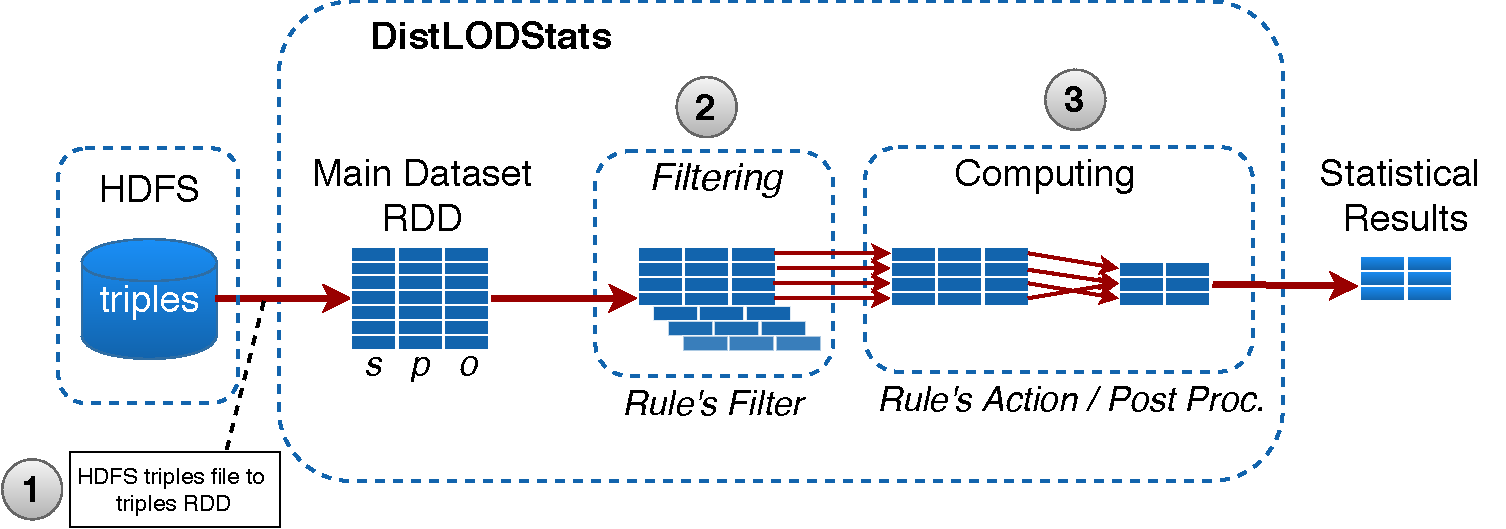
\includegraphics[width=1.0\textwidth]{images/4_distlodstats/distlodstats-system.pdf}
\caption{\textbf{Overview of DistLODStats's abstract architecture}. It is composed of three steps: First, it reads RDF data from HDFS and converts them into RDD of triples. Second, this latter undergoes a Filtering operation applying the Rule's Filter and producing a new filtered RDD. Third, the filtered RDD will serve as an input to the next step: Computing where the rule's action and/or post-processing are effectively applied. As a result, a statistical representation is generated.}
\label{fig:DistLODStatsSystem}
\end{figure*}
Furthermore, we provide a Docker image of the system\furl{https://github.com/SANSA-Stack/Spark-RDF-Statistics} available under \textit{Apache License 2.0}, integrated within the BDE platform\furl{https://github.com/big-data-europe} - an open-source Big Data Processing Platform allowing users to install numerous big data processing tools and frameworks and create working data flow applications.

We implemented DistLODStats using Spark-2.2.0, Scala 2.11.11 and Java 8. 
DistLODStats has meanwhile been integrated into SANSA~\cite{lehmann-2017-sansa-iswc,iermilov-2017-sansa-iswc-demo}, an open source\furl{https://github.com/SANSA-Stack} \emph{data flow processing engine} for performing distributed computation over large-scale \gls{RDF} datasets. 
It provides data distribution, communication, and fault tolerance for manipulating large \gls{RDF} graphs and applying machine learning algorithms on the data at scale. 
Via this integration, DistLODStats can also leverage the developer and user community as well as infrastructure behind the SANSA project. 
This also ensures the sustainability of DistLODStats given that SANSA is backed by several grants until at least 2021.


\subsection{Evaluation}
\label{sec:evaluation}
The aim of our evaluation is to see how well our approach can perform against non-distributed approaches as well as analyzing the scalability of the distributed approach. 
In particular, we addressed the following questions:   
\begin{itemize}
    \item ($Q_1$): How does the runtime of the algorithm change when more nodes in the cluster are added?
    \item ($Q_2$): How does the algorithm scale to larger datasets?
    \item ($Q_3$): How does the algorithm scale to a larger number of datasets?
\end{itemize}

In the following, we present our experimental setup including the datasets used. Thereafter, we give an overview of our results, which we subsequently discuss in the final part of this section.

\subsubsection{Experimental Setup}
We used one synthetic and two real-world datasets for our experiments:
\begin{enumerate}
 
 \item We chose the geospatial dataset LinkedGeoData~\cite{SLHA11} which offers a spatial \gls{RDF} knowledge base derived from OpenStreetMap.
 
 \item As a cross-domain dataset, we selected \emph{DBpedia}~\cite{dbpedia-swj} (v 3.9). DBpedia is a knowledge base with a large ontology.
 
 \item As a synthetic dataset, we chose to use the Berlin \gls{SPARQL} Benchmark (BSBM)~\cite{Bizer2009TheBS}.
 It is based on an e-commerce use case which is built around a set of products that are offered by different vendors.
 The benchmark provides a data generator, which can be used to create sets of connected triples of any particular size.
 
\end{enumerate}

Properties of these datasets are given in Table~\ref{tab:dataset_info}.

\begin{table*}
\centering
\begin{tabularx}{\textwidth}{Xcccccccc}	
\toprule
\multirow{2}{*}{$\longrightarrow$} & \multicolumn{1}{c}{} & \multicolumn{3}{c|}{DBpedia} & \multicolumn{3}{c}{BSBM} \\
\cline{3-9}  \rule{0pt}{10pt}
& LinkedGeoData & \scriptsize{en} & \scriptsize{de} & \scriptsize{fr}  & \scriptsize{2GB} &\scriptsize{20GB} &\scriptsize{200GB}\\
\midrule
\scriptsize{\#nr. of triples}& \scriptsize{1,292,933,812} & \scriptsize{812,545,486} & \scriptsize{336,714,883} & \scriptsize{340,849,556} & \scriptsize{8,289,484} & \scriptsize{81,980,472} & \scriptsize{817,774,057} & \\
\scriptsize{size (GB)} & \scriptsize{191.17} & \scriptsize{114.4} & \scriptsize{48.6} & \scriptsize{49.77} & \scriptsize{2} &\scriptsize{20} &\scriptsize{200} & \\
\bottomrule
\end{tabularx}
{\caption{\textbf{Dataset summary information (nt format)}.
Lists dataset characteristics used on the evaluation of the DistLODStats.
The size (in GB) and the number of triples are given.}
\label{tab:dataset_info}}
\end{table*}

For the evaluation, all data is stored on the same \gls{HDFS} cluster using Hadoop 2.8.0.
All experiments were carried out on a 6 nodes cluster (1 master, 5 workers): Intel(R) Xeon(R) CPU E5-2620 v4 @ 2.10GHz (32 Cores), 128 GB RAM, 12 TB SATA RAID-5.
The experiments on a local mode are all performed on a single instance of the cluster.
The machines were connected via a Gigabit network.
All experiments were executed three times and the average value is reported.

\subsubsection{Results}
% https://docs.google.com/spreadsheets/d/1sPdebCLTX2NK2JTvRS2TdFIPiibHWRfXT4XmBHPi0i4/edit
We evaluate our approach using the above datasets to compare it against the original LODStats.
We carried out two sets of experiments.
First, we evaluate the execution time of our distributed approach against the original approach.
Second, we evaluate the horizontal scalability via increasing nodes (machines) in the cluster. 
Results of the experiments are presented in Table~\ref{tbl:statistics}, Figure~\ref{fig:Speedup}, \ref{fig:Sizeup} and \ref{fig:Scalability}.

\defn{Distributed Processing on Large-Scale Datasets}
\label{subsubsection:large_scale_datasets}
To address $Q_1$, we started our experiments by evaluating the \textit{speedup} gained by adopting a distributed implementation of LODStats criteria using our approach, and compare it against the original centralized version.
We run the experiments on four datasets
($DBpedia_{en}$, $DBpedia_{de}$, $DBpedia_{fr}$, and $LinkedGeoData$) in a local environment on a single instance with two configurations:  (1) files of the dataset are considered separately, and (2) one big file--all files concatenated.

\begin{table*}
\centering
\begin{tabularx}{\textwidth}{Xcccccc}	
\toprule
\multicolumn{1}{l}{}& \multicolumn{5}{c}{\scriptsize{Runtime (h)} (\scriptsize{mean/std})} \\
\cline{2-6}
\rule{0pt}{8pt}
\multirow{2}{*}{$\longrightarrow$} & \multicolumn{2}{c|}{\scriptsize{\textbf{LODStats}}} & \multicolumn{3}{c}{\scriptsize{\textbf{DistLODStats}}} \\
\cline{2-6}  \rule{0pt}{10pt}
& \scriptsize{a) files} & \scriptsize{b) bigfile}  & \scriptsize{c) local} & \scriptsize{d) cluster} & \scriptsize{e) speedup ratio} \\
\midrule
\scriptsize{LinkedGeoData}& \textcolor{blue}{\scriptsize{n/a}} & \textcolor{blue}{\scriptsize{n/a}} & \scriptsize{36.65/0.13} & \win \scriptsize{4.37/0.15} & \scriptsize{7.4x}\\ \scriptsize{M$_{DBpedia}^{en}$} & \win \scriptsize{24.63/0.57} & \textcolor{red}{\scriptsize{fail}} & \scriptsize{25.34/0.11} & \win \scriptsize{2.97/0.08} & \scriptsize{7.6x} \\
\scriptsize{M$_{DBpedia}^{de}$} & \textcolor{blue}{\scriptsize{n/a}} & \textcolor{blue}{\scriptsize{n/a}} & \scriptsize{10.34/0.06} & \win \scriptsize{1.2/0.0} & \scriptsize{7.3x}\\
\scriptsize{M$_{DBpedia}^{fr}$} & \textcolor{blue}{\scriptsize{n/a}} & \textcolor{blue}{\scriptsize{n/a}} & \scriptsize{10.49/0.09} & \win \scriptsize{1.27/0.04} & \scriptsize{7.3x}\\
\bottomrule
\end{tabularx}
{\caption{\textbf{Distributed Processing on Large-Scale Datasets}.
Reports the performance analysis of the \textit{speedup} gained by DistLODStats as compared with the original centralized version.
The experiments were run on four datasets ($DBpedia_{en}$, $DBpedia_{de}$, $DBpedia_{fr}$, and $LinkedGeoData$) in a local environment on a single instance with two configurations:  (1) files of the dataset are considered separately, and (2) one big file--all files concatenated.
}
\label{tbl:statistics}}
\end{table*}

Table~\ref{tbl:statistics} shows the performance of two algorithms applied to the four datasets.
The column LODStats$^{a)}$ reports on the performance of LODStats on files separately (considering each file as a sequence of execution), the next columns LODStats$^{b)}$ reports on the performance of LODStats using a single big file by concatenating each file, and the last columns reports on the performance of DistLODStats on the same case as previously i.e. the performance for one big dataset in local mode $c)$ and cluster mode $d)$.
We observe that the execution in DistLODStats$^{c), d)}$ finishes with all the datasets (see Figure~\ref{fig:Speedup}).
However, for LODStats$^{a), b)}$ the execution often fails at different stages of the execution.
In particular, \emph{n/a} indicates parser exceptions and \emph{fail} out of memory exceptions.
The only case where the execution finishes and actually slightly outperforms DistLODStats$^{c)}$ on a single node is executing LODStats on the dataset ${DBpedia}^{en}$ split into files (25.34h for DistLODStats$^{c)}$ vs 24.63h in LODStats$^{a)}$). 
This is because the DistLODStats$^{c)}$ considers the input dataset as a big file instead of evaluation it on each file separately. 
LODStats streams the criteria one by one, so having a large dataset streamed that way would lead to very high processing times.
However, with small data as input, the processing can finish in short amount of time, but the results can be very inaccurate.

\begin{figure}
  \includegraphics[width=1.0\columnwidth]{images/4_distlodstats/distlodstats-speedup-performance.pdf}
    \caption{\textbf{Speedup performance evaluation of DistLODStats}. Reports speedup performance analysis for large-scale RDF Datasets for DistLODStats on local mode and cluster mode, respectively. All results illustrate consistent improvement for each dataset when running on a cluster. The geometric mean of the speedup is 7.4x.}
    \label{fig:Speedup}
\end{figure}

Figure~\ref{fig:Speedup} shows the speedup performance evaluation for large-scale \gls{RDF} Datasets for DistLODStats on local mode and cluster mode, respectively.
All results illustrate consistent improvement for each dataset when running on a cluster. 
The maximum speedup is 7.6x and the geometric mean of the speedup is 7.4x.

For example, on ${DBpedia}_{en}$, the time on cluster mode is about 2.97 hours which is 7.6 times faster than evaluating DistLODStats on local mode (about 25.34 hours). 
The reason why the time spent on local mode extremely decreases is that the size of the working directory of worker processes is too large and Spark uses threads for distributing the tasks.

\defn{Scalability}
\textit{Sizeup scalability} 
To measure the performance of \textit{size-up} i.e.~scalability of our approach, we run experiments on three different sizes.
This analysis keeps the number of nodes in a cluster constant, we fix the number of workers (nodes) to 5 and grow the size of datasets to measure whether a given algorithm can deal with larger datasets.
Since real-world datasets are considered to be unique in the size and also on other aspects e.g.~number of unique terms, we chose the BSBM benchmark tool to generate artificial datasets of different sizes.
We started by generating a dataset of 2GB.
Then we iteratively increased the size of datasets by one order of magnitude.

On each dataset, we ran the distributed algorithm and the runtime is reported on Figure~\ref{fig:Sizeup}.
The $x$-axis is a generated BSBM dataset per each order of 10x magnitude.

\begin{figure}
 \includegraphics[width=1.0\columnwidth]{images/4_distlodstats/distlodstats-sizeup-performance.pdf}
\caption{\textbf{Sizeup performance evaluation of DistLODStats}.
The analysis keeps the number of nodes in a cluster constant (5 worker nodes) and grows the size of datasets (BSBM) to measure whether our approach can deal with larger datasets.
We see that the execution time cost grows linearly and is near-constant when the size of the dataset increases.
It stays near-constant as long as the data fits in memory which demonstrates one of the advantages of utilizing an in-memory approach in performing the statistics computation.
}
\label{fig:Sizeup}
\end{figure}

By comparing the runtime (see Figure~\ref{fig:Sizeup}), we note that the execution time cost grows linearly and is near-constant when the size of the dataset increases.
As expected, it stays near-constant as long as the data fits in memory.
This demonstrates one of the advantages of utilizing an in-memory approach in performing the statistics computation.
The overall time spent in data read/write and network communication found in disk-based approaches is no present in distributed in-memory computing. 
The performance only starts to degrade when substantial amounts of data need to be written to disk due to memory overflows. 
The results show the scalability of our algorithm in the context of sizeup, which answers question $Q_2$.

\noindent
\textit{Node scalability} In order to measure node scalability, we use variations of the number of workers on our cluster.
The number of workers varies from 1, 2, 3 and 4 to 5.

\begin{figure}
\includegraphics[width=1.0\columnwidth]{images/4_distlodstats/distlodstats-node-scalability.pdf}
\caption{\textbf{Scalability performance evaluation on DistLODStats}.
The analysis keeps the size of the dataset constant ($BSBM_{50GB}$) and varies the number of workers on the cluster.
The number of workers varies from 1, 2, 3, and 4 to 5.
We can see that as the number of workers increases, the execution time cost is super-linear on $BSBM_{50GB}$ dataset.}
\label{fig:Scalability}
\end{figure}

Let $T_N$ be the time required to complete the task on $N$ workers. The speedup $S$ is the ratio
$ S = \frac{T_L}{T_N},$
where $T_L$ is the execution time of the algorithm on local mode.
Efficiency measures the processing power being used (i.e~speedup per worker). 
It is defined as the time to run the algorithm on $N$ workers compared to the time to run algorithm on local mode:
$ E = \frac{S}{N} =\frac{T_{L}}{N T_{N}}.$

Figure~\ref{fig:Scalability} shows the speedup for $BSBM_{50GB}$.
We can see that as the number of workers increases, the execution time cost is super-linear.

As depicted in Figure~\ref{fig:Effectiveness}, the speedup performance trend is consistent as the number of workers increases.

\begin{figure}
\includegraphics[width=1.0\columnwidth]{images/4_distlodstats/distlodstats-effectiveness.pdf}
\caption{\textbf{Speedup Ratio and Efficiency of DistLODStats}.
The speedup performance trend is consistent as the number of workers increases.
Efficiency increased only up to the 4th worker for $BSBM_{50GB}$ dataset.
The results imply that DistLODStats can achieve near-linear or even superlinear scalability in performance.}
\label{fig:Effectiveness}
\end{figure}

In contrast, as the number of workers was increased from 1 to 5, efficiency increased only up to the 4th worker for $BSBM_{50GB}$ dataset.
This implies that the tasks generated from the given dataset were covered with almost 4 nodes.
The results imply that DistLODStats can achieve near-linear or even superlinear scalability in performance, which answers question $Q_3$.

\defn{Breakdown by Criterion}\hspace*{\fill} \\
Now we analyze the overall runtime of criteria execution.
Figure~\ref{fig:Breakdown} reports on the runtime of each criterion on both $BSBM_{20GB}$ and $BSBM_{200GB}$ datasets.

\begin{figure*}
\centering
\includegraphics[width=1\columnwidth]{images/4_distlodstats/distlodstats-overall-breakdown.pdf}
\caption{\textbf{Overall Breakdown by Criterion Analysis (log scale)}.
The execution time is longer when there is data movement in the cluster compared to when data is processed without movement.
There are some criteria that are quite efficient to compute even with data movement e.g. 22, 23. 
This is because data is largely filtered before the movement.
}
\label{fig:Breakdown}
\end{figure*}

\textbf{Discussion.}
DistLODStats consists of 32 predefined criteria most of which have a runtime complexity of $O(n)$ where $n$ is the number of input triples. The breakdown for BSBM with two instances is shown in Figure~\ref{fig:Breakdown}.
The results obtained confirm to a large extent the pre-analysis made in Figure~\ref{subsection:complexAnalys}.
The execution is longer when there is data movement in the cluster compared to when data is processed without movement e.g.~Criterion \ref{cr:2}, \ref{cr:3} and \ref{cr:4}.
There are some criteria that are quite efficient to compute even with data movement e.g.~\ref{cr:22}, \ref{cr:23}. This is because data is largely filtered before the movement. 
Criterion~\ref{cr:2} and \ref{cr:28} are the most expensive ones in terms of time of execution.
This is most probably because of the sorting and maximum algorithm used by Spark.
Criteria~\ref{cr:20} and \ref{cr:21} are particularly expensive because of the extra overhead caused by extracting the data type and language for each particular object of type Literal.
Criteria like \ref{cr:14} and \ref{cr:15} do not require movement of data, but yet are inefficient in execution. This is because the data is not filtered previously.
The last three criteria do include data movement but are among the most efficient ones.
This is because the low number of namespaces the chosen datasets have.

Overall, the evaluation study conducted demonstrates that parallel and distributed computation of the different statistical values is scalable, i.e.~the execution finishes in a reasonable time relative to the high volume of datasets.


\section{STATisfy: A REST Interface for DistLODStats}
\label{sec:distlodstats-statisfy}
The increasing adoption of the Linked Data format, \gls{RDF}, over the last two decades has brought new opportunities.
It has also raised new challenges though, especially when it comes to managing and processing large amounts of \gls{RDF} data.
In particular, assessing the internal structure of a data set is important, since it enables users to understand the data better.
One prominent way of assessment is computing statistics about the instances and schema of a data set.
However, computing statistics of large \gls{RDF} data is computationally expensive.
To overcome this challenging situation, we previously built DistLODStats, a framework for parallel calculation of 32 statistical criteria over large \gls{RDF} datasets, based on Apache Spark.
Running DistLODStats is, thus, done via submitting jobs to a Spark cluster.
Often times, this process is done manually, either by connecting to the cluster machine or via a dedicated resource manager. 

SANSA and DistLODStats use Apache Spark\furl{http://spark.apache.org/} as an underlying engine, which is a popular framework for processing large datasets in-memory.
Spark provides two possibilities of running and interacting with applications: 
\begin{itemize}
    \item \textit{Interactive} - via a \gls{CLI} called \textit{Spark Shell}, or via Spark \textit{Notebooks} (e.g. SANSA-Notebooks~\cite{iermilov-2017-sansa-iswc-demo}),
    \item \textit{Batch} - which includes a bash script called \textit{spark-submit} used to submit a Spark application to the cluster without interaction during run time.
\end{itemize}

Spark application is usually launched by logging first into a cluster, either in the premises or remotely in the cloud. This process presents several difficulties:
\begin{itemize}
    \item It requires a sophisticated user access control management, which may become hard to maintain with multiple users.
    \item It raises the chances of exhausting the cluster or even causing its failure.
    \item It exposes cluster and its configurations to all the users with access.
\end{itemize}

In order to elevate those, we have investigated Apache Livy~\furl{https://livy.incubator.apache.org/} -- a novel open-source REST interface for interacting remotely with Apache Spark. It supports executing snippets of code or programs in a Spark context that runs locally, in a Spark cluster or in Apache Hadoop YARN.

\subsection{System Design Overview}
Traditionally, when running a Spark job, submitting it to a Spark cluster is done via a \textit{spark-shell} or \textit{spark-submit}.
Usually, this process is done manually either entering the cluster gateway machines or via a dedicated resource manager (e.g. SLURM, OpenStack). 

\begin{figure*}
\centering
\includegraphics[width=1.0\columnwidth]{images/4_distlodstats/distlodstats-statisfy.pdf}
\caption{\textbf{STATisfy overview architecture}.
Main services of STATisfy: \textit{Client} -- will create a remote Spark cluster for initialization, and submit jobs through REST \gls{API}s.
\textit{Livy REST Server} -- it will then discover this job and sent through \gls{RCP} to SparkSession, where the code will be initialized and executed using DistLODStats.
}
\label{fig:STATisfy}
%source:https://docs.google.com/presentation/d/1bV83Rik_xwzmYPigCwHWV9OMQC5Wtl3gSF4UoaNilIQ
\end{figure*}

For users with little experience in cluster management and the Hadoop infrastructure, it can be challenging to run Spark.
As an alternative, we introduce \textbf{STATisfy}\furl{https://github.com/GezimSejdiu/STATisfy}: REST Interface for DistLODStats. 

Instead of computing \gls{RDF} statistics directly on the cluster, the interaction is done via REST APIs (as it is depicted in the Figure~\ref{fig:STATisfy}).

The client-side will create a remote Spark cluster for initialization, and submit jobs through REST APIs. 
Livy REST Server will then discover this job and send it through \gls{RCP} to SparkSession, where the code will be initialized and executed.
In the meantime, the client will be waiting for the result of this job coming from the same direction.

Running the STATisfy is similar to using DistLODStats via \textit{spark-submit}.
The difference is that this shell is not running locally, instead, it runs in a cluster and transfers the data back and forth through the network.

For demonstrating the usage of the tool, we have deployed it on the comprehensive statistics catalog LODStats\furl{http://lodstats.aksw.org/} which crawls \gls{RDF} data from metadata portals such as CKAN dataset metadata registry. 
By doing this, it obtains a comprehensive picture of the current state of the Web of Data.
As we use DistLODStats as an underlying engine for computing \gls{RDF} statistics afterward, the limitation was that the user has to interact with the cluster manually and initiate the job for computing such statistics.
By using STATisfy REST interface, LODStats will interact with the cluster from anywhere which provides the capabilities necessary to do this without compromising on ease of use or security.

As it is shown in Figure~\ref{fig:STATisfy}, the user starts a session via REST \gls{API} using Livy for submitting a job to the Spark cluster.
With the POST request, the user could submit a request to DistLODStats using the Livy server. 
Using Livy, STATisfy will then help to launch this request in the cluster.
As a result, the output will be curled by their end in the format of the VoID description.


\section{Summary}
\label{sec:distlodstats-summary}
For obtaining an overview over the Web of Data as well as evaluating the quality of individual datasets, it is important to gather statistical information describing characteristics of the internal structure of datasets.
However, this process is both data-intensive and computing-intensive and it is a challenge to develop fast and efficient algorithms that can handle large scale \gls{RDF} datasets.

In this chapter, we presented DistLODStats, a novel software component for distributed in-memory computation of \gls{RDF} Datasets statistics implemented using the Spark framework.
DistLODStats is maintained and has an active community due to its integration in SANSA. 
Our definition of statistical criteria provides a framework reducing the implementation effort required for adding further statistical criteria. 
We showed that our approach improves upon a previous centralized approach we compare against.
Since Spark \gls{RDD}s are designed to scale horizontally, cluster sizes can be adapted to dataset sizes accordingly. 

DistLODStats is a prominent solution, however, it requires setup and managing of the cluster configuration and job submission.
To make the process easier, we have introduced STATisfy, a tool for interacting with DistLODStats via a REST Interface.
This way DistLODStats can be provided as-a-service, where users only send (HTTP) requests to the remote cluster and obtain the wished results, without having any knowledge about system access or cluster management.
STATisfy is used for the LODStats project and inclusion in the new DBpedia\furl{https://wiki.dbpedia.org/} community release processes is ongoing.
%==============================================================================
\chapter{Quality Assessment of RDF Datasets at Scale}
\label{chapter:dist_quality_assessment}
%==============================================================================
Large amounts of data are being published openly to Linked Data by different data providers. 
A multitude of applications such as semantic search, query answering, and machine reading~\cite{rw2014} depend on these large-scale\furl{http://lodstats.aksw.org/} \gls{RDF} datasets.  
The quality of underlying \gls{RDF} data plays a fundamental role in large-scale data consuming applications. 
Measuring the quality of linked data spans a number of dimensions including but not limited to: accessibility, interlinking, performance, syntactic validity or completeness~\cite{zaveri2015quality}.
Each of these dimensions can be expressed through one or more quality metrics. 
Considering that each quality metric tries to capture a particular aspect of the underlying data, numerous metrics are usually provided against the given data that may or may not be processed simultaneously.

On the other hand, the limited number of existing techniques of quality assessment for \gls{RDF} datasets are not adequate to assess data quality at large-scale and these approaches mostly fail to capture the increasing volume of big data. 
To date, a limited number of solutions have been conceived to offer a quality assessment of \gls{RDF} datasets \cite{Debattista0AC18,farber2018,beek2018,debattista2016luzzu}.
But, these methods can either be used on a small portion of large datasets \cite{farber2018} or narrow down to specific problems e.g., syntactic accuracy of literal values~\cite{beek2018}, or accessibility of resources~\cite{Mihindukulasooriya2016LDSA}.
In general, these existing efforts show severe deficiencies in terms of performance when data grows beyond the capabilities of a single machine.
This limits the applicability of existing solutions to medium-sized datasets only, in turn, paralyzing the role of applications in embracing the increasing volumes of the available datasets.

To deal with big data, tools like Apache Spark\furl{https://spark.apache.org/} have recently gained a lot of interest. 
Apache Spark provides scalability, resilience, and efficiency for dealing with large-scale data. 
Spark uses the concepts of \gls{RDD}~\cite{zaharia2012resilient} and performs operations like transformations and actions on this data in order to effectively deal with large-scale data. 

To handle large-scale \gls{RDF} data, it is important to develop flexible and extensible methods that can assess the quality of data at scale. 
At the same time, due to the broadness and variety of quality assessment domain and resulting metrics, there is a strong need to provide a generic pattern to characterize the quality assessment of \gls{RDF} data in terms of scalability and applicability to big data.

In this chapter, we borrow the concepts of data \textit{transformation} and \textit{action} from Spark and present a pattern for designing quality assessment metrics over large \gls{RDF} datasets, which is inspired by design patterns.
In software engineering, design patterns are general and reusable solutions to common problems. 
Akin to design pattern, where each pattern acts like a blueprint that can be customized to solve a particular design problem, 
the introduced concept of Quality Assessment Pattern ($\mathcal{QAP}$) represents a generalized blueprint of scalable quality assessment metrics. 
In this way, the quality metrics designed following $\mathcal{QAP}$ can exhibit the ability to achieve scalability to large-scale data and work in a distributed manner.
In addition, we also provide an open source implementation and assessment of these quality metrics in Apache Spark following the proposed $\mathcal{QAP}$.

In this chapter we address the following research question:

\begin{tcolorbox}
\textbf{RQ2}: Can quality of large-scale \gls{RDF} Datasets be assessed efficiently in a distributed manner?
\end{tcolorbox}

Contributions of this chapter are summarize as follows:
\begin{itemize}
    \item We present a Quality Assessment Pattern $\mathcal{QAP}$ to characterize scalable quality metrics.
    \item We provide DistQualityAssessment -- a distributed (open source) implementation of quality metrics using Apache Spark.
    \item We perform an analysis of the complexity of the metric evaluation in the cluster.
    \item We evaluate our approach and demonstrate empirically its superiority over a previous centralized approach.
    \item We integrated the approach into the SANSA framework.
    SANSA is actively maintained and uses the community ecosystem (mailing list, issues trackers, continuous integration, website, etc.).
\end{itemize}


This chapter is based on the following publication (\cite{sejdiu-2019-sansa-dist-quality-assessment-iswc}):
\begin{itemize}
     \item \textbf{Gezim Sejdiu}; Anisa Rula; Jens Lehmann; and Hajira Jabeen, “\href{http://jens-lehmann.org/files/2019/iswc_dist_quality_assessment.pdf}{A Scalable Framework for Quality Assessment of RDF Datasets},” in Proceedings of 18th International Semantic Web Conference (ISWC), 2019.
\end{itemize}

The remainder of this chapter is organized as follows:
Our approach for the computation of \gls{RDF} dataset quality metrics is detailed in Section~\ref{sec:distqualityassessment-approach} and evaluated in Section~\ref{sec:distqualityassessment-evaluation}.
Finally, we summarize our work in  Section~\ref{sec:distqualityassesment-summary}.

\section{A Scalable Framework for Quality Assessment of RDF Datasets}
\label{sec:distqualityassessment-approach}
In this section, we first introduce the basic notions used in our approach, the formal definition of the proposed quality assessment pattern and then describe the workflow. 

\subsection{Quality Assessment Pattern}
Data quality is commonly conceived as a multi-dimensional construct~\cite{BatiniS16} with a popular notion of 'fitness for use' and can be measured along many dimensions $\mathcal{D}$ such as accuracy ($d_{accu} \in \mathcal{D}$), completeness ($d_{comp} \in \mathcal{D}$) and timeliness ($d_{tmls} \in \mathcal{D}$). 
The assessment of a quality dimensions $d$ is based on quality metrics $\mathcal{QM} = \{m_1,m_2,~\dots~m_k\}$ where $m_i$ is a heuristic that is designed to fit a specific assessment dimension. 
The following definitions form the basis of $\mathcal{QAP}$.

\begin{definition}[Filter]
Let $\mathcal{F} = \{f_1,f_2,~\dots~f_l\}$ be a set of filters where each filter $f_i$ sets a criteria for extracting predicates, objects, subjects, or their combination.
A filter $f_i$ takes a set of \gls{RDF} triples as input and returns a subgraph that satisfies the filtering criteria.
\end{definition}

\begin{definition}[Rule]
Let $\mathcal{R} = \{r_1,r_2,~\dots~r_j\}$ be a set of rules where each rule $r_i$ sets a conditional criteria. A rule takes a subgraph as input and returns a new subgraph that satisfies the conditions posed by the rule $r_i$.
\end{definition}

\begin{definition}[Transformation]
\label{def:tr}
A \textit{transformation} $\tau:\mathcal{G} \rightarrow \mathcal{G'}$ is an operation that applies rules defined by $\mathcal{R}$ on the \gls{RDF} graph $\mathcal{G}$ and returns an \gls{RDF} subgraph $\mathcal{G'}$. 
A transformation $\tau$ can be a union $\cup$ or intersection $\cap$ of other transformations. 
\end{definition}

\begin{definition}[Action]
\label{def:ac}
An \textit{action} $ \alpha: \mathcal{G}\rightarrow \mathbb{R}$ is an operation that triggers the transformation of rules on the filtered \gls{RDF} graph $\mathcal{G'}$ and generates a numerical value. 
Action $\alpha$ is the count of elements obtained after performing a $\tau$ operation.
\end{definition}

\begin{definition}[Quality Assessment Pattern $\mathcal{QAP}$]
\label{def:QAP}
The Quality Assessment Pattern $\mathcal{QAP}$ is a reusable template to implement and design scalable quality metrics. %$\mathcal{QM}$ 
The $\mathcal{QAP}$ is composed of \textit{transformations} and \textit{actions}. 
The output of a $\mathcal{QAP}$ is the outcome of an action returning a numeric value against the particular metric.
\end{definition}

$\mathcal{QAP}$ is inspired by Apache Spark operations and designed to fit different data quality metrics (for more details see Table~\ref{Table:QM}). 

\begin{table}[t]
\centering
\begin{tabular}{>{\scriptsize}l>{\scriptsize}l>{\scriptsize}l}
    \verb|Quality Metric| &  \verb|:=| &  \verb|Action|   \textbar   \verb|(Action| $\mathcal{OP} $  \verb|Action)|\\
    $\mathcal{OP} $   &  \verb|:=| & $\mathcal{*}$ \textbar  $\mathcal{-}$ \textbar / \textbar $\mathcal{+}$ \\
  %$\mathcal{OP} $   & $\mathcal{* \textbar  - \textbar / \textbar + }$ \\
 \verb|Action| &  \verb|:=| & \verb|Count(Transformation)| \\
 \verb|Transformation|  &  \verb|:=| &  \verb|Rule(Filter)| \textbar  \verb|(Transformation BOP Transformation)| \\
 \verb|Filter| &  \verb|:=| &  \verb|getPredicates|  $\sim ?p$ \textbar  \verb|getSubjects|  $ \sim ?s$ \textbar  \verb|getObjects| $\sim ?o$ \textbar  \verb|getDistinct(Filter)|\\
 && \textbar  \verb|Filter or Filter|  \textbar  \verb|Filter && Filter)|\\
 
 
 \verb|Rule| &  \verb|:=| &  \verb|isURI(Filter)| \textbar  \verb|isIRI(Filter)| \textbar  \verb|isInternal(Filter)| \textbar  \verb|isLiteral(Filter)|\\
&& \textbar  \verb|!isBroken(Filter)|  \textbar  \verb|hasPredicateP| \textbar   \verb|hasLicenceAssociated(Filter)| \\
&& \textbar  \verb|hasLicenceIndications(Filter)|  \textbar 
 \verb|isExternal(Filter)| \textbar  \verb|hasType((Filter)|\\
&&  \textbar \verb|isLabeled(Filter)| \\
 \verb|BOP| &  \verb|:=| & $\cap$ | $\cup$ \\
 \bottomrule
\end{tabular}
\caption{\textbf{Quality Assessment Pattern}.
A reusable template for quality metric implementation composed of transformations and actions.}
\label{Table:QM}
\end{table}

Each data \textit{quality metric} can be defined following the $\mathcal{QAP}$. 
Any given data quality metric $m_i$ that is represented through the $\mathcal{QAP}$ using transformation $\tau$ and action $\alpha$ operations can be easily transformed into Spark code to achieve scalability.

Table~\ref{tab:MetricRules} demonstrates a few selected quality metrics defined against proposed $\mathcal{QAP}$. 

\begin{table*}
    \centering
    \begin{tabular}{>{\scriptsize}l>{\scriptsize}l|>{\scriptsize}l>{\scriptsize}l|>{\scriptsize}l}
      \textbf{} & 
      \textbf{Metric} & 
      \multicolumn{2}{l|}{\textbf{\scriptsize Transformation $\tau$}} & 
      \textbf{Action $\alpha$} \\ 
        \hline  
        \newMetricNr[L1]\label{qm:L1} 
        & Detection of a & 
      \verb|r = hasLicenceAssociated(?p)| & & $\alpha$ \verb| = count(r)|  \\
       & 
     Machine Readable License & 
      & & $\alpha$ \verb| > 0 ? 1 : 0| \\
     \hline  
    \newMetricNr[L2]\label{qm:L2} 
    & Detection of a Human & 
    \verb|r = isURI(?s)| $ \cap $  \verb|hasLicenceIndications(?p)| $ \cap $  \verb|| & & $\alpha$ \verb| = count(r)| \\
    & Readable License & 
    \quad \quad \verb|isLiteral(?o)| $ \cap $  \verb|isLicenseStatement(?o)| & & $\alpha$ \verb| > 0 ? 1 : 0| \\
    \hline  
    \newMetricNr[I2]\label{qm:I2} 
    & Linkage Degree of Linked & 
      \verb|r_1 = isIRI(?s)| $\cap$  \verb|internal(?s)| $ \cap $ & 
      & $\alpha$\verb|_1 = count(r_3)| \\
    & External Data Providers  & 
     \quad \quad \quad \verb|isIRI(?o)| $ \cap $  \verb|external(?o)| & 
      & $\alpha$\verb|_2 = count(triples)|\\
    & & 
      \verb|r_2 = isIRI(?s)| $ \cap $  \verb|external(?s)| $ \cap $ & & $\alpha$\verb| = a_1/a_2| \\
    &  & 
     \quad \quad \quad \verb|isIRI(?o) | $ \cap $  \verb|internal(?o) | & 
      &  \\
    &  & 
      \verb|r_3 = r_1| $\cup$ \verb|r_2| & 
      & \\
    \hline  
    \newMetricNr[U1]\label{qm:U1} 
    & Detection of a Human & 
    \verb|r_1 = isURI(?s)| $ \cap $ \verb|isInternal(?s)| $ \cap $ & & $\alpha$\verb|_1 = count(r_1) +| \\
    & Readable Labels & 
     \quad \quad \quad  \verb|isLabeled(?p)| & & \quad \quad \quad \verb|count(r_2) +| \\
     &  & 
    \verb|r_2 = isInternal(?p)| $\cap$ \verb|isLabeled(?p)| & & \quad \quad \quad \verb|count(r_3)| \\
    & & 
    \verb|r_3 = isURI(?o)| $ \cap $ \verb|isInternal(?o)| $\cap$ & & $\alpha$\verb|_2 = count(triples)| \\
    & & \quad \quad \quad \verb|isLabeled(?p)| & & $\alpha$\verb|_1/| $\alpha$\verb|_2| \\
    \hline  
    \newMetricNr[RC1]\label{qm:RC1} 
    & Short URIs & 
      \verb|r_1 = isURI(?s)| $\cup$ \verb|isURI(?p)| $\cup$ \verb|isURI(?o)| & & $\alpha$\verb|_1 =count(r_2)| \\
    & & \verb|r_2 = resTooLong(?s, ?p, ?o)| & & $\alpha$\verb|_1/count(triples)| \\
    \hline  
    \newMetricNr[SV3]\label{qm:SV3} 
    & Identification of Literals & 
      \verb|r = isLiteral(?o)| $\cap$  \verb|getDatatype(?o)| $\cap$  &  & $\alpha$\verb| = count(r)| \\
    & with Malformed Datatypes & 
    \quad \quad \verb|isLexicalFormCompatibleWithDatatype(?o)| &  &   \\
     \hline  
    \newMetricNr[CN2]\label{qm:CN2} 
    & Extensional Conciseness & 
      \verb|r = isURI(?s)| $\cap$  \verb|isURI(?o)| &  & %\verb|M[reduce(?s,?p)]++| \\
      $\alpha$\verb|_1 = count(r)| \\
      &  & &  & $\alpha$\verb|_2 = count(triples)| \\
      &  & &  &\verb|(|$\alpha$\verb|_2-| $\alpha$\verb|_1)/| $\alpha$\verb|_2| \\
      \end{tabular}
\caption{\textbf{Definition of selected metrics following $\mathcal{QAP}$}.
List of few selected quality metrics defined against proposed QAP.}
\label{tab:MetricRules}
\end{table*}

As shown in Table~\ref{tab:MetricRules}, each quality metric can contain multiple rules, filters or actions. 
It is worth mentioning that action $\verb|count(triples)|$ returns the total number of triples in the given data. 
This can also be seen that the action can be an arithmetic combination of multiple actions i.e. ratio, sum, etc. 
We illustrate our proposed approach on some metrics selected from~\cite{debattista2016luzzu,zaveri2015quality}. 
Given that the aim of this paper is to show the applicability of the proposed approach and comparison with existing methods, we have only selected those which are already provided out-of-box in Luzzu.


\subsection{System Overview}
In this section, we give an overall description of the data model and the architecture of DistQualityAssessment.
We model and store \gls{RDF} graphs $\mathcal{G}$ based on the basic building block of the Spark framework, \gls{RDD}s. 
\gls{RDD}s are in-memory collections of records that can be operated in parallel on a large distributed cluster.
\gls{RDD}s provide an interface based on \emph{coarse-grained} transformations (e.g \emph{map}, \emph{filter} and \emph{reduce}): operations applied on an entire \gls{RDD}. 
A \emph{map} function transforms each value from an input \gls{RDD} into another value while applying $\tau$ rules.
A \emph{filter} transforms an input \gls{RDD} to an output \gls{RDD}, which contains only the elements that satisfy a given condition.
\emph{Reduce} aggregates the \gls{RDD} elements using a specific function from $\tau$.

The computation of the set of quality metrics $\mathcal{QM}$ is performed using Spark as depicted in Figure~\ref{fig:DistQualityAssessmentSystem}.
Our approach consists of four steps: 

\begin{figure*}
\centering
\includegraphics[width=1.0\columnwidth]{images/5_distqualityassessment/distqualityassessment-architecture.pdf}
\caption{\textbf{Overview of distributed quality assessment's abstract architecture}.
Main components of DistQualityAssessment: 1) Definitions -- defining quality metrics parameters, 2) Retrieving the RDF data, 3) Parsing and mapping RDF data into the main dataset (RDD of triples), and 4) Quality metric evaluation.}
\label{fig:DistQualityAssessmentSystem}
\end{figure*}
% source: https://docs.google.com/presentation/d/1JP_urfFpIzPKH4z1TXKSN3d00TmzbQ2YxGL7nQ7-IgI

\defn{Defining quality metrics parameters (Step 1)} The metric definitions are kept in a dedicated file that contains most of the configurations needed for the system to evaluate quality metrics and gather result sets.

\defn{Retrieving the \gls{RDF} data (Step 2)} \gls{RDF} data first needs to be loaded into a large-scale storage that Spark can efficiently read from.
We use \gls{HDFS}.
\gls{HDFS} is able to fit and stores any type of data in its Hadoop-native format and parallelizes them across a cluster while replicating them for fault tolerance.
In such a distributed environment, Spark automatically adopts different data locality strategies to perform computations as close to the needed data as possible in \gls{HDFS} and thus avoids data transfer overhead.
 
\defn{Parsing and mapping \gls{RDF} into the main dataset (Step 3)} We first create a distributed dataset called \emph{main dataset} that represent the \gls{HDFS} file as a collection of triples.
In Spark, this dataset is parsed and loaded into an \gls{RDD} of triples having the format 
\emph{Triple$<$(s,p,o)$>$}.

\defn{Quality metric evaluation (Step 4)} Considering the particular quality metric, Spark generates an execution plan, which is composed of one or more $\tau$ transformations and $\alpha$ actions. 
The numerical output of the final action is the quality of the input \gls{RDF} corresponding to the given metric.

\subsection{Implementation}
\label{subsection:distqualityassessment-implementation}
We have used the Scala\furl{https://www.scala-lang.org/} programming language \gls{API} in Apache Spark to provide the distributed implementation of the proposed approach. 

\begin{algorithm}
\caption{Spark-based parallel quality assessment algorithm.}
\label{alg:DistQualityAssessment}
\SetKwInOut{Input}{input}\SetKwInOut{Output}{output}
\Input{$RDF$: an RDF dataset,
	   $param$: quality metrics parameters.
      }
\Output{$dqv$ description or $metric$ numerical value}
    $\textit{triples} = spark.\textbf{rdf}(lang)(input)$ \label{line:qa-rdf2rdd} \\
    $\textit{triples}.persist()$ \label{line:qa-cache}\\
    $dqv \leftarrow \emptyset$ \\
    \ForEach{$m \in param.getListOfMetrics$}{
        $triples \leftarrow triples.Tranform~\{~t =>$ \label{line:qa-filter} \\
        $\quad \quad \textit{rule} \leftarrow m.Rule$ \\
        $\quad \quad t.apply(rule)~\}~$ \\
        $metric \leftarrow triples.apply(m.Action)$  \label{line:qa-action}\\
        \If{m.hasDQVdescription}{
            $dqvify \leftarrow metric.dqvify()$ \label{line:dqvify}
        }
        $dqv.add(dqvify)$
    }
\Return{$(dqv, metric)$} \label{line:qa-result}
\end{algorithm}

The DistQualityAssessment (see Algorithm~\ref{alg:DistQualityAssessment}) constructs the \emph{main dataset} (Line \ref{line:qa-rdf2rdd}) while reading \gls{RDF} data (e.g. NTriples file or any other \gls{RDF} serialization format) and converts it into an \gls{RDD} of triples.
This latter undergoes the transformation operation of applying the filtering through rules in $R$ and producing a new \emph{filtered} \gls{RDD} ($\mathcal{G'}$) (Line \ref{line:qa-filter}).
At the end, $\mathcal{G'}$ will serve as an input to the next step which applies a set of $\alpha$ actions (Line \ref{line:qa-action}).
The output of this step is the metric output represented as a numerical value (Line \ref{line:qa-action}). 
The result set of different quality metrics (Line \ref{line:qa-result}) can be further visualized and monitored using SANSA-Notebooks~\cite{iermilov-2017-sansa-iswc-demo}.\\
The user can also choose to extract the output in a machine-readable format (Line \ref{line:dqvify}). 
We have used the data quality vocabulary (DQV)~\cite{Isaac:16:dqv} to represent the quality metrics. 

Furthermore, we also provide a Docker image of the system integrated within the BDE platform\furl{https://github.com/big-data-europe} - an open-source Big Data processing platform allowing users to install numerous big data processing tools and frameworks and create working data flow applications.

The work done here (available under \textit{Apache License 2.0}) has been integrated into SANSA~\cite{lehmann-2017-sansa-iswc}, an open source\furl{https://github.com/SANSA-Stack} \emph{data flow processing engine} for scalable processing of large-scale \gls{RDF} datasets. 
SANSA uses Spark offering fault-tolerant, highly available and scalable approaches to process massive sized datasets efficiently. 
SANSA provides the facilities for semantic data representation, querying, inference, and analytics at scale.
Being part of this integration, DistQualityAssessment can take advantage of having the same user community as well as infrastructure build via the SANSA project.
Doing so, it can also ensure the sustainability of the tool given that SANSA is supported by several grants until at least 2021.

\paragraph{\textbf{Complexity Analysis}}
We deem that the overall time complexity of the distributed quality assessment evaluation is $O(n)$.
The performance of metrics computation depends on data shuffling (while filtering using rules in $R$) and data scanning. 
Our approach performs a direct mapping of any quality metric designed using $\mathcal{QAP}$ into a sequence of Spark-compliant Scala-commands, as a consequence, most of the operators used are a series of transformations like $map$, $filter$ and $reduce$.
The complexity of $map$ and $filter$ is considered to be linear with respect to the number of triples associated with it. 
The complexity of a metric then depends on the $\alpha$ operation that returns the count of the filtered output.
This later step works on the distributed \gls{RDD} between $p$ nodes which implies that the complexity of each node then becomes $O(n/p)$, where $n$ is a number of input triples.
Let be $O(\tau)$ a complexity of $\tau$, then the complexity of the metric will be $O(n/p*O(\tau))$.
This indicates that the runtime increases linearly when the size of an \gls{RDD} increases and decreases linearly when more nodes $p$ are added to the cluster.


\section{Evaluation}
\label{sec:distqualityassessment-evaluation}
The main aim of DistQualityAssessment is to serve massive large-scale real-life \gls{RDF} datasets. 
We are interested in addressing the following additional questions.

\begin{itemize}
    \item \textbf{Flexibility}: How fast our approach processes different types of metrics?
    \item \textbf{Scalability}: How large are the \gls{RDF} datasets that DistQualityAssessment can scale to? 
    What is the system speedup w.r.t the number of nodes in a cluster mode?
    \item \textbf{Efficiency}: How well our approach performs compared with other state-of-the-art systems on real-world datasets?
\end{itemize}
In the following, we present our experimental setup including the datasets used. 
Thereafter, we give an overview of our results.

\subsection{Experimental Setup}
We chose two real-world and one synthetic datasets for our experiments:
 \begin{enumerate}
 \item \emph{DBpedia}~\cite{dbpedia-swj} (v 3.9) -- a cross domain dataset.
 DBpedia is a knowledge base with a large ontology.
 We build a set of 3 pipelines of increasing complexity: (i) $M_{DBpedia}^{en}$ ($\approx$ 813M triples); (ii) $M_{DBpedia}^{de}$ ($\approx$ 337M triples); (iii) $M_{DBpedia}^{fr}$ ($\approx$ 341M triples). 
DBpedia has been chosen because of its popularity in the Semantic Web community.
\item \emph{LinkedGeoData}~\cite{SLHA11} -- a spatial \gls{RDF} knowledge base derived from OpenStreetMap.
\item \emph{Berlin \gls{SPARQL} Benchmark (BSBM})~\cite{Bizer2009TheBS}  -- a synthetic dataset based on an e-commerce use case containing a set of products that are offered by different vendors and reviews posted by consumers about products.
The benchmark provides a data generator, which can be used to create sets of connected triples of any particular size.
 \end{enumerate}
Properties of the considered datasets are given in Table~\ref{tab:qa-dataset_info}.

\begin{table*}
\centering
\begin{tabularx}{\textwidth}{Xcccccccc}	
\toprule
\multirow{2}{*}{$\longrightarrow$} & \multicolumn{1}{c}{} & \multicolumn{3}{c|}{DBpedia} & \multicolumn{4}{c}{BSBM} \\
\cline{3-9}  \rule{0pt}{10pt}
& LinkedGeoData & \scriptsize{en} & \scriptsize{de} & \scriptsize{fr}  & \scriptsize{2GB} &\scriptsize{20GB} &\scriptsize{200GB} &\\
\midrule
\scriptsize{\#nr. of triples}& \scriptsize{1,292,933,812} & \scriptsize{812,545,486} & \scriptsize{336,714,883} & \scriptsize{340,849,556} & \scriptsize{8,289,484} & \scriptsize{81,980,472} & \scriptsize{817,774,057} &  \\
\scriptsize{size (GB)} & \scriptsize{191.17} & \scriptsize{114.4} & \scriptsize{48.6} & \scriptsize{49.77} & \scriptsize{2} &\scriptsize{20} &\scriptsize{200} &\\
\bottomrule
\end{tabularx}
{\caption{\textbf{Dataset summary information (nt format)}.
Lists dataset information used on the evaluation of the DistQualityAssessment.
The size (in GB) and the number of triples are given.}
\label{tab:qa-dataset_info}}
\end{table*}

We implemented DistQualityAssessment using Spark-2.4.0, Scala 2.11.11 and Java 8, and all the data were stored on the \gls{HDFS} cluster using Hadoop 2.8.0.
The experiments in local mode are all performed on a single instance of the cluster.
Specifically, we compare our approach with Luzzu~\cite{debattista2016luzzu} v4.0.0, a state-of-the-art quality assessment system\furl{https://github.com/Luzzu/Framework}.
All distributed experiments were carried out on a small cluster of 7 nodes (1 master, 6 workers): Intel(R) Xeon(R) CPU E5-2620 v4 @ 2.10GHz (32 Cores), 128 GB RAM, 12 TB SATA RAID-5.
The machines were connected via a Gigabit network.
All experiments have been executed three times and the average value is reported in the results.

\subsection{Results}
%source: https://docs.google.com/spreadsheets/d/1RrwtYbJFhd2g8U4V5OTrWT1sd6ujtZopvWyAIIlJqnQ
We evaluate the proposed approach using the above datasets to compare it against Luzzu~\cite{debattista2016luzzu}.
We carry out two sets of experiments.
First, we evaluate the runtime of our distributed approach in contrast to Luzzu.
Second, we evaluate the horizontal scalability via increasing nodes in the cluster.
Results of the experiments are presented in Table~\ref{tbl:distqualityassessment-performance-evaluation}, Figure~\ref{fig:distqualityassessment-sizeup-scalability} and
\ref{fig:distqualityassessment-node-scalability}.
Based on the metric definition, some metrics make use of external access (e.g. Dereferenceability of Forward Links) which leads to a significant increase in Spark processing due to network latency. 
For the sake of the evaluation, we have suspended such metrics.
As of that, we choose seven metrics (see Table~\ref{tab:MetricRules} for more details) where the level of difficulty varies from simple to complex according to the combination of transformation/action operations involved.

\subsubsection{Performance evaluation on large-scale RDF datasets}
\label{subsubsection:distqualityassessment-large_scale_datasets}
We started our experiments by evaluating the \textit{speedup} gained by adopting a distributed implementation of quality assessment metrics using our approach, and compare it against Luzzu.
We run the experiments on five datasets
($DBpedia_{en}$, $DBpedia_{de}$, $DBpedia_{fr}$, $LinkedGeoData$ and $BSBM_{200GB}$).
Local mode represents a single instance of the cluster without any tuning of Spark configuration and the cluster mode includes further tuning.
Luzzu was run in a local environment on a single machine with two strategies: (1) streaming the data for each metric separately, and (2) one stream/load -- all metrics evaluated just once. 

\begin{table*}
\centering
\begin{tabularx}{\textwidth}{Xcccccc}	
\toprule
\multicolumn{1}{l}{}& \multicolumn{5}{c}{\scriptsize{Runtime (m)} (\scriptsize{mean/std})} \\
\cline{2-6}
\rule{0pt}{8pt}
\multirow{2}{*}{$\longrightarrow$} & \multicolumn{2}{c|}{\scriptsize{\textbf{Luzzu}}} & \multicolumn{3}{c}{\scriptsize{\textbf{DistQualityAssessment}}} \\
\cline{2-6}  \rule{0pt}{10pt}
& \scriptsize{a) single} & \scriptsize{b) joint}  & \scriptsize{c) local} & \scriptsize{d) cluster} & \scriptsize{e) speedup ratio w.r.t} \\
& & & & & \scriptsize{Luzzu \textbar DistQualityAssessment$^{c)}$} \\
\midrule
\multirow{5}{*}{\rotatebox{90}{\textbf{Large-scale}}}
$LinkedGeoData$ & \textcolor{red}{\scriptsize{Fail}} & \textcolor{red}{\scriptsize{Fail}} & \scriptsize{446.9/63.34} & \win \scriptsize{7.79/0.54} & \win \scriptsize{n/a\textbar56.4x}\\
\hspace{0.2cm} $DBpedia_{en}$ & \textcolor{red}{\scriptsize{Fail}} & \textcolor{red}{\scriptsize{Fail}} & \scriptsize{274.31/38.17} & \win \scriptsize{1.99/0.04} & \win \scriptsize{n/a\textbar136.8x} \\
\hspace{0.2cm} $DBpedia_{de}$ & \textcolor{red}{\scriptsize{Fail}} & \textcolor{red}{\scriptsize{Fail}} & \scriptsize{161.4/24.18} & \win \scriptsize{0.46/0.04} & \win \scriptsize{n/a\textbar349.9x}\\
\hspace{0.2cm} $DBpedia_{fr}$ & \textcolor{red}{\scriptsize{Fail}} & \textcolor{red}{\scriptsize{Fail}} & \scriptsize{195.3/26.16} & \win \scriptsize{0.38/0.04} & \win \scriptsize{n/a\textbar512.9x}\\
\hspace{0.2cm} $BSBM_{200GB}$ & \textcolor{red}{\scriptsize{Fail}} & \textcolor{red}{\scriptsize{Fail}} & \scriptsize{454.46/78.04} & \win \scriptsize{7.27/0.64} & \win \scriptsize{n/a\textbar61.5x}\\
\midrule
\multirow{10}{*}{\rotatebox{90}{\textbf{Small to medium}}}
$BSBM_{0.01GB}$ & \scriptsize{2.64/0.02} & \scriptsize{2.65/0.01} & \win \scriptsize{0.04/0.0} & \scriptsize{0.42/0.04} & \win \scriptsize{65x\textbar (-0.9x)}\\
\hspace{0.2cm} $BSBM_{0.02GB}$ & \scriptsize{5.9/0.16} & \scriptsize{5.66/0.02} & \win \scriptsize{0.04/0.0} & \scriptsize{0.43/0.03} & \win \scriptsize{146.5x\textbar (-0.9x)}\\
\hspace{0.2cm} $BSBM_{0.05GB}$ & \scriptsize{16.38/0.44} & \scriptsize{15.39/0.21} & \win \scriptsize{0.05/0.0} & \scriptsize{0.46/0.02} & \win \scriptsize{326.6x\textbar (-0.9x)}\\
\hspace{0.2cm} $BSBM_{0.1GB}$ & \scriptsize{40.59/0.56} & \scriptsize{37.94/0.28} & \win \scriptsize{0.06/0.0} & \scriptsize{0.44/0.05} & \win \scriptsize{675.5x\textbar (-0.9x)}\\
\hspace{0.2cm} $BSBM_{0.2GB}$ & \scriptsize{101.8/0.72} & \scriptsize{101.78/0.64} & \win \scriptsize{0.07/0.0} & \scriptsize{0.4/0.03} & \win \scriptsize{1453.3\textbar (-0.8x)}\\
\hspace{0.2cm} $BSBM_{0.5GB}$ & \scriptsize{459.19/18.72} & \scriptsize{468.64/21.7} & \win \scriptsize{0.15/0.01} & \scriptsize{0.48/0.03} & \win \scriptsize{3060.3x\textbar (-0.7x)}\\
\hspace{0.2cm} $BSBM_{1GB}$ & \scriptsize{1454.16/10.55} & \scriptsize{1532.95/51.6} & \win \scriptsize{0.4/0.02} & \scriptsize{0.56/0.02} & \win \scriptsize{3634.4x\textbar (-0.3x)}\\
\hspace{0.2cm} $BSBM_{2GB}$ & \textcolor{blue}{\scriptsize{Timeout}} & \textcolor{blue}{\scriptsize{Timeout}} & \scriptsize{3.19/0.16} & \win \scriptsize{0.62/0.04} & \win \scriptsize{n/a\textbar 4.1x}\\
\hspace{0.2cm} $BSBM_{10GB}$ & \textcolor{blue}{\scriptsize{Timeout}} & \textcolor{blue}{\scriptsize{Timeout}} & \scriptsize{29.44/0.14} & \win \scriptsize{0.52/0.01} & \win \scriptsize{n/a\textbar 55.6x}\\
\hspace{0.2cm} $BSBM_{20GB}$ & \textcolor{red}{\scriptsize{Fail}} & \textcolor{red}{\scriptsize{Fail}} & \scriptsize{34.32/9.22} & \win \scriptsize{0.75/0.29} & \win \scriptsize{n/a\textbar 44.8x}\\
\bottomrule
\end{tabularx}
{\caption{\textbf{Performance evaluation on large-scale RDF datasets}.
A \textit{speedup} analysis gained by DistQualityAssessment as compared with Luzzu.
The experiments were run on five datasets
($DBpedia_{en}$, $DBpedia_{de}$, $DBpedia_{fr}$, $LinkedGeoData$ and $BSBM_{200GB}$).
Luzzu was run in a local environment on a single machine with two strategies: (1) streaming the data for each metric separately, and (2) one stream/load -- all metrics evaluated just once.
}
\label{tbl:distqualityassessment-performance-evaluation}}
\end{table*}

Table~\ref{tbl:distqualityassessment-performance-evaluation} shows the performance of two approaches applied to five datasets.
In Table~\ref{tbl:distqualityassessment-performance-evaluation} we indicate "Timeout" whenever the process did not complete within a certain amount of time\f{We set the timeout delay to 24 hours of the quality assessment evaluation stage.} and "Fail" when the system crashed before this timeout delay.
%Fail message : Exception in thread "main" org.apache.jena.ext.com.google.common.util.concurrent.ExecutionError: java.lang.OutOfMemoryError: GC overhead limit exceeded
Column Luzzu$^{a)}$ represents the performance of Luzzu on bulk load -- considering each metric as a sequence of the execution, on the other hand, the column Luzzu$^{b)}$ reports on the performance of Luzzu using a joint load by evaluating each metric using one load.
The last columns reports on the performance of DistQualityAssessment run on a local mode $c)$, cluster mode $d)$ and speedup ratio of our approach compared to Luzzu$^{b)}$ ($d)/b)-1$) and itself evaluated on local mode ($d)/c)-1$) is reported on the column $e)$.
We observe that the execution of our approach finishes with all the datasets whereas this is not the case with Luzzu which either timeout or fail at some point.

Unfortunately, Luzzu was not capable of evaluating the metrics over large-scale \gls{RDF} datasets from Table~\ref{tbl:distqualityassessment-performance-evaluation} (part one). 
For that reason, we run yet another set of experiments on very small datasets that Luzzu was able to handle. 
The second part of the Table~\ref{tbl:distqualityassessment-performance-evaluation} shows a performance evaluation of our approach compared with Luzzu on very small \gls{RDF} datasets.
In some cases (e.g. \ref{qm:RC1}, \ref{qm:SV3}) for a very small dataset, Luzzu performs better than our approach with a small margin of runtime in the local mode.
It is due to the fact that in the streaming model when Luzzu$^{a)}$ finds the first statement which fulfills the condition (e.g.finding the shortest \gls{URI}s), it stops the evaluation and returns the results.
On the contrary, our approach evaluates the metrics over the whole dataset exploiting the fault-tolerance and resilient features build-in Spark.
In other cases, Luzzu suffers from significant slowdowns, which are several orders of magnitude slower.
Therefore, its average runtime over all metrics is worst as compared to our approach. 
It is important to note that our approach to these very small datasets degrades while running on the cluster mode.
This is because of the network overhead while shuffling the data, but it outperforms Luzzu$^{a),b)}$ when considering ''average runtime'' over all the metrics (even for very small datasets).

Findings shown in Table~\ref{tbl:distqualityassessment-performance-evaluation} depicts that our approach starts outperforming when the size of the dataset grows (e.g. $BSBM_{2GB}$).
The runtime in the cluster mode stays constant when the size of the data fits into the main memory of the cluster.
On other hand, Luzzu is not able to evaluate the metrics when the size of data starts increasing, the time taken lasts beyond the delay we set for small datasets. 
Because of the large differences, we have used a logarithmic scale to better visualize these results.

\subsubsection{Scalability performance analysis}
\label{subsubsection:distqualityassessment-scalability_performance}
In this experiment, we evaluate the efficiency of our approach.
Figure~\ref{fig:distqualityassessment-sizeup-scalability} and \ref{fig:distqualityassessment-node-scalability} illustrates the results of the comparative efficiency analysis.

\begin{figure*}
\centering
 \includegraphics[width=1.0\columnwidth]{images/5_distqualityassessment/distqualityassessment-sizeup-scalability.pdf}
    \caption{\textbf{Sizeup performance evaluation of DistQualityAssessment}.
    The analysis fixes the number of nodes to 6 and grows the size of datasets to measure whether DistQualityAssessment can deal with larger datasets.
    We see that the execution time increases linearly and is near-constant when the size of the dataset increases. 
    As expected, it stays near-constant as long as the data fits in memory.}
    \label{fig:distqualityassessment-sizeup-scalability}
\end{figure*}

\textit{Data scalability} 
To measure the performance of \textit{size-up} scalability of our approach, we run experiments on five different sizes.

We fix the number of nodes to 6 and grow the size of datasets to measure whether DistQualityAssessment can deal with larger datasets.
For this set of experiments, we consider BSBM benchmark tool to generate synthetic datasets of different sizes since the real-world dataset is considered to be unique in their size and attributes.

We start by generating a dataset of 2GB.
Then, we iteratively increase the size of datasets.
On each dataset, we run our approach and the runtime is reported on Figure~\ref{fig:distqualityassessment-sizeup-scalability}.
The $x$-axis shows the size of the BSBM dataset with an increasing order of 10x magnitude.

By comparing the runtime (see Figure~\ref{fig:distqualityassessment-sizeup-scalability}), we note that the execution time increases linearly and is near-constant when the size of the dataset increases.
As expected, it stays near-constant as long as the data fits in memory.
This demonstrates one of the advantages of utilizing the in-memory approach for performing quality assessment computation.
The overall time spent in data read/write and network communication found in disk-based approaches is saved.
However, when the data overflows the memory, and it is spilled to disk, the performance degrades.
These results show the scalability of our algorithm in the context of size-up.

\textit{Node scalability} In order to measure node scalability, we vary the number of workers on our cluster.
The number of workers has varied from 1, 2, 3, 4 and 5 to 6.

\begin{figure*}
\centering
  \includegraphics[width=1.0\columnwidth]{images/5_distqualityassessment/distqualityassessment-node-scalability.pdf}
    \caption{\textbf{Node scalability performance evaluation of DistQualityAssessment}.
    The analysis keeps the size of the dataset constant ($BSBM_{200GB}$) and varies the number of workers on the cluster.
    The number of workers varies from 1, 2, 3, 4 and 5 to 6.
    We can see that as the number of workers increases, the execution time cost-decrease is almost linear. 
    It decreases about 14 times (from 433.31 minutes down to 28.8 minutes) as cluster nodes increase from one to six worker nodes. The results shown here imply that our approach can achieve near-linear scalability in performance in the context of speedup.}
    \label{fig:distqualityassessment-node-scalability}
\end{figure*}

Figure~\ref{fig:distqualityassessment-node-scalability} shows the speedup for $BSBM_{200GB}$ with the various number of worker nodes.
We can see that as the number of workers increases, the execution time cost-decrease is almost linear.
The execution time decreases about 14 times (from 433.31 minutes down to 28.8 minutes) as cluster nodes increase from one to six worker nodes.
The results shown here imply that our approach can achieve near-linear scalability in performance in the context of speedup.

Furthermore, we conduct the effectiveness evaluation of our approach.
Speedup $S$ is an important metric to evaluate a parallel algorithm.
It is defined as a ratio $S=T_s/T_n$, where $T_s$ represents the execution time of the algorithm run on a single node and $T_n$ represents the execution time required for the same algorithm on $n$ nodes with the same configuration and resources.
Efficiency is defined as a ratio $E = S/n =T_s/n T_n$ which measures the processing power being used, in our case the speedup per node.

\begin{figure*}
\includegraphics[width=1.0\columnwidth]{images/5_distqualityassessment/distqualityassessment-effectiveness.pdf}
\caption{\textbf{Effectiveness of DistQualityAssessment}.
The speedup performance trend shows that it achieves almost linear speedup and even superlinear in some cases.
The speedup grows faster than the number of worker nodes due to the computation task for the metric being computationally intensive, and the data does not fit in the cache when executed on a single node but fits into several machines when the workload is divided amongst the cluster for parallel evaluation.
}
\label{fig:distqualityassessment-effectiveness}
\end{figure*}

The speedup and efficiency curves of DistQualityAssessment are shown in Figure~\ref{fig:distqualityassessment-effectiveness}.
The trend shows that it achieves almost linear speedup and even superlinear in some cases.
The upper curve in the Figure~\ref{fig:distqualityassessment-effectiveness} indicates superlinear speedup. 
The speedup grows faster than the number of worker nodes.
This is due to the computation task for the metric being computationally intensive, and the data does not fit in the cache when executed on a single node. 
But it fits into the caches of several machines when the workload is divided amongst the cluster for parallel evaluation.
While using Spark, the superlinear speedup is an outcome of the improved complexity and runtime, in addition to efficient memory management behavior of the parallel execution environment.

\subsubsection{Correctness of metrics}
In order to test the correctness of implemented metrics, we assess the numerical values for metrics like \ref{qm:L1}, \ref{qm:L2}, and \ref{qm:RC1} on very small datasets and the results are found correct w.r.t Luzzu. 
For metrics like \ref{qm:I2} and \ref{qm:CN2}, Luzzu uses approximate values for faster performance, and that is not the same as getting the exact number as in the case of our implementation.

\subsubsection{Overall analysis by metrics}
We analyze the overall run-time of the metric evaluation.
Figure~\ref{fig:distqualityassessment-overall-analysis} reports on the run-time of each metric considered in this paper (see Table~\ref{tab:MetricRules}) on both $BSBM_{20GB}$ and $BSBM_{200GB}$ datasets.

\begin{figure*}
\includegraphics[width=1.0\columnwidth]{images/5_distqualityassessment/distqualityassessment-overall-analysis.pdf}
\caption{\textbf{Overall analysis of by metric in the cluster mode (log scale)}.
It shows that the execution is sometimes a little longer when there is a shuffling involved in the cluster compared to when data is processed without movement e.g. Metric L2 and L1. 
Metric SV3 and CN2 are the most expensive ones in terms of runtime. This is due to the extra overhead caused by extracting the literals for objects and checking the lexical form of its datatype.
}
\label{fig:distqualityassessment-overall-analysis}
\end{figure*}

DistQualityAssessment implements predefined quality assessment metrics from \cite{zaveri2015quality}. 
We have implemented these metrics in a distributed manner such that most of them have a run-time complexity of $O(n)$ where $n$ is the number of input triples.
The overall performance of analysis for the BSBM dataset with two instances is shown in Figure~\ref{fig:distqualityassessment-overall-analysis}.
The results obtained show that the execution is sometimes a little longer when there is a shuffling involved in the cluster compared to when data is processed without movement e.g.~Metric \ref{qm:L2} and \ref{qm:L1}.
Metric~\ref{qm:SV3} and \ref{qm:CN2} are the most expensive ones in terms of runtime.
This is due to the extra overhead caused by extracting the literals for objects, and checking the lexical form of its datatype. 

Overall, the evaluation study carried out in this paper demonstrates that distributed computation of  different quality measures is scalable and the execution ends in reasonable time given the large volume of data.


\section{Summary}
\label{sec:distqualityassesment-summary}
The data quality assessment becomes challenging with the increasing sizes of data.
Many existing tools mostly contain a customized data quality functionality to detect and analyze data quality issues within their own domain. 
However, this process is both data-intensive and computing-intensive and it is a challenge to develop fast and efficient algorithms that can handle large scale \gls{RDF} datasets.

In this thesis, we have introduced DistQualityAssessment, a novel approach for distributed in-memory evaluation of \gls{RDF} quality assessment metrics implemented on top of the Spark framework.
The presented approach offers generic features to solve common data quality checks.
As a consequence, this can enable further applications to build trusted data utilities. 

We have demonstrated empirically that our approach improves upon the previous centralized approach that we have compared against.
The benefit of using Spark is that its core concepts (\gls{RDD}s) are designed to scale horizontally. 
Users can adapt the cluster sizes corresponding to the data sizes, by dropping when it is not needed and adding more when there is a need for it.
%==============================================================================
\chapter{Scalable RDF Querying}
\label{chapter:scalable_rdf_querying}
%==============================================================================
In recent years, our information society has reached the stage where it produces billions of data records, amounting to multiple quintillions of bytes\furl{https://www.domo.com/learn/data-never-sleeps-5}, on a daily basis.
Extraction, cleansing, enrichment and refinement of information are key to fuel value-adding processes, such as analytics as a premise for decision making.
Devising appropriate (ideally uniform) representations and facilitating efficient querying of data, metadata, and provenance arising from such phases constantly poses challenges, especially when data volumes are vast.
The most prominent and promising effort is the \gls{W3C} consortium with encouraging \gls{RDF} as a common data representation and vocabularies (e.g. \gls{RDFS}, \gls{OWL}) as a way to include meta-information about the data.
These data and meta-data can be further processed and analyzed using the de-facto query language for \gls{RDF} data, \gls{SPARQL}.
\gls{SPARQL} serves as a standard query language for manipulating and retrieving \gls{RDF} data.

Querying \gls{RDF} data becomes challenging when the size of the data increases. 
This has motivated a considerable amount of work on designing distributed \gls{RDF} systems able to efficiently evaluate \gls{SPARQL} queries (\cite{Schatzle:2016:SRQ:2977797.2977806,sparqlgx-iswc-2016}).
Being able to query a large amount of data in an efficient and faster way is one of the key requirements for every \gls{SPARQL} engine.

To address these challenges, in this thesis, we propose a scalable \gls{RDF} querying engine based on two different partitioning strategies.
First, Sparklify -- SPARQL-to-SQL rewriter based on the vertical partitioning~\cite{VPAbadi2007} implemented on top of Apache Spark.
As a second approach, we investigated and developed the so-called Semantic-based query system. 
Both approaches are a scalable and efficient evaluation of \gls{SPARQL} queries over distributed \gls{RDF} datasets. 
The main component of the both systems are the data partitioning and query evaluation over this data representation.

In this chapter we address the following research question:
\begin{tcolorbox}
\textbf{RQ3}: Can distributed \gls{RDF} datasets be queried efficiently and effectively?
\end{tcolorbox}

Contributions of this chapter are summarized as follows:

\begin{itemize}
 \item We present a novel approach for vertical partitioning including \gls{RDF} terms using the distributed computing framework, Apache Spark.
 \item We developed a scalable query system using Sparqlify -- a SPARQL-to-SQL rewriter on top of Apache Spark (under the \textit{Apache Licence 2.0}).
 \item We evaluate Sparklify with state-of-the-art engines and demonstrate it empirically.
 \item A scalable approach for semantic-based partitioning using the distributed computing framework, Apache Spark.
 \item A scalable semantic-based query engine (\textit{SANSA.Semantic}) on top of Apache Spark.
 \item Comparison of the semantic-based system with state-of-the-art engines and demonstrate the performance empirically.
 \item We integrated the proposed approaches into the SANSA~\cite{lehmann-2017-sansa-iswc}\furl{http://sansa-stack.net/} larger framework.
 Sparklify serves as a default query engine in SANSA.
 SANSA is an active project and maintained, including issue tracker, mailing list, changelogs, website, etc.
\end{itemize}


This chapter is based on the following publications (\cite{sejdiu-2019-sansa-semantic-based-semantics,2019-sansa-sparklify-iswc, sansa-sparklify-ISWC-demo}):
\begin{itemize}
    \item \textbf{Gezim Sejdiu}; Damien Graux; Imran Khan; Ioanna Lytra; Hajira Jabeen; and Jens Lehmann, “\href{https://gezimsejdiu.github.io/publications/semantic_based_query_paper_SEMANTICS2019.pdf}{Towards A Scalable Semantic-based Distributed Approach for SPARQL query evaluation},” 15th International Conference on Semantic Systems (SEMANTiCS), Research \& Innovation , 2019.
     
    \item Claus Stadler; \textbf{Gezim Sejdiu}; Damien Graux; and Jens Lehmann, “\href{http://jens-lehmann.org/files/2019/iswc_sparklify.pdf}{Sparklify: A Scalable Software Component for Efficient evaluation of SPARQL queries over distributed RDF datasets},” in Proceedings of 18th International Semantic Web Conference (ISWC), 2019. 
    This article is a joint work with Claus Stadler, a PhD student at the University of Leipzig. 
    In this article, I devised the implementation of the conceptual architecture, helped on the implementation of the proposed approach, reviewed related work, and preparation of the experiments and analysis of the obtained results.
    
    \item Claus Stadler; \textbf{Gezim Sejdiu}; Damien Graux; and Jens Lehmann. "\href{https://gezimsejdiu.github.io/publications/sansa-sparklify-ISWC-demo.pdf}{Querying large-scale RDF datasets using the SANSA framework}".  In Proceedings of 18th International Semantic Web Conference (ISWC), Poster \& Demos, 2019.
    This demonstration article is a joint work with Claus Stadler, a PhD student at the University of Leipzig.
    In this article, I helped in describing the architecture and implementation of the running example.
\end{itemize}

The rest of the chapter is structured as follows:
Sparklify, a scalable software component for \gls{SPARQL} evaluation of large \gls{RDF} data is presented in Section~\ref{sec:sparklify-approach}.
Its data modeling, data partitioning, and query translation using a distributed framework (Apache Spark) are detailed in Subsection~\ref{sec:sparklify-architecture} and evaluated in Subsection~\ref{sec:sparklify-evaluation}.
Second part of the chapter, Section~\ref{sec:semantic-based-approach} elaborate the Semantic-based approach, including its system architecture overview as presented in Section~\ref{fig:semantic-based-architecture}.
The Semantic-based approach is evaluated in Subsection~\ref{sec:semantic-based-evaluation}.
Finally, we summarize our work in  Section~\ref{sec:scalable-rdf-querying-summary}.

\section{Sparklify: A Scalable Software for SPARQL Evaluation of Large RDF Data}
\label{sec:sparklify-approach}
In this section, we present the overall architecture of Sparklify, the SPARQL-to-SQL rewriter, and mapping to Spark Scala-compliant code.

\subsection{System Architecture Overview}
\label{sec:sparklify-architecture}
The overall system architecture is shown in Figure~\ref{fig:sparklify-architecture}.
It consists of four main components: Data Model, Mappings, Query Translator and Query Evaluator.
In the following, each component is discussed in details.

\begin{figure*}
\centering
\includegraphics[width=1.0\textwidth]{images/6_scalable_rdf_querying/sparklify-architecture.pdf}
\caption{\textbf{Sparklify Architecture Overview}.
It consists of four main components: Data modeling -- data ingestion and data partitioning (using the extensible VP), Mappings/Views -- the relational-to-RDF mapping, Query Translator -- SQL query generator from the SPARQL query, and Query Evaluator - SQL query evaluated directly into the Spark SQL engine.
}
% source : https://docs.google.com/presentation/d/16XlT4u3bFn8XdP_eoLJOAu5WPl_q_9zIjAZbllfEEic 
\label{fig:sparklify-architecture}
% source : 
\end{figure*}

\defn{Data Model}
SANSA~\cite{lehmann-2017-sansa-iswc} comes with different data structures and different partitioning strategies.
We model and store \gls{RDF} graph following the concept of \gls{RDD}s -- a basic building blocks of the Spark Framework.
\gls{RDD}s are in-memory collections of records that are capable of operating in a parallel overall larger cluster.
Sparklify makes use of the SANSA bottom layer which corresponds with the extended \gls{VP} including \gls{RDF} terms.
This partition model is the most convenient storage model for the fast processing of \gls{RDF} datasets on top of \gls{HDFS}.
\paragraph{Data Ingestion (Step 1)} \gls{RDF} data first needs to be loaded into a large-scale storage that Spark can efficiently read from.
We use \gls{HDFS}.
Spark employ different data locality scheme in order to accomplish computations nearest to the desired data in \gls{HDFS}, as a result avoiding i/o overhead. 
\paragraph{Data Partition (Step 2)}
\gls{VP} approach in SANSA is designed to support the extensible partitioning of \gls{RDF} data.
Instead of dealing with a single three-column table $(s, p, o)$, data is partitioned into multiple tables based on the used \gls{RDF} predicates, \gls{RDF} term types and literal datatypes.
The first column of these tables is always a string representing the subject.
The second column always represents the literal value as a Scala/Java datatype.
Tables for storing literals with language tags have an additional third-string column for the language tag.

\defn{Mappings/Views}
After the \gls{RDF} data has been partitioned using the extensible \gls{VP} (as it has been described on \textit{Step 2}) the relational-to-RDF mapping is performed. 
Sparqlify supports both the \gls{W3C} standard R2RML
sparqlification~\cite{sml}.

The main entities defined with SML are \textit{view definitions}.
See \textit{Step 5} in the Figure~\ref{fig:sparklify-architecture} as an example.
The actual view definition is declared by the \emph{Create View} \ldots \emph{As} in the first line.
The remainder of the view contains these parts: (1) the \emph{From} directive defines the logical table based on the partitioned table (see \textit{Step 2}).
(2) an \gls{RDF} template is defined in the \emph{Construct} block containing, \gls{URI}, blank node or literals constants (e.g. \emph{ex:worksAt}) and variables (e.g. \emph{?emp}, \emph{?institute}).
The \emph{With} block defines the variables used in the template by means of \gls{RDF} term constructor expressions whose arguments refer to columns of the logical table.

\defn{Query Translation}
This process generates a SQL query from the \gls{SPARQL} query using the bindings determined in the mapping/view construction phases.
It walks through the \gls{SPARQL} query (\textit{Step 4}) using Jena ARQ\furl{https://jena.apache.org/documentation/query/} and generates the \gls{SPARQL} \gls{AET}. 
Essentially, rewriting \gls{SPARQL} basic graph patterns and filters over views yields \gls{AET}s that are UNIONS of JOINS.
Further, these \gls{AET}s are normalized and pruned in order to remove UNION members that are known to yield empty results, such as joins based on \gls{IRI}s with disjoint sets of known namespaces, or joins between different \gls{RDF} term types (e.g. literal and \gls{IRI}).
Finally, the SQL is generated (\textit{Step 6}) using the bindings corresponding to the views (\textit{Step 5}).

\defn{Query Evaluator}
The SQL query created as described in the previous section can now be evaluated directly into the Spark SQL engine.
The result set of this SQL query is distributed data structure of Spark (e.g. DataFrame) (\textit{Step 7}) which then is mapped into a \gls{SPARQL} bindings.
The result set can further used for analysis and visualization using the SANSA-Notebooks (\textit{Step 8})~\cite{iermilov-2017-sansa-iswc-demo}.


\subsection{Evaluation}
\label{sec:sparklify-evaluation}
The goal of our evaluation is to observe the impact of the extensible \gls{VP} as well as analyzing its scalability when the size of the dataset increases.
At the same time, we also want to measure the effect of using Sparqlify optimizer for improving query performance.
Especially, we want to verify and answer the following questions:
\begin{itemize}
\addtolength{\itemindent}{1cm}
    \newitem[Q1]\label{item:Q1}: Is the runtime affected when more nodes are added in the cluster?
    \newitem[Q2]\label{item:Q2}: Does it scale to a larger dataset?
    \newitem[Q3]\label{item:Q3}: How does it scale when adding a larger number of datasets?
\end{itemize}
In the following, we present our experiment setting including the benchmarks used and server configurations. 
Afterword, we elaborate on our findings.

\subsubsection{Experimental Setup}
We used two well-known \gls{SPARQL} benchmarks for our evaluation. 
The \textit{Lehight University Benchmak (LUBM)} v3.1~\cite{Guo2005LUBMAB} and \textit{Waterloo \gls{SPARQL} Diversity Test Suite (WatDiv)} v0.6~\cite{Alu2014DiversifiedST}.
Characteristics of the considered datasets are given in Table~\ref{tab:sparklify-dataset_info}.

\textit{LUBM} comes with a \textit{Data Generator (UBA)} which generates synthetic data over the \textit{Univ-Bench} ontology in the unit of a university.
Our \textit{LUBM} datasets consist of 1000, 5000, and 10000 universities.
The number of triples varies from 138M for 1000 universities, to 1.4B triples for 10000 universities.
\textit{LUBM}'s test suite is comprised of 14 queries.

We have used \textit{WatDiv} datasets with approximate 10K to 1B triples with scale factors 10, 100 and 1000, respectively. 
\textit{WatDiv} provides a test suite with different query shapes, therefore, it allows us to compare the performance of Sparklify and the other approach we compare within a more compact way.
We have generated these queries using the \textit{WatDiv Query Generator} and report the average mean runtime in the overall results presented below.
It comes with a set of 20 predefined query templates so-called \textit{Basic Testing Use Case} which is grouped into four categories, based on the query shape : \textit{star (QS)}, \textit{linear (QL)}, \textit{snowflake (QF)}, and \textit{complex (QC)}.

\begin{table*}
\centering
\begin{tabularx}{\textwidth}{Xccccccc}	
\toprule
\multirow{2}{*}{$\longrightarrow$} & \multicolumn{3}{c|}{LUBM} & \multicolumn{4}{c}{Watdiv} \\
\cline{2-8}  \rule{0pt}{10pt}
&   \scriptsize{1K} & \scriptsize{5K} & \scriptsize{10K}  & \scriptsize{10M} &\scriptsize{100M} &\scriptsize{1B} &\\
\midrule
\scriptsize{\#nr. of triples}& \scriptsize{138,280,374} & \scriptsize{690,895,862} & \scriptsize{1,381,692,508} & \scriptsize{10,916,457} & \scriptsize{108,997,714} & \scriptsize{1,099,208,068} &  \\
\scriptsize{size (GB)}  & \scriptsize{24} & \scriptsize{116} & \scriptsize{232} & \scriptsize{1.5} &\scriptsize{15} &\scriptsize{149} &\\
\bottomrule
\end{tabularx}
{\caption{\textbf{Summary information of used datasets (nt format)}.
Lists dataset characteristics used on the evaluation.
The size (in GB) and the number of triples are given.}
\label{tab:sparklify-dataset_info}}
\end{table*}

We implemented Sparklify using Spark-2.4.0, Scala 2.11.11, Java 8, and Sparqlify 0.8.3 and all the data were stored on the \gls{HDFS} cluster using Hadoop 2.8.0.
All experiments were carried out on a commodity cluster of 7 nodes (1 master, 6 workers): Intel(R) Xeon(R) CPU E5-2620 v4 @ 2.10GHz (32 Cores), 128 GB RAM, 12 TB SATA RAID-5, connected via a Gigabit network.
The experiments have been executed three times and the average runtime has been reported into the results.

\subsubsection{Results}
We evaluate Sparklify using the above datasets and compare it with the chosen state-of-the-art distributed \gls{SPARQL} query evaluator.
Since our approach does not involve any pre-processing of the \gls{RDF} data before being able to evaluate \gls{SPARQL} queries on it, Sparklify is thereby closer to the so-called direct evaluators.
Indeed, Sparklify only needs to virtually partition the data prior.
As a consequence, we omit other distributed evaluators (such as e.g. S2RDF~\cite{Schatzle:2016:SRQ:2977797.2977806}) and compare it with SPARQGX~\cite{sparqlgx-iswc-2016} as it outperforms other approaches as noted by Graux et.al~\cite{sparqlgx-iswc-2016}.
We compare our approach with \emph{SPARQLGX}'s direct evaluator named SDE and report the loading time for partitioning and query execution time, see Table~\ref{tbl:sparklify-performance-analysis}.
We specify ``fail'' whenever the system fails to complete the task and ``n/a'' when the task could not be completed due to a failure in one of the intermediate phase.
In some cases e.g. in Table~\ref{tbl:sparklify-performance-analysis}, \textit{QC in Watdiv-1B} dataset, we define "partial fail" due to the failure of one of the queries, therefore the sum-up is not possible.

Findings of the experiments are depicted in Table~\ref{tbl:sparklify-performance-analysis}, Figure~\ref{fig:sparklify-sizeup-scalability}, \ref{fig:sparklify-node-scalability}, and  \ref{fig:sparklify-overall-analysis}.

To verify \ref{item:Q1}, we analyze the \textit{speedup} and compare it with SPARQLGX.
We run the experiments on three datasets, \emph{Watdiv-10M}, \emph{Watdiv-1B} and \emph{LUBM-10K}.

\begin{table*}[t]
\centering
\begin{tabularx}{\textwidth}{*{6}{X}}	
\toprule
\multicolumn{1}{l}{}& \multicolumn{4}{c}{\scriptsize{Runtime (s)} (\scriptsize{mean})} \\
\cline{2-5}
\rule{0pt}{8pt}
\multirow{2}{*}{$\longrightarrow$} & \multicolumn{1}{c|}{\scriptsize{\textbf{SPARQLGX-SDE}}} & \multicolumn{3}{c}{\scriptsize{\textbf{Sparklify}}} \\
\cline{2-5}  \rule{0pt}{10pt}
& \scriptsize{a) total} & \scriptsize{b) paritioning}  & \scriptsize{c) querying} & \scriptsize{d) total} \\
\midrule
\multirow{5}{*}{\rotatebox{90}{\scriptsize{\textbf{Watdiv-10M}}}}
&  & & & \\
\hspace{0.2cm} $QC$ & \win \scriptsize{103.24} & \scriptsize{134.81} & \win \scriptsize{61} & \scriptsize{195.84} \\
\hspace{0.2cm} $QF$ & \win \scriptsize{157.8} & \scriptsize{241.24} & \win \scriptsize{107.33} & \scriptsize{349.51}  \\
\hspace{0.2cm} $QL$ & \win \scriptsize{102.51} & \scriptsize{236.06} & \scriptsize{134} & \scriptsize{370.3} \\
\hspace{0.2cm} $QS$ & \win \scriptsize{131.16} & \scriptsize{237.12} & \win \scriptsize{108.56} & \scriptsize{346} \\
\midrule
\multirow{5}{*}{\rotatebox{90}{\scriptsize{\textbf{Watdiv-1B}}}}
&  & & &  \\
\hspace{0.2cm} $QC$ & \textcolor{red}{\scriptsize{partial fail} }& \win \scriptsize{778.62} & \win \scriptsize{2043.66} & \win \scriptsize{2829.56} \\
\hspace{0.2cm} $QF$ & \scriptsize{6734.68} & \win \scriptsize{1295.31} & \win \scriptsize{2576.52} & \win \scriptsize{3871.97} \\
\hspace{0.2cm} $QL$ & \scriptsize{2575.72} & \win \scriptsize{1275.22} & \win \scriptsize{610.66} & \win \scriptsize{1886.73} \\
\hspace{0.2cm} $QS$ & \scriptsize{4841.85} & \win \scriptsize{1290.72} & \win \scriptsize{1552.05} & \win \scriptsize{2845.3} \\
\midrule
\multirow{14}{*}{\rotatebox{90}{\scriptsize{\textbf{LUBM-10K}}}}
$Q1$ & \win \scriptsize{1056.83} & \scriptsize{627.72} & \scriptsize{718.11} & \scriptsize{1346.8}\\
\hspace{0.2cm} $Q2$ & \textcolor{red}{\scriptsize{fail}} & \scriptsize{595.76} & \textcolor{red}{\scriptsize{fail}} &  \scriptsize{n/a} \\
\hspace{0.2cm} $Q3$ & \win \scriptsize{1038.62} & \scriptsize{615.95} & \scriptsize{648.63} &  \scriptsize{1267.37} \\
\hspace{0.2cm} $Q4$ & \scriptsize{2761.11} & \win \scriptsize{632.93} & \win \scriptsize{1670.18} &  \win \scriptsize{2303.18} \\
\hspace{0.2cm} $Q5$ & \win \scriptsize{1026.94} & \scriptsize{641.53} & \scriptsize{564.13} &  \scriptsize{1206.67}\\
\hspace{0.2cm} $Q6$ & \win \scriptsize{537.65} & \scriptsize{695.74} & \scriptsize{267.48} &  \scriptsize{963.62}\\
\hspace{0.2cm} $Q7$ & \scriptsize{2080.67} & \win \scriptsize{630.44} & \win \scriptsize{1331.13} &  \win \scriptsize{1967.25}\\
\hspace{0.2cm} $Q8$ & \scriptsize{2636.12} & \win \scriptsize{639.93} & \win \scriptsize{1647.57} &  \win \scriptsize{2288.48} \\
\hspace{0.2cm} $Q9$ & \scriptsize{3124.52} & \win \scriptsize{583.86} & \win \scriptsize{2126.03} &  \win \scriptsize{2711.24} \\
\hspace{0.2cm} $Q10$ & \win \scriptsize{1002.56} & \scriptsize{593.68} & \scriptsize{693.73} &  \scriptsize{1287.71} \\
\hspace{0.2cm} $Q11$ & \win \scriptsize{1023.32} & \scriptsize{594.41} & \scriptsize{522.24} &  \scriptsize{1118.58}\\
\hspace{0.2cm} $Q12$ & \scriptsize{2027.59} & \win \scriptsize{576.31} & \win \scriptsize{1088.25} &  \win \scriptsize{1665.87} \\
\hspace{0.2cm} $Q13$ & \scriptsize{1007.39} & \win \scriptsize{626.57} & \win \scriptsize{6.66} &  \win \scriptsize{633.26} \\
\hspace{0.2cm} $Q14$ & \win \scriptsize{526.15} & \scriptsize{633.39} & \scriptsize{258.32} &  \scriptsize{891.89}\\
\bottomrule
\end{tabularx}
{\caption{\textbf{Performance analysis on large-scale RDF datasets}.
Comparison analysis of Sparklify as compared with \emph{SPARQLGX}'s direct evaluator named SDE.
The loading time for partitioning and query execution time is reported.
}
\label{tbl:sparklify-performance-analysis}}
\end{table*} %source : https://docs.google.com/spreadsheets/d/16CcsZcmrGF0yevu8L5mlAALGB2JZvHNkS4-6WQV0edo

Table~\ref{tbl:sparklify-performance-analysis} shows the performance analysis of two approaches run on three different datasets.
Column SPARQLGX-SDE$^{a}$ reports on the performance of SPARQLGX-SDE considering the total runtime to evaluate the given queries.
Column Sparklify$^{b}$ lists the times required for Sparklify to perform the \gls{VP} and then the query execution time is reported on the Sparklify$^{c}$.
Total runtime for Sparklify is shown in the last column, Sparklify$^{d}$.

We observe that the execution of both approaches fails for the \textit{Q2} in the \textit{LUBM-10K} dataset while evaluating the query. 
We believe that it is due to the reason that \textit{LUBM Q2} involves a triangular pattern which is often resource consuming. 
As a consequence, in both cases, Spark performs the shuffling (e.g. data scanning) while reducing the result set.
It is interesting to note that for the \textit{Watdiv-1B} dataset, SPARQLGX-SDE fails for the query \textit{C3} when data scanning is performed. 
Sparklify is capable of evaluating it successfully.
Due to the Spark SQL optimizer in conjunction with Sparqlify's approach of rewriting a SPARQL query typically into only a single SQL query -- effectively offloading all query planning to Spark -- Sparklify performs better than SPARQLGX-SDE when the size of the dataset increases (see \textit{Watdiv-1B results} in the Table~\ref{tbl:sparklify-performance-analysis}) and when there are more joins involved (see \textit{Watdiv-1B} and \textit{LUBM-10K} results in the Table~\ref{tbl:sparklify-performance-analysis}).
SPARQLGX-SDE evaluates the queries faster when the size of the datasets is smaller, but it degrades when the size of the dataset increases.
The likely reason for Sparklify's worse performance on smaller datasets is its higher partitioning overhead.
Figure~\ref{fig:sparklify-sizeup-scalability} shows that Sparklify starts outperforming when the size of the datasets grows (e.g. \textit{Watdiv-100M}).

\defn{Size-up scalability analysis}
To measure the performance of the data scalability (e.g. size-up) of both approaches, we run experiments on three different sizes of \textit{Watdiv} (see Figure~\ref{fig:sparklify-sizeup-scalability}).

\begin{figure*}
 \includegraphics[width=1.0\columnwidth]{images/6_scalable_rdf_querying/sparklify-sizeup-scalability.pdf}
    \caption{\textbf{Sizeup analysis (on Watdiv dataset)}.
    The analysis keeps the number of nodes constant i.e. 6 worker nodes and grow the size of the dataset (Watdiv) in order to measure whether the approaches chosen for evaluation can deal with larger datasets.
    As depicted, the execution time for Sparklify grows linearly as compared with SPARQLGX-SDE, and keep staying near-linear when the size of the dataset increases.}
    \label{fig:sparklify-sizeup-scalability}
\end{figure*}

We keep the number of nodes constant i.e 6 worker nodes and grow the size of the datasets to measure whether both approaches can deal with larger datasets.
We see that the execution time for Sparklify grows linearly compared with SPARQLGX-SDE, which keeps staying as near-linear when the size of the datasets increases. 
The results presented show the scalability of Sparklify in the context of the sizeup, which addresses the question \ref{item:Q2}.

\defn{Node scalability analysis}
To measure the node scalability of Sparklify, we vary the number of worker nodes.
We vary them from 1, 3 to 6 worker nodes.

\begin{figure*}
  \includegraphics[width=1.0\columnwidth]{images/6_scalable_rdf_querying/sparklify-node-scalability.pdf}
    \caption{\textbf{Node scalability (on Watdiv-100M)}.
    The analysis varies the number of worker nodes e.g. from 1, 3, to 6 worker nodes and keeps the size of the dataset constant i.e. \textit{Watdiv-100M}.
    It shows that as the number of nodes increases, the runtime cost for Sparklify decreases linearly.
    It decreases about 0.6 times (from 2547.26 seconds down to 1588.4 seconds) as worker nodes increase from one to three nodes.}
    \label{fig:sparklify-node-scalability}
\end{figure*}

Figure~\ref{fig:sparklify-node-scalability} depict the speedup performance of both approaches run on \textit{Watdiv-100M} dataset when the number of worker nodes varies.
We can see that as the number of nodes increases, the runtime cost for the Sparklify decreases linearly.
The execution time for Sparklify decreases about 0.6 times (from 2547.26 seconds down to 1588.4 seconds) as worker nodes increase from one to three nodes.
We see that the speedup stays constant when more worker nodes are added since the size of the data is not that large and the network overhead increases a little the runtime when it runs over six worker nodes.
This implies that our approach is efficient up to three worker nodes for the \textit{Watdiv-100M} (15GB) dataset.
In another hand, SPARQLGX-SDE takes longer to evaluate the queries when running on one worker node but it improves when the number of worker nodes increases.

Result presented here shows that Sparklify can achieve linear scalability in the performance, which addresses \ref{item:Q3}.

\defn{Correctness of the result set}
In order to assess the correctness of the result set, we computed the count of the result set for the given queries and compare it within both approaches.
We conclude that both approaches return exactly the same result set which implies the correctness of the results.

\defn{Overall analysis by \gls{SPARQL} queries}
Here we analyze Watdiv queries run on \textit{Watdiv-100M} dataset in a cluster mode on both approaches.

\begin{figure}
  \includegraphics[width=1.0\columnwidth]{images/6_scalable_rdf_querying/sparklify-overall-analysis.pdf}
    \caption{\textbf{Overall analysis of queries on the Watdiv-100M dataset (cluster mode)}.
    This analysis gives more insights about running Watdiv queries on \textit{Watdiv-100M} dataset in a cluster mode on both approaches, Sparklify and SPARQLGX-SDE.
    The findings show that SPARQLGX-SDE performance decreases as the number of triple patterns involved in the query increase.
    In contrast to SPARQLGX-SDE, Sparklify seems to perform well when there are more triple patterns involved (i.e. \textit{QC}, \textit{QF} and \textit{QS}) but slightly worst when there are linear queries (see \textit{QL}) evaluated.}
    \label{fig:sparklify-overall-analysis}
\end{figure}

According to Figure~\ref{fig:sparklify-overall-analysis}, SPARQLGX-SDE performance decreases as the number of triple patterns involved in the query increase.
This might be due to the fact that SPARQLGX-SDE has to read the whole triple file each time.
In contrast to SPARQLGX-SDE, Sparklify seems to perform well when there are more triple patterns involved (see queries \textit{QC}, \textit{QF} and \textit{QS} in the Figure~\ref{fig:sparklify-overall-analysis}) but slightly worst when there are linear queries (see \textit{QL}) evaluated. 
This may be due to the reason that Sparqlify typically rewrites a \gls{SPARQL} query into a single SQL query, thus maximizing the opportunities given to the Spark SQL optimizer. Conversely, SPARQLGX-SDE constructs the workflow by chaining Scala API calls, which may restrict the possibilities e.g. in regard to join ordering.
Based on our findings and the evaluation study carried out, we show that Sparklify is scalable and the execution time ends in a reasonable time given the size of the dataset.

%----Semantic-based approach--------

\section{A Scalable Semantic-Based Distributed Approach for SPARQL Query Evaluation}
\label{sec:semantic-based-approach}
In this section, we present the system architecture of the Semantic-based approach, the semantic-based partitioning, and mapping \gls{SPARQL} to Spark Scala-compliant code.

\subsection{System Architecture Overview}
The system architecture overview is shown in Figure~\ref{fig:semantic-based-architecture}.

\begin{figure*}
\centering
\includegraphics[width=1.0\columnwidth]{images/6_scalable_rdf_querying/semantic-based-architecture.pdf}
\caption{\textbf{Semantic-based System Architecture Overview}.
It consists of three main facets: Data Storage Model -- model and partition the data using the semantic-based approach, SPARQL Query Fragments Translator -- the process of generating the Scala code in the format of Spark RDD operations, and Query Evaluator -- the SPARQL evaluation using the Spark RDD executable code (generated from the previous step).}
\label{fig:semantic-based-architecture}
% source : https://docs.google.com/presentation/d/14KAs3q_gfB9iTR6ZrIrzrLGU19-A_UUbqO1Xaz84auw
\end{figure*}

It consists of three main facets: Data Storage Model, \gls{SPARQL} Query Fragments Translator, and Query Evaluator.
Below, each facet is discussed in more details.

\subsubsection{Data Storage Model}
We model the \gls{RDF} data following the concept of \gls{RDD}s. 
\gls{RDD}s are immutable collections of records, which represent the basic building blocks of the Spark framework.
\gls{RDD}s can be kept in-memory and are able to operate in parallel throughout the Spark cluster.
We make use of SANSA~\cite{lehmann-2017-sansa-iswc}'s data representation and distribution layer for such representation.

\defn{Data Partitioning}
Partitioning the \gls{RDF} data is the process of dividing datasets in a specific logical and/or physical representation in order to ease faster access and better maintenance.
Often, this process is performed for improving the system availability, load balancing and query processing time.
There are many different data partitioning techniques proposed in the literature. 
We choose to investigate the so-called \textit{semantic-based partitioning} behaviors when dealing with large-scale \gls{RDF} datasets.
This partitioned technique was proposed in the SHARD~\cite{Rohloff2010SHARD} system.
We have implemented this technique using in-memory processing engine, Apache Spark for better performance.
A semantically partitioned fact is a tuple $(S, R)$ containing pieces of information $R \in (P, O)$ about the same $S$ where $S$ is a unique subject on the \gls{RDF} graph and $R$ represents all its associated facts i.e predicates $P$ and objects $O$.

\defn{Data Model}
First, the \gls{RDF} data (see \textit{Step 1} as an example) needs to be loaded into a large-scale distributed storage (\textit{Step 2}).
We use \gls{HDFS}.
We choose \gls{HDFS} as Spark is capable of performing operations based on data locality in order to choose the nearest data for faster and efficient computation over the cluster.
Second, we partition (\textit{Step 3}) the data using semantic-based partitioning (see \textit{Step 4} as an example of such partition).
Instead of working with table-wise representation where the triples are kept in the format of $\verb|RDD<Triple>|$, data is partitioned into subject-based grouping (e.g. all entities which are associated with a unique subject).
Consider the example in the Figure~\ref{fig:semantic-based-architecture} (\textit{Step 2}, first line), which represents two triples associated with the entity \verb|Joy|:
$$\verb|Joy :owns Car1 :livesIn Bonn|$$
This line represents that the entity \verb|Joy| owns a car entity \verb|Car1|, and that \verb|Joy| lives in \verb|Bonn|.

Often flattening data is considered immature with respect to other data representation, we want to explore and investigate if it improves the performance of the query evaluation.
We choose this representation for the reason of easy-storage and reuse while designing a query engine. 
Although, it slightly degrades the performance when it comes to multiple scans over the table when there are multiple predicates involved in the query. However, this is minimal, as Spark uses in-memory, caching operations.
We will discuss this in Section~\ref{sec:semantic-based-evaluation} into more detail.

\subsubsection{SPARQL Query Fragments Translation}
This process generates the Scala code in the format of Spark \gls{RDD} operations using the key-value pairs mechanism.
With Spark pairRDD, one can manipulate the data by splitting it into key-value pairs and group all associated values with the same keys. 
It walks through the \gls{SPARQL} query (\textit{Step 4}) using the Jena ARQ\furl{https://jena.apache.org/documentation/query/} and iterate through clauses in the \gls{SPARQL} query and bind the variables into the \gls{RDF} data while fulfilling the clause conditions.
Such iteration corresponds to a single clause with one of the Spark operations (e.g. \emph{map}, \emph{filter}, \emph{reduce}).
Often this operation needs to be materialized i.e the result set of the next iteration depends on the previous clauses and therefore a \emph{join} operation is needed.
This is a bottleneck since scanning and shuffling is required.
In order to keep these joins as small as possible, we leverage the caching techniques of the Spark framework by keeping the intermediate results in-memory while the next iteration is performed.
Finally, the Spark-Scala executable code is generated (\textit{Step 5}) using the bindings corresponding to the query.
Besides simple \gls{BGP} translation, our system supports \emphb{UNION}, \emphb{LIMIT} and \emphb{FILTER} clauses.

\subsubsection{Query Evaluator}
The mappings created as shown in the previous section can now be evaluated directly into the Spark \gls{RDD} executable code.
The result set of these operations is distributed data structure of Spark (e.g. \gls{RDD}) (\textit{Step 6}).
The result set can be used for further processing and visualization using the SANSA-Notebooks (\textit{Step 7})~\cite{iermilov-2017-sansa-iswc-demo}.

\subsection{Distributed Algorithm Description}
\label{subsection:semantic-based-algorithm}
We implement our approach using the Apache Spark framework (see Algorithm~\ref{alg:semantic-based-algorithm}). 
It constructs the graph (\textit{Line \ref{line:semantic-based-rdf2rdd}}) while reading \gls{RDF} data and converts it into an \gls{RDD} of triples.
Later, it partitions the data (\textit{Line \ref{line:semantic-based-partitionGraph}}, for more details see Algorithm~\ref{alg:semantic-based-partitionGraph}) using the semantic-based partitioning strategy.
Finally, the query evaluator is constructed (\textit{Line \ref{line:semantic-based-sparql}}) which is detailed in Algorithm~\ref{alg:semantic-based-sparql}.

\begin{algorithm*}
\caption{Spark parallel semantic-based query engine.}
\label{alg:semantic-based-algorithm}
\SetKwInOut{Input}{input}\SetKwInOut{Output}{output}
\Input{$q$: a SPARQL query, $input$: an RDF dataset}
\Output{$result$ an RDD -- list of result set}
    \tcc{Loading the graph}
    $\textit{graph} = spark.\textbf{rdf}(lang)(input)$ \label{line:semantic-based-rdf2rdd}\\
    \tcc{Partitioning the graph. See Algorithm~\ref{alg:semantic-based-partitionGraph} for more details.}
    $partitionGraph \leftarrow graph.\textbf{partitonAsSemanticGraph}()$ \label{line:semantic-based-partitionGraph}\\
     \tcc{Querying the graph. See Algorithm~\ref{alg:semantic-based-sparql} for more details.}
    $result \leftarrow partitionGraph.\textbf{sparql}(q)$ \label{line:semantic-based-sparql}\\
\Return{$result$}
\end{algorithm*}

The partition algorithm (see Algorithm~\ref{alg:semantic-based-partitionGraph}) transforms the \gls{RDF} graph into a convenient semantic-based partitioning (\textit{Line \ref{line:semantic-based-partitionGraph}}).
For each unique triple in the graph in a distributed fashion, it does the following: It gets the values about subjects and objects (\textit{Line \ref{line:semantic-based-subject_object_values}}) and local name of the predicate (\textit{Line \ref{line:semantic-based-predicate}}).
It generates the key-value pairs of the subject and its associated triples with predicate and objects separated with space in between (\textit{Line \ref{line:semantic-based-partition_data}}).
After the mapping is done, the data is grouped by key (in our case \emph{subject}) (\textit{Line \ref{line:semantic-based-groupBy}}).
Afterward, when this information is collected, the block is partitioned using the \emph{map} transformation function of Spark to refactor the format of the lines based on the above information (\textit{Line \ref{line:semantic-based-partitionGraph_map}}).

\begin{algorithm*}
\caption{\textbf{partitonAsSemanticGraph}: Semantic-based partition algorithm.}
\label{alg:semantic-based-partitionGraph}
\SetKwInOut{Input}{input}\SetKwInOut{Output}{output}
\Input{$graph$: an RDD of triples}
\Output{$partionedData$: an RDD of partitions}
$partitonedData \leftarrow \emptyset $\\
    \ForEach{ $ \forall! triple \in graph\quad \&\& \quad triple.getSubject \neq \emptyset $}{
        $s \leftarrow triple.getSubject; \quad o \leftarrow triple.getObject$ \label{line:semantic-based-subject_object_values}\\
        $p \leftarrow triple.getPredicate.getLocalName$ \label{line:semantic-based-predicate}\\
            $partitonedData~+=(s,~p + "~" + o + "~" )$ \label{line:semantic-based-partition_data}
            }
        $partitonedData.reduceByKey(\_+\_)$\label{line:semantic-based-groupBy}\\
        \quad \quad \quad \quad \quad \quad $.map(f\rightarrow(f.\_1 + "~" + f.\_2))$ \label{line:semantic-based-partitionGraph_map}\\
\Return{$partitonedData$}
\end{algorithm*}

This \gls{SPARQL} query rewriter includes multiple Spark operations.
First, partitioned data is mapped to a list of variable bindings satisfying the first \gls{BGP} of the query (\textit{Line \ref{line:semantic-based-firstVariable}}). 
During this process, the duplicates are removed and the intermediate result is kept in-memory (\gls{RDD}) with the variable bindings as a key.
The consequent step is to iterate through other variables and bind them by processing the upcoming query clauses and/or filtering the other ones unseen on the new clause.
These intermediate steps perform Spark operations over both, the partitioned data and the previously bound variables which were kept on Spark \gls{RDD}s.

The \textit{i}th step discovers all variables in the partitioned data which satisfy the \textit{i}th clause appeared and keep this intermediate result in-memory with the key being any variable in the \textit{i}th step which has been introduced on the previous step.
During this iteration, the intermediate results are reconstructed in the way that the variables not seen in this iteration are mapped (\textit{Line \ref{line:semantic-based-mapByKey}}) with the variables of the previous clause and generate a key-value pair of variable bindings.
Afterward, the \emph{join} operation is performed over the intermediate results from the previous clause and the new ones with the same key.
This process iterates until all clauses are seen and variables are assigned.
Finally, the variable binding (\textit{Line \ref{line:semantic-based-filter_variables}}) to fulfill the \emph{SELECT} clause of the \gls{SPARQL} query happens and returns the result (\textit{Line \ref{line:semantic-based-result}}) of only those variables which are present in the SELECT clause.

\begin{algorithm*}
\caption{\textbf{sparql}: Semantic-based query algorithm.}
\label{alg:semantic-based-sparql}
\SetKwInOut{Input}{input}\SetKwInOut{Output}{output}
\Input{partitonedData: an RDD of partitions}
\Output{$result$ an RDD of result set}
    \ForEach{$p \in partitionedData$}{
        $1stVariable \leftarrow assignVariablesFor1stClaues()$\label{line:semantic-based-firstVariable}\\
        \ForEach{$i \in getClauses()$}{
        $iVariable \leftarrow assignVariablesForiClaues()$\\
        $mapResult \leftarrow mapByKey(getCommonVariables())$\label{line:semantic-based-mapByKey}\\
        $joinResult \leftarrow join(mapResult)$
        }
    $joinResult.filter(getSelectVariables())$ \label{line:semantic-based-filter_variables}\\
    $result \leftarrow result.join(joinResult)$ \label{line:semantic-based-result}\\
  }
\Return{$result$}
\end{algorithm*}

\subsection{Evaluation}
\label{sec:semantic-based-evaluation}

In our evaluation, we observe the impact of semantic-based partitioning and analyze the scalability of our approach when the size of the dataset increases.

In the following subsections, we present the benchmarks used along with the server configuration setting, and finally, we discuss our findings.

\subsubsection{Experimental Setup}
We make use of two well-known \gls{SPARQL} benchmarks for our experiments: 
the \textit{Waterloo \gls{SPARQL} Diversity Test Suite (WatDiv)} v0.6~\cite{Alu2014DiversifiedST} and \textit{Lehigh University Benchmark (LUBM)} v3.1~\cite{Guo2005LUBMAB}.
The dataset characteristics of the considered benchmarks are given in Table~\ref{tab:semantic-based-dataset_info}.

\textit{WatDiv} comes with a test suite with different query shapes which allows us to compare the performance of our approach and the other approaches. 
In particular, it comes with a predefined set of 20 query templates which are grouped into four categories, based on the query shape: \textit{star-shaped} queries, \textit{linear-shaped} queries, \textit{snowflake-shaped} queries, and \textit{complex-shaped} queries.
We have used \textit{WatDiv} datasets with 10M to 100M triples with scale factors 10 and 100, respectively.
In addition, we have generated the \gls{SPARQL} queries using \textit{WatDiv Query Generator}.

\textit{LUBM} comes with a \textit{Data Generator (UBA)} which generates synthetic data over the \textit{Univ-Bench} ontology in the unit of a university. 
\textit{LUBM} provides Test Queries, more specifically 14 test queries.
Our \textit{LUBM} datasets consist of 1000, 2000, and 3000 universities.
The number of triples varies from 138M for 1000 universities, to 414M triples for 3000 universities.


\begin{table*}
\centering
\begin{tabularx}{\textwidth}{Xcccccc}	
\toprule
\multirow{2}{*}{} & \multicolumn{3}{c|}{LUBM} & \multicolumn{3}{c}{Watdiv} \\
\cline{2-7}  \rule{0pt}{10pt}
&   \scriptsize{1K} & \scriptsize{2K} & \scriptsize{3K} & \scriptsize{10M} &\scriptsize{100M} &\\
\midrule
\scriptsize{\#nr. of triples}& \scriptsize{138,280,374} & \scriptsize{276,349,040} & \scriptsize{414,493,296}  &  \scriptsize{10,916,457} & \scriptsize{108,997,714} &  \\
\scriptsize{size (GB)}  & \scriptsize{24} & \scriptsize{49}  & \scriptsize{70} & \scriptsize{1.5} &\scriptsize{15} &\\
\bottomrule
\end{tabularx}
{\caption{\textbf{Dataset characteristics (nt format)}.
Lists dataset information used on the evaluation.
The size (in GB) and the number of triples are given.}
\label{tab:semantic-based-dataset_info}}
\end{table*}

We implemented our approach using Spark-2.4.0, Scala 2.11.11, Java 8, and all the data were stored on the \gls{HDFS} cluster using Hadoop 2.8.0.
All experiments were carried out on a commodity cluster of 6 nodes (1 master, 5 workers): Intel(R) Xeon(R) CPU E5-2620 v4 @ 2.10GHz (32 Cores), 128 GB RAM, 12 TB SATA RAID-5.
We executed each experiment three times and the average query execution time has been reported.

\subsubsection{Preliminary Results}
We run experiments on the same cluster and evaluate our approach using the above benchmarks. 
In addition, we compare our proposed approach with selected state-of-the-art distributed \gls{SPARQL} query evaluators.
In particular, we compare our approach with SHARD~\cite{Rohloff2010SHARD} -- the original approach implemented on Hadoop MapReduce, \emph{SPARQLGX}~\cite{sparqlgx-iswc-2016}'s direct evaluator SDE, and Sparklify~\cite{2019-sansa-sparklify-iswc} and report the query execution time (cf.\ Table~\ref{tbl:semantic-based-performance-analysis}).
We have selected these approaches as they do not include any pre-processing steps (e.g. statistics) while evaluating the \gls{SPARQL} query, similar to our approach.

Our evaluation results for performance analysis, sizeup analysis, node scalability, and breakdown analysis by \gls{SPARQL} queries are shown in Table~\ref{tbl:semantic-based-performance-analysis}, Figure~\ref{fig:semantic-based-sizeup-scalability}, \ref{fig:semantic-based-node-scalability}, and \ref{fig:semantic-based-overall-analysis} respectively.
In Table\ref{tbl:semantic-based-performance-analysis} we use ``fail'' whenever the system fails to complete the task and ``n/a'' when the task could not be completed due to a parser error (e.g.\ not able to translate some of the basic patterns to \gls{RDD}s operations).

In order to evaluate our approach with respect to the \textit{speedup}, we analyze and compare it with other approaches.

This set of experiments was run on three datasets, \emph{Watdiv-10M}, \emph{Watdiv-100M} and \emph{LUBM-1K}.

\begin{table*}[t]
\centering
\begin{tabularx}{\textwidth}{*{5}{X}}	
\toprule
\multicolumn{1}{l}{}& \multicolumn{4}{c}{\scriptsize{Runtime (s)} (\scriptsize{mean})} \\
\cline{2-5}
\rule{0pt}{4pt}
\multirow{1}{*}{\scriptsize{\textbf{Queries}}} & \multicolumn{1}{c|}{\scriptsize{\textbf{SHARD}}} & \multicolumn{1}{c|}{\scriptsize{\textbf{SPARQLGX-SDE}}} & \multicolumn{1}{c|}{\scriptsize{\textbf{SANSA.Sparklify}}} & \multicolumn{1}{c}{\scriptsize{\textbf{SANSA.Semantic}}} \\
\midrule
\multirow{5}{*}{\rotatebox{90}{\scriptsize{\textbf{Watdiv-10M}}}}
&  & & & \\
\hspace{0.2cm} $C3$ & \textcolor{blue}{\scriptsize{n/a}} & \win \scriptsize{38.79} & \scriptsize{72.94} &  \scriptsize{90.48} \\
\hspace{0.2cm} $F3$ & \textcolor{blue}{\scriptsize{n/a}}& \win \scriptsize{38.41} & \scriptsize{74.69} & \textcolor{blue}{\scriptsize{n/a}} \\
\hspace{0.2cm} $L3$ & \textcolor{blue}{\scriptsize{n/a}}  & \scriptsize{21.05} & \scriptsize{73.16} & \scriptsize{72.84} \\
\hspace{0.2cm} $S3$ & \textcolor{blue}{\scriptsize{n/a}}  & \win \scriptsize{26.27} & \scriptsize{70.1} & \scriptsize{79.7} \\
\midrule
\multirow{5}{*}{\rotatebox{90}{\scriptsize{\textbf{Watdiv-100M}}}}
&  & & & \\
\hspace{0.2cm}  $C3$ & \textcolor{blue}{\scriptsize{n/a}} & \scriptsize{181.51} & \win \scriptsize{96.59} & \scriptsize{300.82} \\
\hspace{0.2cm} $F3$ & \textcolor{blue}{\scriptsize{n/a}} & \scriptsize{162.86} & \scriptsize{91.2} &  \textcolor{blue}{\scriptsize{n/a}}\\
\hspace{0.2cm} $L3$ & \textcolor{blue}{\scriptsize{n/a}} & \scriptsize{84.09} & \win \scriptsize{82.17} & \scriptsize{189.89} \\
\hspace{0.2cm} $S3$ & \textcolor{blue}{\scriptsize{n/a}}  & \scriptsize{123.6} & \win \scriptsize{93.02}  & \scriptsize{176.2}\\
\midrule
\multirow{14}{*}{\rotatebox{90}{\scriptsize{\textbf{LUBM-1K}}}}
$Q1$ & \scriptsize{774.93} & \scriptsize{103.74} & \win \scriptsize{103.57} & \scriptsize{226.21}\\
\hspace{0.2cm} $Q2$ & \textcolor{red}{\scriptsize{fail}} & \textcolor{red}{\scriptsize{fail}} &  \scriptsize{3348.51} & \win \scriptsize{329.69}\\
\hspace{0.2cm} $Q3$ & \scriptsize{772.55} & \scriptsize{126.31} & \win \scriptsize{107.25} & \scriptsize{235.31} \\
\hspace{0.2cm} $Q4$ & \scriptsize{988.28} & \scriptsize{182.52} & \win \scriptsize{111.89} & \scriptsize{294.8} \\
\hspace{0.2cm} $Q5$ & \scriptsize{771.69} & \scriptsize{101.05} & \win \scriptsize{100.37} & \scriptsize{226.21} \\
\hspace{0.2cm} $Q6$ & \textcolor{red}{\scriptsize{fail}} & \win \scriptsize{73.05} & \scriptsize{100.72} & \scriptsize{207.06} \\
\hspace{0.2cm} $Q7$ & \textcolor{red}{\scriptsize{fail}} & \scriptsize{160.94} & \win \scriptsize{113.03} & \scriptsize{277.08} \\
\hspace{0.2cm} $Q8$ & \textcolor{red}{\scriptsize{fail}} & \scriptsize{179.56} & \win \scriptsize{114.83} & \scriptsize{309.39} \\
\hspace{0.2cm} $Q9$ & \textcolor{red}{\scriptsize{fail}} & \scriptsize{204.62} & \win \scriptsize{114.25} & \scriptsize{326.29} \\
\hspace{0.2cm} $Q10$ & \scriptsize{780.05} & \win \scriptsize{106.26} & \scriptsize{110.18} & \scriptsize{232.72} \\
\hspace{0.2cm} $Q11$ & \scriptsize{783.2} & \scriptsize{112.23} & \win \scriptsize{105.13} & \scriptsize{231.36}\\
\hspace{0.2cm} $Q12$ & \textcolor{red}{\scriptsize{fail}} & \scriptsize{159.65} & \win \scriptsize{105.86} & \scriptsize{283.53}\\
\hspace{0.2cm} $Q13$ & \scriptsize{778.16} & \scriptsize{100.06} & \win \scriptsize{90.87} & \scriptsize{220.28} \\
\hspace{0.2cm} $Q14$ & \scriptsize{688.44} & \win \scriptsize{74.64} & \scriptsize{100.58} & \scriptsize{204.43}\\
\bottomrule
\end{tabularx}
{\caption{\textbf{Performance analysis on large-scale RDF datasets}.
A comparison of our approach with SHARD – the original approach implemented on Hadoop MapReduce, SPARQLGX’s direct evaluator SDE, and Sparklify w.r.t query execution time.
}
\label{tbl:semantic-based-performance-analysis}}
\end{table*} %source : https://docs.google.com/spreadsheets/d/1pGLuknI6EsTApGEZHqPhN4VEFBa63vVpNpA4r4BYXbQ

Table~\ref{tbl:semantic-based-performance-analysis} presents the performance analysis of the systems on three different datasets.
We can see that our approach evaluates most of the queries as opposed to SHARD.
SHARD system fails to evaluate most of the \textit{LUBM} queries and its parser does not support \textit{Watdiv} queries.
On the other hand, SPARQLGX-SDE performs better than both Sparklify and our approach, when the size of the dataset is considerably small (e.g. less than 25GB).
This behavior is due to the large partitioning overhead for Sparklify and our approach.
However, Sparklify performs better compared to SPARQLGX-SDE when the size of the dataset increases (see \textit{Watdiv-100M} results in the Table~\ref{tbl:semantic-based-performance-analysis}) and the queries involve more joins (see \textit{LUBM-1K} results in the Table~\ref{tbl:semantic-based-performance-analysis}).
This is due to the Spark SQL optimizer and Sparqlify self-joins optimizers.
Both SHARD and SPARQLGX-SDE fail to evaluate query \textit{Q2} in the \textit{LUBM-1K} dataset. 
Sparklify can evaluate the query but takes longer as compared to our approach.
This is due to the fact that our approach uses Spark's lazy evaluation and join optimization by keeping the intermediate results in memory.

~\\\defn{Scalability analysis}
In order to evaluate the scalability of our approach, we conducted two sets of experiments.
First, we measure the data scalability (e.g.\ size-up) of our approach and position it with other approaches.
As SHARD fails for most of the LUBM queries, we omit other queries on this set of experiments and choose only Q1, Q5, and Q14.
Q1 has been chosen due to its complexity while bringing large inputs of the data and high selectivity, Q5 since it has considerably larger intermediate results due to the triangular pattern in the query, and Q14 mainly for its simplicity.
We run experiments on three different sizes of \textit{LUBM} (see Figure~\ref{fig:semantic-based-sizeup-scalability}).

\begin{figure*}
 \includegraphics[width=1.0\columnwidth]{images/6_scalable_rdf_querying/semantic-based-sizeup-scalability.pdf}
    \caption{\textbf{Sizeup analysis (on LUBM dataset)}.
    The analysis keeps the number of nodes constant i.e. 5 worker nodes and increases the size of the datasets to measure whether a semantic-based approach deals with larger datasets.
    The query execution time for our approach grows linearly when the size of the datasets increases.
    This shows the scalability of our approach as compared to SHARD, in the context of the sizeup.
    SHARD suffers from the expensive overhead of MapReduce joins which impacts its performance, as a result, it is significantly worse than other systems.
    }
    \label{fig:semantic-based-sizeup-scalability}
\end{figure*}

We keep the number of nodes constant i.e.\ 5 worker nodes and increase the size of the datasets to measure whether our approach deals with larger datasets.

We see that the query execution time for our approach grows linearly when the size of the datasets increases.
This shows the scalability of our approach as compared to SHARD, in the context of the sizeup.
SHARD suffers from the expensive overhead of MapReduce joins which impacts its performance, as a result, it is significantly worse than other systems.

Second, in order to measure the node scalability of our approach, we increase the number of worker nodes and keep the size of the dataset constant.
We vary them from 1, 3 to 5 worker nodes.

\begin{figure*}
  \includegraphics[width=1.0\columnwidth]{images/6_scalable_rdf_querying/semantic-based-node-scalability.pdf}
    \caption{\textbf{Node scalability (on LUBM-1K)}.
    The analysis increases the number of worker nodes and keeps the size of the dataset constant. 
    We vary them from 1, 3 to 5 worker nodes.
    As the number of nodes increases, the runtime cost of our query engine decreases linearly as compared with the SHARD, which keeps staying constant. 
    SHARD performance stays constant (high) even when more worker nodes are added. This trend is due to the communication overhead SHARD needs to perform between map and reduce steps. The execution time of our approach decreases about 1.7 times (from 1,821.75 seconds down to 656.85 seconds) as the worker nodes increase from one to five nodes.}
    \label{fig:semantic-based-node-scalability}
\end{figure*}

Figure~\ref{fig:semantic-based-node-scalability} shows the performance of systems on \textit{LUBM-1K} dataset when the number of worker nodes varies.
We see that as the number of nodes increases, the runtime cost of our query engine decreases linearly as compared with the SHARD, which keeps staying constant.
SHARD performance stays constant (high) even when more worker nodes are added.
This trend is due to the communication overhead SHARD needs to perform between map and reduce steps.
The execution time of our approach decreases about 1.7 times (from 1,821.75 seconds down to 656.85 seconds) as the worker nodes increase from one to five nodes.
SPARQLGX-SDE and Sparklify perform better when the number of nodes increases compared to our approach and SHARD. 

Our main observation here is that our approach can achieve linear scalability in the performance.

~\\ \defn{Correctness}
In order to assess the correctness of the result set, we computed the count of the result set for the given queries and compare it with other approaches.
As a result of it, we conclude that all approaches return exactly the same result set.
This implies the correctness of the results.

~\\ \defn{Breakdown by \gls{SPARQL} queries}
Here we analyze some of the LUBM queries (Q1, Q5, Q14) run on a \textit{LUBM-1K} dataset in a cluster mode on all the systems.

\begin{figure*}
   \includegraphics[width=1.0\columnwidth]{images/6_scalable_rdf_querying/semantic-based-overall-analysis.pdf}
    \caption{\textbf{Overall analysis of queries on the LUBM-1K dataset (cluster mode)}.
    This analysis depicts some of LUBM queries (Q1, Q5, Q14) run on a \textit{LUBM-1K} dataset in a cluster mode on all the systems. 
    Overall, our approach performs better compared to the Hadoop-based system, SHARD due to the use of the Spark framework which leverages the in-memory computation for faster performance.
    However, the performance declines as compared to other approaches that use vertical partitioning (e.g., SPARQLGX-SDE on RDD and Sparklify on Spark SQL).
    This is due to the fact that our approach performs de-duplication of triples that involves shuffling and incurs network overhead.
    }
    \label{fig:semantic-based-overall-analysis}
\end{figure*}

We can see from Figure~\ref{fig:semantic-based-overall-analysis} that our approach performs better compared to the Hadoop-based system, SHARD. 
This is due to the use of the Spark framework which leverages the in-memory computation for faster performance.
However, the performance declines as compared to other approaches that use vertical partitioning (e.g., SPARQLGX-SDE on \gls{RDD} and Sparklify on Spark SQL).
This is due to the fact that our approach performs de-duplication of triples that involves shuffling and incurs network overhead.
The results show that the performance of SPARQLGX-SDE decreases as the number of triple patterns involved in the query increases (see \textit{Q5}) when compared to Sparklify. 
However, SPARQLGX-SDE performs better when there are simple queries (see \textit{Q14}). 
This occurs because SPARQLGX-SDE must read the whole RDF graph each time when there is a triple pattern involved.
In contrast to SPARQLGX-SDE, Sparklify performs better when there are more triple patterns involved (see \textit{Q5}) but slightly worse when linear queries (see \textit{Q14}) are evaluated. 

Based on our findings and the evaluation study carried out, we show that our approach can scale up with the increasing size of the dataset.

\section{Summary}
\label{sec:scalable-rdf-querying-summary}
Querying \gls{RDF} data becomes challenging when the size of the data increases.
Existing Spark-based \gls{SPARQL} systems mostly
do not retain all \gls{RDF} term information consistently while transforming them into a dedicated storage model such as using vertical partitioning.
Often, this process is both data and computing-intensive and raises the need for a scalable, efficient and comprehensive query engine that can handle large scale \gls{RDF} datasets.

In this chapter, we propose scalable approaches for \gls{SPARQL} query evaluation over distributed \gls{RDF} data. 
First, \emph{Sparklify}: a scalable software component for efficient evaluation of \gls{SPARQL} queries over distributed \gls{RDF} datasets. 
It uses Sparqify as a SPARQL-to-SQL rewriter for translating \gls{SPARQL} queries into Spark executable code.
By doing so, it leverages the advantages of the Spark framework.
SANSA features methods to execute \gls{SPARQL} queries directly as part of Spark workflows instead of writing the code corresponding to those queries (sorting, filtering, etc.).
It also provides a command-line interface and a \gls{W3C} standard-compliant \gls{SPARQL} endpoint for externally querying data that has been loaded using the SANSA framework.
We have shown empirically that Sparklify can scale horizontally and perform well w.r.t to the state-of-the-art approaches.

With this work, we showed that the application of OBDA tooling to Big Data frameworks achieves promising results in terms of scalability. 
We present a working prototype implementation that can serve as a baseline for further research.

As a second approach, we investigated and implemented a scalable semantic-based query engine for efficient evaluation of \gls{SPARQL} queries over distributed \gls{RDF} datasets. 
It uses a semantic-based partitioning strategy as the data distribution and converts \gls{SPARQL} to Spark executable code.
By doing so, it leverages the advantages of the Spark framework's rich \gls{API}s.
We have shown empirically that a semantic-based approach can scale horizontally and perform well as compared with the previous Hadoop-based system: the SHARD triple store.
It is also comparable with other in-memory \gls{SPARQL} query evaluators when there is less shuffling involved i.e. less duplicate values.

%==============================================================================
\chapter{Implementation and Use Cases}
\label{chapter:implementation_and_use_cases}
%==============================================================================
In this chapter we give a more detailed overview of the SANSA framework and the components developed during this thesis.
It also shows how they can be applied to various use cases.

In this chapter we address the following research question:

\begin{tcolorbox}
\textbf{RQ4}: How can we exploit large-scale \gls{RDF} datasets for a particular use case and ensure scalability?
\end{tcolorbox}

The chapter is organized as follows: First, in Section~\ref{sec:the-sansa-framework}, we give an overview of the SANSA framework, which contains the implementation of the methods presented in this thesis.
Later, we demonstrate the use of our components in a real use cases in Section~\ref{sec:alethio-use-case}.

This chapter is based on the following publications~\cite{lehmann-2017-sansa-iswc}
\begin{itemize}


   \item Danning Sui; \textbf{Gezim Sejdiu}; Damien Graux; and Jens Lehmann. "\href{https://gezimsejdiu.github.io/publications/sansa-hubs-and-authorities-transaction-semantics19-poster.pdf}{The Hubs and Authorities Transaction NetworkAnalysis using the SANSA framework}".  In 15th International Conference on Semantic Systems (SEMANTiCS), Poster \& Demos, 2019.
   
    \item Rajjat Dadwal; Damien Graux; \textbf{Gezim Sejdiu}; Hajira Jabeen; and Jens Lehmann. "\href{https://gezimsejdiu.github.io/publications/piping-clustering-eswc19-poster.pdf}{Clustering Pipelines of large RDF POI Data}" in Proceedings of 16th Extended Semantic Web Conference (ESWC), Poster \& Demos, 2019.
   
   \item Damien Graux; \textbf{Gezim Sejdiu}; Hajira Jabeen; Jens Lehmann; Danning Sui; Dominik Muhs; and Johannes Pfeffer, “\href{http://jens-lehmann.org/files/2018/semantics_ethereum_pd.pdf}{Profiting from Kitties on Ethereum: Leveraging Blockchain RDF with SANSA},” in 14th International Conference on Semantic Systems, Poster \& Demos, 2018.
  
    \item Jens Lehmann; \textbf{Gezim Sejdiu}; Lorenz Bühmann; Patrick Westphal; Claus Stadler; Ivan Ermilov; Simon Bin; Nilesh Chakraborty; Muhammad Saleem; Axel-Cyrille Ngomo Ngonga; and Hajira Jabeen, “\href{http://svn.aksw.org/papers/2017/ISWC_SANSA_SoftwareFramework/public.pdf}{Distributed Semantic Analytics using the SANSA Stack},”; in Proceedings of 16th International Semantic Web Conference - Resources Track (ISWC’2017), 2017.

    \item Ivan Ermilov; Jens Lehmann; \textbf{Gezim Sejdiu}; Lorenz Bühmann; Patrick Westphal; Claus Stadler; Simon Bin; Nilesh Chakraborty; Henning Petzka; Muhammad Saleem; Axel-Cyrille Ngomo Ngonga; and Hajira Jabeen, “\href{http://jens-lehmann.org/files/2017/iswc_pd_sansa.pdf}{The Tale of Sansa Spark},” in Proceedings of 16th International Semantic Web Conference, Poster \& Demos, 2017 ({\color{darkred}\textbf{Best Demo Award}}).

    \item Ivan Ermilov; Axel-Cyrille Ngonga Ngomo; Aad Versteden; Hajira Jabeen; \textbf{Gezim Sejdiu}; Giorgos Argyriou; Luigi Selmi; Jürgen Jakobitsch; and Jens Lehmann, “\href{https://svn.aksw.org/papers/2017/KESW_BDE_Workflow/public.pdf}{Managing Lifecycle of Big Data Applications},”; in KESW, 2017. \texttt{URL}:~\url{https://svn.aksw.org/papers/2017/KESW_BDE_Workflow/public.pdf}
    This article is a joint work with Ivan Ermilov, a PhD student at the University of Leipzig. 
    In this article, I helped on the implementation of the proposed approach and SC4 (Transport) use case, reviewed related work, and prepared of the experiments and analysis of the obtained results.

    \item Sören Auer; Simon Scerri; Aad Versteden; Erika Pauwels; Angelos Charalambidis; Stasinos Konstantopoulos; Jens Lehmann; Hajira Jabeen; Ivan Ermilov; \textbf{Gezim Sejdiu}; Andreas Ikonomopoulos; Spyros Andronopoulos; Mandy Vlachogiannis; Charalambos Pappas; Athanasios Davettas; Iraklis A. Klampanos; Efstathios Grigoropoulos; Vangelis Karkaletsis; Victor Boer; Ronald Siebes; Mohamed Nadjib Mami; Sergio Albani; Michele Lazzarini; Paulo Nunes; Emanuele Angiuli; Nikiforos Pittaras; George Giannakopoulos; Giorgos Argyriou; George Stamoulis; George Papadakis; Manolis Koubarakis; Pythagoras Karampiperis; Axel-Cyrille Ngonga Ngomo; and Maria-Esther Vidal, “\href{http://jens-lehmann.org/files/2017/icwe_bde.pdf}{The BigDataEurope Platform – Supporting the Variety Dimension of Big Data},” in 17th International Conference on Web Engineering (ICWE2017), 2017. \texttt{URL}:~\url{http://jens-lehmann.org/files/2017/icwe_bde.pdf}
    This article is a joint work with the BDE consortium. 
    In this article, I contributed within the semantic layer, more specifically; bringing the Big Data Analytics for RDF into BDE platform and co-contributing into dockerizing BDE components.
    
\end{itemize}


\section{The SANSA framework}
\label{sec:the-sansa-framework}
In this section, we introduce SANSA\furl{http://sansa-stack.net/}, an open-source\furl{https://github.com/SANSA-Stack} \emph{structured data processing engine} for performing distributed computation over large-scale \gls{RDF} datasets.
It provides data distribution, scalability, and fault tolerance for manipulating large RDF datasets, and facilitates analytics on the data at scale by making use of cluster-based big data processing engines.
It comes with: (i) specialised serialisation mechanisms and partitioning schemata for \gls{RDF}, using vertical partitioning strategies,
(ii) a scalable query engine for large RDF datasets and different distributed representation formats for \gls{RDF}, namely graphs, tables and tensors,
(iii) an adaptive reasoning engine which derives an efficient execution and evaluation plan from a given set of inference rules,
(iv) several distributed structured machine learning algorithms that can be applied on large-scale RDF data,
and (v) a framework with a unified API that aims to combine distributed in-memory computation technology with semantic technologies.

To achieve the goal of storing and manipulating large \gls{RDF} datasets, we leverage existing big data frameworks like Apache Spark\furl{http://spark.apache.org/} and Apache Flink\furl{http://flink.apache.org/}, which have matured over the years and offer a proven and reliable method for general-purpose processing of large-scale data.

\subsection{Architecture Overview}
\label{sec:sansa-architecture}

We now give an overview of SANSA framework.
Figure~\ref{fig:imp-use-cases-sansa-architecture} shows the overall architecture of SANSA that consists of four layers: \emphb{Knowledge Distribution \& Representation Layer}, \emphb{Query Layer}, \emphb{Inference Layer} and \emphb{Machine Learning Layer}.

\begin{figure*}
\centering 
	\includegraphics[width=0.95\columnwidth]{images/7_implemenation_and_usecases/sansa-architecture.pdf}
	\caption{\textbf{Overview of the SANSA stack}.
	The SANSA framework combines distributed analytics and semantic technologies into a scalable semantic analytics stack.}
	\label{fig:imp-use-cases-sansa-architecture}
\end{figure*}

In the following, we explain the role of each layer.

\defn{Knowledge Distribution \& Representation Layer}
It is the lowest layer on top of the existing distributed frameworks (Apache Spark or Apache Flink).
This layer mainly provides the facility to read and write native \gls{RDF} or \gls{OWL} data from \gls{HDFS} or a local drive and represent it in the native distributed data structures of the frameworks.

In addition, it also provides a dedicated serialization mechanism for faster I/O. 
SANSA aim to support Jena and \gls{OWL} \gls{API} interfaces for processing \gls{RDF} and \gls{OWL} data, respectively.
This particularly targets usability, as many users are already familiar with the corresponding libraries and thus would require less time to get productive with the SANSA stack.

Moreover, it allows users to compute \gls{RDF} statistics~\cite{sejdiu-2018-dist-lod-stats-iswc} and quality assessment~\cite{sejdiu-2019-sansa-dist-quality-assessment-iswc} in a distributed manner.


\defn{Query Layer}
Querying an \gls{RDF} graph is the primary method for searching, exploring, and extracting information from the underlying \gls{RDF} data.
\gls{SPARQL} is the \gls{W3C} standard for querying \gls{RDF} graphs.
Our aim is to have cross-representational transformations and partitioning strategies for efficient query answering. We are investigating the performance of different data structures (e.g., graphs, tables, tensors) in the context of different types of queries and workflows.
SANSA provides \gls{API}s for performing \gls{SPARQL} queries directly in Spark and Flink programs.
It also features a \gls{W3C} standard compliant HTTP \gls{SPARQL} endpoint server component for enabling externally querying the data that has been loaded using its \gls{API}s. These queries are eventually transformed into lower-level Spark/Flink programs executed on the Distribution \& Representation Layer.
At present, SANSA implements flexible triple-based partitioning strategies on top of \gls{RDF} (such as predicate tables with sub-partitioning by datatypes), which will be complemented with sub-graph based partitioning strategies.
In addition, it also support a so-called semantic-based query engine~\cite{sejdiu-2019-sansa-semantic-based-semantics} -- a scalable approach to evaluate \gls{SPARQL} queries over distributed \gls{RDF} datasets
Based on the partitioning and the SQL dialects supported by Spark and Flink, SANSA provides an infrastructure for the integration of existing SPARQL-to-SQL rewriting tools. 
This bears the potential advantage of leveraging the optimizers of both the rewriters as well as those of the underlying frameworks for SQL.
Currently, the Sparklify~\cite{2019-sansa-sparklify-iswc} implementation serves as the baseline.
It uses Sparqlify\furl{https://github.com/AKSW/Sparqlify} as a SPARQL-to-SQL rewriter for translating \gls{SPARQL} queries into Spark executable code.
Query results can then be further processed by other modules in the SANSA Framework.

\defn{Inference Layer} 
Both RDFS and \gls{OWL} contain schema information in addition to links between different resources. 
This additional information and rules allows to perform reasoning on the knowledge bases in order to infer new knowledge and expanding the existing one. 
The core of the inference process is to continuously apply schema related rules on the input data to infer new facts. 
This process is helpful for deriving new knowledge and for detecting inconsistencies in the knowledge base.
It is well known that there is always a trade-off between expressiveness of a formal language and the efficiency of reasoning in that language. 
SANSA contains an adaptive rule engine that can use a given set of rules and derive an efficient execution plan from a given set of inference rules.

By using SANSA, applications will be able to fine tune the rules they require and -- in case of scalability problems -- adjust them accordingly.

\defn{Machine Learning Layer}
While most machine learning algorithms are based on processing simple features, the machine learning algorithms in SANSA exploit the graph structure and semantics of the background knowledge specified using the \gls{RDF} and \gls{OWL} standards. 
In many cases, this allows to obtain either more accurate or more human-understandable results.
There exist a wide range of machine learning algorithms for the structured data. 
However, the challenging task would be to distribute the data and to devise distributed versions of these algorithms to fully exploit the underlying frameworks. 
We are exploring different algorithms namely, tensor factorization, association rule mining, decision trees and clustering on structured data. 
The aim is to provide out-of-the-box algorithms to work with the structured data in a distributed, fault tolerant and resilient fashion.
Based on those advances, we will also be able to efficiently perform analytics to gain insights of the data for relevant trends, predictions or detection of anomalies.

\subsection{SANSA-Notebooks: Developer friendly access to SANSA}

SANSA provides Notebooks for an easy local deployment for development and demonstration purposes.
SANSA-Notebooks is an interactive toolkit on top of Hadoop-Spark-Workbench\furl{https://github.com/big-data-europe/docker-hadoop-spark-workbench} with Apache Zeppelin\furl{https://zeppelin.apache.org/}, which allows the copying of files from/to \gls{HDFS} and an interactive Spark code execution via a web GUI.
The architecture of SANSA-Notebooks is depicted in Figure~\ref{fig:notebooks_arch}.

\begin{figure*}
    \centering
    \includegraphics[width=\textwidth]{images/7_implemenation_and_usecases/SANSA-Notebook-architecture.pdf}
    \caption{\textbf{SANSA-Notebooks architecture}.
    An interactive toolkit on top of dockerized Hadoop-Spark-Workbench with Apache Zeppelin.}
    \label{fig:notebooks_arch}
\end{figure*}

We utilize SANSA-Notebooks (see~Figure~\ref{fig:notebooks}) in Big Data labs\furl{https://github.com/SmartDataAnalytics/MA-INF-4223-DBDA-Lab} and courses as they alleviate the complicated Hadoop/Spark setup and allow the students to focus on developing distributed algorithms on top of SANSA. 
Cluster deployment of the examples is also possible through Docker images (see SANSA-Examples Github repository\furl{https://github.com/SANSA-Stack/SANSA-Examples}). 
Additionally, SANSA is readily available from the Maven Central Repository. 
Thus it is straightforward to include it in other projects using Maven or SBT -- the most popular build managers for Scala -- for both Spark- and Flink-based setups. 

\begin{figure*}
    \centering
    \includegraphics[width=.9\textwidth]{images/7_implemenation_and_usecases/RDF-Statistics_withoutlangTAG-cropped.png}
    \caption{\textbf{SANSA Notebooks example}.
    RDF-Stats Spark application running in SANSA-Notebooks with statistics visualization.}
    \label{fig:notebooks}
\end{figure*}

The notebooks present a compiled list of the SANSA examples\footnote{\scriptsize{The source code for all of them is provided at \url{https://github.com/SANSA-Stack/SANSA-Examples}}}.
These examples give a quick overview of the SANSA \gls{API}s.
SANSA is build on the concepts of distributed datasets (i.e \gls{RDD}, DataFrame, DataSet). 
A dataset is inferred from the external data, then parallel operations e.g. \textit{transformations} and \textit{actions} are applied which trigger a job execution on a cluster.
In the following, we provide a concise description for the examples grouped by the SANSA layers.

\begin{enumerate}
    \item \emphb{\gls{RDF}}.
    \begin{enumerate}
      \item Reading and writing triple files from \gls{HDFS} or file system and some basic triple operations.
      \item A distributed evaluation of numerous \gls{RDF} Dataset Statistics dubbed RDF-Stats (see~Figure~\ref{fig:notebooks}), for example, property distribution, class distribution, distinct subjects/objects/entities as well as statistics summary.
      \item A distributed evaluation of numerous RDF Dataset quality assessment metrics i.e schema completeness, conciseness, interlinking, etc.
      \item Assigning weights to a given entity based on the Spark GraphX PageRank algorithm after triples have been transformed to a graph representation (i.e.~PageRank for resources).
    \end{enumerate}
    \item \emphb{Query}. 
    The example applies Sparqlify\furl{http://aksw.org/Projects/Sparqlify.html}, which is a SPARQL-to-SQL rewriter, for data partitioning and schema extraction. The queries are executed using the SparkSQL engine.
    \item \emphb{\gls{RDF} inference}. The examples apply a reasoning profile (RDFS Full, RDFS Simple, \gls{OWL} Horst, Transitive) on a given input file with an optimised execution plan.
    \item \emphb{OWL}. The examples provided for the OWL layer demonstrate the process of loading an \gls{OWL} file into Spark \gls{RDD}, a Spark Dataset, or a Flink DataSet.
    \item \emphb{Machine Learning}.
    \begin{enumerate}
        \item Clustering algorithms. Three examples for different clustering algorithms are provided, namely power iteration clustering, BorderFlow and modularity clustering. 
        They all take an \gls{RDF} graph as input and return the list of triples for each of the different clusters.
        \item Rule mining. This example applies association rule mining on a given RDF knowledge base. The output is the set of closed Horn rules that satisfy a support-confidence threshold.
    \end{enumerate}
\end{enumerate}

One of the powerful features of the SANSA Notebooks is that you can view the result set of the previous session within the Spark framework and, in case you have found some insight for your data and would like to share, you can easily create a report and either print or send it.


The main goal of the SANSA framework is to build a generic stack which can work with large amounts of linked data, offering algorithms for scalable, i.e.~horizontally distributed, semantic data analysis.
To validate this, we have developed use case implementations in several domains and projects.
   
A more detailed list of use cases with technical details and implementation is given on the following sections (cf. Section~\ref{sec:alethio-use-case}, \ref{sec:bde-use-case}, and \ref{sec:slipo-use-case}).

\section{Leveraging Blockchain RDF Data using the SANSA framework}
\label{sec:alethio-use-case}
With the hype on blockchain technologies and in particular in the Ethereum blockchain~\cite{wood2014ethereum}, many participants wanted to know more about the most impactful players across the blockchains transaction network.
In parallel, as the number of statements, actions and transactions in the network are increasing quickly, many ``Big Data'' challenges arise.
First, transactions are raw data and one cannot take advantage of them for further analysis.
To do so, Alethio designed EthOn (The Ethereum Ontology)~\cite{pfeffer2016ethon} which models such raw data as triples using the \gls{RDF} standard.
This ontology describes all Ethereum terms including blocks, transactions, contract messages, event logs etc., as well as their relationships.
Afterword, performing querying and analysis on such large-scale \gls{RDF} datasets is computing intensive.
To overcome these challenges, we have explored the potential of the SANSA~\cite{lehmann-2017-sansa-iswc} framework.
With SANSA on Spark, \gls{RDF} triples are loaded into Spark distributed and resilient data structured, namely the data frames, for further analysis.

\subsection{The Hubs and Authorities Transaction Network Analysis}
\label{sec:the-hub-and-authorities-use-case}
In this work, we perform an analysis (using well-known graph processing algorithms) of the value transaction network graph with the main focus on the Hubs and Authorities behaviors.
``Authorities'' are accounts who pay out to a large crowd of addresses, with high volume; while ``Hubs'' are entities who receive extensive \gls{ETH} flow into their accounts.
In this study, we do not differentiate these two roles but rank them all together as the biggest players/entities.

\subsubsection{Finding big Ethereum players with SANSA}
The Ethereum network graph contains nodes of external accounts which have had a transaction on the Ethereum blockchain.
The connection (edges) between such nodes on the network indicate the transaction relationship between them; when a node (an external account) sends \gls{ETH} to another, a transaction record is written, and an edge between them is added in the network with the direction of the \gls{ETH} flow. When we encounter multiple edges between same pairs of nodes, we summarize the edges as a single one\footnote{This optimization is also convenient practically as it is easier not to have duplicated edges in a graph.}. The edge weight is the total transaction value in Ether.
As an example, if address \emph{A} sends \emph{x} \gls{ETH} to address \emph{B} in total, there will be an edge of weight \emph{x} from node \emph{A} to node \emph{B}. 
In this study, self-loops i.e. transactions from an address to itself are omitted.

\begin{figure*}
\centering
\includegraphics[width=1.0\columnwidth]{images/7_implemenation_and_usecases/hub-and-authorities-system-architecture.pdf}
\caption{\textbf{Hubs and Authorities analysis workflow}.
The architecture overview for gaining insight about Hubs and Authorities using the SANSA framework.}
% source: https://docs.google.com/presentation/d/1AoIvsI12ayLPFOqQlWkTk4rDG4GolY3YLs3yTql8lPg
\label{fig:hub-and-authorities-system-architecture}
\end{figure*}

SANSA framework has been used for efficient reading and querying of \gls{RDF} datasets using \gls{SPARQL} as depicted on Figure~\ref{fig:hub-and-authorities-system-architecture}. 
First, the data need to be loaded on an efficient storage that SANSA can read from. 
For that purpose, we use Amazon S3 buckets containing the whole \gls{RDF} Ethereum network transactions.
Afterword, SANSA data representation layer loads the data in a form of \gls{RDD} of triples. 
During this process, SANSA performs a data partition for fast processing and then aggregate and filter the data using the its query layer. Further, we applied two classic graph analysis algorithms via Apache GraphX: Connected Components and Page Rank.
Connected Components algorithm enables us to find the largest cluster of connected nodes, regardless of transaction direction. Within this largest cluster, we can derive the page rank score of all nodes. Top-ranked entities and their relation are visualized.

\subsubsection{Results}

\defn{Datasets}
The Ethereum dataset in the format of \gls{RDF} contains more than 17B triples.
For the sake of the experiment, we limited the dataset to 10,000 blocks which contain around 38M triples, including both value transactions and contract messages.

\defn{Top Accounts Analysis}
The PageRank algorithm was run over the largest connected component of 185,741 nodes (accounts) and 250,637 edges (aggregated transaction relations).

Figure \ref{fig:pagerank-score-distribution-of-top-50-accounts} plots the top 50 account's distribution. 
Based on the findings, we can see that these accounts are grouped on two different types: mining pool wallets, and (mostly centralized) exchange wallets. 

Figure \ref{fig:category-distribution-of-top-50-accounts} shows that 58\% of the addresses are controlled by exchanges, while another 12\% with convincing tags related to the mining pools.
The exchange and mining pool wallets can be found in the top position of our ranking, underlining the effectiveness of PageRank: Addresses related to mining pools allocate extensive amounts of payouts to their subscribed miners, resulting in large out-degrees, as well as high accumulated transaction value.
We can see that the main wallets are centralized exchanges which distribute (and receive) large volumes of the transaction to (and from) their deposit wallets, token contracts, etc.


\begin{figure*}[t]
 \begin{minipage}[b]{.5\textwidth}
\includegraphics[width=1\columnwidth]{images/7_implemenation_and_usecases/pagerank-score-distribution-of-top-50-accounts.jpeg}
\caption{\textbf{PageRank Score Distribution of Top-50 Accounts}.}
\label{fig:pagerank-score-distribution-of-top-50-accounts}
 \end{minipage}
 \begin{minipage}[b]{.5\textwidth}
\includegraphics[width=1.0\columnwidth]{images/7_implemenation_and_usecases/category-distribution-of-top-50-accounts.jpeg}
\caption{\textbf{Category Distribution of Top-50 Accounts}.}
\label{fig:category-distribution-of-top-50-accounts}
 \end{minipage}
\end{figure*}

Our PageRank implementation successfully detects the most influential accounts across the network, corresponding to the Hubs and Authorities, connecting various transactors and carrying heavy flow weights.

\begin{figure*}[t]
\centering
\includegraphics[width=1.0\textwidth]{images/7_implemenation_and_usecases/pagerank.jpeg}
\caption{\textbf{Transaction Network of Top Hubs and Authorities}.}
\label{fig:page-rank}
\end{figure*}

Focusing on those known accounts (with labels from Etherscan\furl{https://etherscan.io/}), we present (see Figure \ref{fig:page-rank}) the network overview of top hubs and authorities with transactions as edges surrounding them.

\defn{Typical Behavior Patterns of Exchanges' Deposit Wallets}
We investigated the associated transaction behavior of the exchange wallets.
Based on our finding, these behaviors can be grouped into three categories:
\begin{enumerate}
    \item \textit{Frequently paying out to certain exchanges' main wallets with a fixed, large value} -- From the scatter plot, the payout amount is always around a same value.
    \item \textit{Frequently receiving funds from the same exchange main wallets, and paying out to various token contracts} -- This is due to the activity which is associated with exchanges as they use external accounts as deposit addresses for collecting tokens based on trading needs.

    \item \textit{Frequently receiving funds from a group of ``miner'' accounts, with ``proxy'' accounts in between, which clean out their received \gls{ETH} within a short time frame} -- Usually, these addresses receive funds from miner accounts, which again get paid reasonable amounts by known mining pools, which we assume are mining rewards (usually around 0.11-0.12 \gls{ETH}).
\end{enumerate}

Despite pointing out the three typical behaviors above, they are not necessarily mutually exclusive.
There are addresses which share more than one of the deducted patterns.
These behavior patterns explored here are based on the labels we have gathered, and this may be different for other use cases.


\subsection{Profiting from Kitties on Ethereum}
\label{sec:kitties-use-case}

The Ethereum ecosystem generates a large amount of data, including but not limited to protocol-level data (e.g. average block time, gas prices), as well as application-level data (e.g. account interactions, smart contract deployments). 
To efficiently handle this volume of data, Alethio has investigated different tools and frameworks with one focus: the infrastructure should be resilient, load-bearing, and most importantly, scalable.
And so, for that reason to overcome the variety of the different data sources, Alethio introduces semantification of Ethereum network and uses SANSA as an underlying engine for large scale distributed \gls{RDF} based querying, reasoning, and machine learning on top of these \gls{RDF} datasets.
To show the joint effort between SANSA and Alethio, we describe a use case on how SANSA can be used to analyze Ethereum at new scales, as depicted in Figure \ref{fig:crypto-sansa}. 

\begin{figure*}[t]
\begin{subfigure}[b]{0.95\textwidth}
\centering
\includegraphics[height=3cm,width=0.9\textwidth]{images/7_implemenation_and_usecases/kittie_attributes.png}
\caption{The unique attributes of a Kitty.}
\label{fig:attributes}
\end{subfigure}
\begin{subfigure}[b]{0.5\textwidth}
\centering
\includegraphics[height=2.8cm]{images/7_implemenation_and_usecases/kittie.png}
\caption{An instance of a Kitty.}
\label{fig:kitty}
\end{subfigure}
\begin{subfigure}[b]{0.5\textwidth}
\centering
\includegraphics[height=2.8cm,width=\textwidth]{images/7_implemenation_and_usecases/auction_event.png}
\caption{History of three types of auction events.}
\label{fig:auction}
\end{subfigure}
\begin{subfigure}[b]{0.5\textwidth}
\centering
\includegraphics[width=1\textwidth]{images/7_implemenation_and_usecases/CryptoSANSA-pipeline.png}
\caption{The process pipeline.}
\label{fig:pipeline}
\end{subfigure}
\begin{subfigure}[b]{0.5\textwidth}
\centering
\includegraphics[height=4cm,width=\textwidth]{images/7_implemenation_and_usecases/incest-crop.jpeg}
\caption{An illustration of a small family tree.}
\label{fig:incest}
\end{subfigure}
\caption{\textbf{Leveraging Blockchain RDF Data with SANSA: CryptoKitties as a Use Case}.}
\label{fig:crypto-sansa}
\end{figure*}

\paragraph*{CryptoKitties\footnote{\url{https://www.cryptokitties.co/} (last accessed June 11\textsuperscript{th} 2018 )}} is one of the first games to be built on blockchain technology.
In particular, CryptoKitties initiated and released the first generation virtual kitties, with delicately designed icons and genes sequences. 
All the kitties are virtual with some biological feature settings. 
Shown in Figure~\ref{fig:kitty} is a kitty with its specific biological attributes displayed in Figure~\ref{fig:attributes}. 
The attributes are stored in a sequence, succeeded from its parents' gene sequences, with possibility of \textit{mewtations}.
An owner can sell, breed or gift it to other user.
When users sell or breed it, they will send transactions to the CryptoKitties smart contracts, which will complete the execution of either transferring ownership between users, or generating a new kitty.
Based on that, game users can trade or breed kitties like traditional collectibles, while having the guarantee that the blockchain will track ownership securely. 
Moreover, one can breed two kitties to create a brand-new, genetically unique offspring.

\paragraph*{Data Challenges.}
Alethio has been exploring efficient means of processing large \gls{RDF} data sets. 
SANSA empowers Alethio to read and query the data at scale as described in Figure~\ref{fig:pipeline}. 
Indeed, once the complete \gls{RDF} data set is loaded, SANSA filters it to retain only the CryptoKitties triples --transactions, contract messages and log information-- before performing more specific analyses.

Practically, the challenges tackled with SANSA can be divided into two groups: game performance and customer behaviors. 
The first one focuses on time series metrics: throughput time, the event volume, number of active users and amount of spent Ether, which can jointly estimate the trend of popularity for the game. 
In Figure \ref{fig:auction}, the history of CryptoKitties auctions events shows clearly that there was a peak of traffic in December after the game was launched for around one month. 
By this time series, we can estimate the popularity of the game throughout history.
The second one requires machine learning algorithms to detect correlations between indicators (e.g. to determine whether richer owners have the tendency to collect special/rare kitties which are more expensive). and topology from a network view. In Figure \ref{fig:incest}, we present a small subset of the kitty family tree, where incest happened during the reproduction: kitty 1057 is the secondary-degree relative (grandparent) of kitty 3200, while later it bred with kitty 3200 and gave birth to kitty 3225.


\section{Mining Big Data applications logs using the SANSA framework}
\label{sec:bde-use-case}
Big Data Europe (BDE)\furl{https://github.com/big-data-europe}~\cite{Auer+ICWE-2017} is a large Horizon2020 funded EU project which offers an open source big data processing platform allowing users to install numerous big data processing tools and frameworks. 
The platform has been tested and used by the 17 different partners of the project scattered across Europe and its 7 different use cases cover a variety of societal challenges like climate, health, weather etc.

More specifically, BDE also allows creation of a workflow for a stack containing many applications, each serving a particular data value chain. 
An important feature of the integrator interface is the $\verb|mu.semte.ch|$ micro service which transforms docker events to \gls{RDF} and stores them in a triple store. 
The work is also being done towards storing the network logs in the triple store, by translating the http network traffic as triples as they occur in the network.
This network log data combined with the docker event data grows over time and provides a useful source that can help in analysing the event-call-time proximity. 
SANSA has been used to perform useful analytics over this data and provide a possibility to create user profiles for the BDI platform. 

\subsubsection{Application example: a Smart Green and Integrated Transport}
The H2020 Societal Challenge 4\furl{https://www.big-data-europe.eu/pilot-transport/}, Smart Green and Integrated Transport, covers a broad topic ranging from urban mobility, to safety, logistics, transport system integration, infrastructure monitoring and planning.
\begin{figure*}[h]
\centering
	\includegraphics[width=\textwidth]{images/7_implemenation_and_usecases/SC4_Arch.pdf}
	\caption{\textbf{Transport pilot initialization workflow}.
	The SC4 initialization pipeline including different BDE dockerized components.
	}
	\label{fig:SC4-pipeline}
\end{figure*}
Transport systems consume huge flows of data to provide services, monitor infrastructures and discover the usage patterns in order to forecasting what will be the status in the near or distant future. 
All these systems consume streams of data from different sources and in different formats. 
In the SC4 pilot we have therefore decided to build a pilot that can ingest, transform, integrate and store streams of data that have spatial and temporal dimensions. 
One of the project  partner, CERTH-HIT, is managing a system that monitors the traffic flow in Thessaloniki, Greece, using floating car data from a transport company. 
The legacy system is based on a relational database, stored procedures and R scripts to map-match the location of the vehicles to the road segments and compute the traffic flow and average speed among other statistical parameters. 
The result of the computation is used for monitoring and as input for forecasting the value of the parameters in the near future and is made available through a web service. 
The aim of the pilot is to address the scalability issues of the current system leveraging the availability of distributed frameworks and the containerization technology for the deployment of services in different environments.

The pilot is based on the microservices architecture where different software components, producers and consumers, communicate through a messaging system connecting data sources to data sinks.
Producers and consumers are implemented as Flink\furl{http://flink.apache.org/} jobs while Kafka\furl{https://kafka.apache.org/} has been chosen as the messaging system.
The producer fetches the data every two minutes from the web service, stores the records sets into \gls{HDFS}, transforms the records into a binary format, using a schema shared with the consumer, and finally sends the records to a Kafka topic. 
The consumer reads the records from the kafka topic and process them at event time applying the map matching function. 
The consumer must connect to an R server where an R script has been installed to perform the computation for the map matching using the road network data from Open Street Map stored in a PostGis database. 
The consumer adds the identifier of the road segment as an additional field to the original record and finally aggregates the records per road segment and in time windows to compute the traffic flow and the average speed in each road segment. 
The result of the aggregation can be sent to \gls{HDFS} or to Elasticsearch\furl{https://www.elastic.co/products/elasticsearch}. 
From Elasticsearch different visualizations can be created easily with Kibana\furl{https://www.elastic.co/products/kibana}. 
The records with the aggregated values stored in Elasticsearch will be used as input to a forecasting algorithm to predict the traffic flow. 
All the components are available as Docker images and a docker-compose file has been created adding the initialization service and the UI provided by the BDI Stack in order to start the services in the right sequence from the browser (e.g. Zookeeper before Kafka and PostGis and Elasticsearch before the consumer).\furl{https://github.com/big-data-europe/pilot-sc4-fcd-applications}

With such chain of technologies used, it is obvious that many logs are being generated.
BDE uses our approaches for log mining e.g. finding the most frequently errors happening at the specific event.


\section{Scalable Integration of Big POI data using the SANSA framework}
\label{sec:slipo-use-case}

Various organizations like DBpedia~\cite{dbpedia-swj}, Wikidata~\cite{Vrandecic:2014:WFC:2661061.2629489} etc.\ are constantly working for gathering information from different sources and storing it in structured form, e.g.~\gls{RDF}.
\gls{RDF} data allow to model various domains and this characteristic helps to solve problems in different areas i.e., from the medical domain to the geographical domain. 

In this study, we are focusing on \gls{POI}s.
\gls{POI}s are generally characterized by their geospatial coordinates along with their thematic/contextual attributes.
A common \gls{POI} use-case is to find hot zones according to specific topics: i.e. discovering \gls{AOI}s as a result of aggregation of \gls{POI}s.
With the assistance of \gls{AOI}s, one can identify other similar areas in the same or a different city, recognize the distinguishing characteristics of this area, and determine potential types of users (or customers) that would be interested in that area.

In this use case, we propose a flexible architecture to design clustering pipelines for \gls{POI} semantic datasets at once.
Indeed, using large and detailed \gls{RDF} vocabularies allow richer \gls{POI} descriptions.
For example, one \gls{POI} related to a restaurant might be described by its latitude, longitude, food specialty, reviews, address, phone number etc. which could represent up to 50 distinct triples\footnote{\scriptsize See e.g. the SLIPO ontology: \url{https://github.com/SLIPO-EU/poi-data-model/}} leading then to billions of RDF records overall.
As a consequence, we require scalability and build our solution on top of the distributed semantic stack SANSA which benefits from Apache Spark.
The proposed architecture then enables any kind of clustering algorithm combinations on \gls{POI} \gls{RDF} data.

\subsection{Proposed Solution: Architecture Overview}
In order to process RDF (containing POIs) datasets in an efficient and scalable way, we first have to adopt a convenient processing framework.
SANSA is a data-flow engine for distributed computing of large-scale \gls{RDF} datasets. 
It provides \gls{API}s for faster reading, querying, inferencing and apply analytics at scale.
It uses Apache Spark as an underlying engine.
SANSA contains features which are utilized for processing \gls{RDF} data with thematic and spatial information.

\begin{figure*}
    \centering
	\includegraphics[width=\textwidth]{images/7_implemenation_and_usecases/KmeansPaper8.pdf}
	\caption{\textbf{A Semantic-Geo Clustering flow}.
	It consists of five main components: data pre-processing, SPARQL filtering, word embedding, semantic clustering and geo-clustering.}
	\label{fig:imp-use-case-clustering}
\end{figure*}

Our proposed approach contains up to five main components (which could be enabled/disabled if necessary) namely: data pre-processing, \gls{SPARQL} filtering, word embedding, semantic clustering and geo-clustering.
In particular, in Figure~\ref{fig:imp-use-case-clustering}, we present an example of Semantic-Geospatial clustering pipeline.
Indeed, we consider two types of clustering algorithms: the semantic-based ones and the geo-based ones.

In semantic based clustering algorithms (which do not consider \gls{POI} locations but rather aim at grouping \gls{POI}s according to shared labels), there is a need to transform the \gls{POI}s categorical values to numerical vectors to find the distance between them. 
So far, we can select any word embedding technique among the three available ones namely one-hot encoding, Word2Vec and Multi-Dimensional Scaling.
All the above mentioned methods converts categorical variables into a form that could be provided to semantic clustering algorithms to form groups of non-location-based similarities.

For example, all restaurants are in one cluster whereas all the ATMs in another one.
On the other hand, the geo-clustering methods help to group the spatially closed coordinates with in each semantic cluster.

More generically, our architecture and implementation allow users to design any kind of clustering combinations they would like. Actually, the solution is flexible enough to pipe together more than two clustering ``blocks'' and even to add additional \gls{RDF} datasets into the process after several clustering rounds. In addition, we directly embedded the state-of-the-art clustering algorithms into the SANSA Machine Learning layer\furl{https://github.com/SANSA-Stack/SANSA-ML} so that these pipelines are prone to be built out of the box.


\subsubsection{Application example: a Semantic-Geo clustering pipeline}

To illustrate the feasibility of our approach and demonstrate the potential of the \gls{RDF} \gls{POI} clustering library we developed in SANSA, we present --as an example-- in this section the implementation results of the specific architecture presented in Figure~\ref{fig:imp-use-case-clustering} i.e. a Semantic-Geo clustering pipeline.

In order to test the process and validate the approach, we used an \gls{RDF} \gls{POI} dataset which follows the ontology described in~\cite{Athanasiou2019BigPD} containing around 18\,000 triples which represent information on 623 \gls{POI}s (i.e. around 28 triples per \gls{POI}). We then chose Word2Vec~\cite{mikolov2013distributed} as embedding for the K-means~\cite{kmeans-algo} semantic-clustering algorithm, before running DBSCAN~\cite{ester1996density} as geo-clustering method. In details, we gave the following parameters to the algorithms: 8 clusters within 5 iterations for K-means and $\epsilon=0.002$ with at least 2 points per cluster for DBSCAN.
The complete process took around 20 seconds using a 8GB-memory laptop running a single-node SANSA \& Spark stack.

\begin{figure*}
    \centering
    \includegraphics[width=.49\textwidth]{images/7_implemenation_and_usecases/kmean.png}
	\includegraphics[width=.49\textwidth]{images/7_implemenation_and_usecases/kmeandbscan.png}
    \caption{\textbf{Visualizations (on a map) of the Semantic-Geo clustering pipeline steps}.
    Visualizations of a zoom over a particular Austrian region with K-means results of POIs (left) and geographical clustering with relevant AOIs (right).}
    \label{fig:imp-use-cases-map}
\end{figure*}

We present the results obtained at the various steps in Figure~\ref{fig:imp-use-cases-map} on a map, the figure presents a zoom over a particular Austrian region. 
The figure is twofold, we first display (left side) the only result of the K-means where \gls{POI}s are pinned on a map and where each color corresponds to a specific cluster. 
As expected, the semantic clusters are distributed over the entire country since \gls{POI}s of a color are sharing common ``sense'' with regards to the categories in the ontology. 
As a consequence, the geographical step of aggregation allows then to break those country-spread clusters into pieces and obtain (right side of Figure~\ref{fig:imp-use-cases-map}) relevant \gls{AOI}s. 
In particular, four \gls{AOI}s are visible: an orange one in the corner, a large red one which also embeds a green one and a little magenta.


\section{Summary}
SANSA provides a scalable solution for reading and querying large scale \gls{RDF} data, providing compatibility with machine learning libraries on Spark including GraphX as a graph processing library.

With conventional graph analysis tools, we successfully identified Hubs and Authorities in the Ethereum transaction network and discovered that they are mainly related to exchange wallet and mining pool activities.

This pipeline also provides a possibility to filter out top accounts, which are likely to be exchanges' deposit wallets. 
Furthermore, with the filtered top rank accounts, the ``mixing'' patterns of exchanges' deposit wallets become recognizable. 
This can be a promising tool for detecting previously unknown exchange wallets and lead to a deeper understanding of their behavior patterns for future analyses.
Alethio is investigating DistQualityAssesment as well, for performing large-scale batch quality checks, e.g.~analysing the quality while merging new data, computing attack pattern frequencies and fraud detection. 
Alethio uses our approaches on a cluster of 100 worker nodes to assess the quality of their $\approx$20B\furl{https://linkeddata.aleth.io/} of RDF data.

In addition, we presented a solution to extract \gls{AOI}s from big POI data while considering several dimensions at the same time. The architecture is embedded inside a state-of-the-art Semantic Web stack (i.e.~SANSA) and then benefits from the advantages of it. For instance, it allows source aggregation or datasets filtering via \gls{SPARQL} to only focus on some interesting regions, e.g., a specific country can be selected. 
Moreover, even if we restricted our description in this study to a Semantic-Geo clustering pipeline, our architecture allows any kind of clustering combinations.
Finally, the above-presented pipeline is also openly available from a demonstrating notebook\furl{https://github.com/SANSA-Stack/SANSA-Notebooks} on the SANSA repository.

%==============================================================================
\chapter{Conclusion and Future Directions}
\label{chapter:conclusion}
%==============================================================================

In this chapter, we summarize the work done during this thesis and highlight the main results.
During this thesis we study the research problem of efficient distributed in-memory computation and processing of \gls{RDF} datasets.

In particular, we address the problems of Scalable Computation of \gls{RDF} Dataset Statistics (cf. Chapter~\ref{chapter:dist_lod_stats}), Quality Assessment of \gls{RDF} Datasets at Scale (cf. Chapter~\ref{chapter:dist_quality_assessment}), Scalable and Efficient \gls{SPARQL} query evaluation (cf. Chapter~\ref{chapter:scalable_rdf_querying}), and usage of such scalable approaches into real-world use cases (cf. Chapter~\ref{chapter:implementation_and_use_cases}).

In the following sections, we provide a summary of our contributions and elaborate the main findings that validate our research questions.

\section{Review of the Contributions}
In this section, we give an overview of the thesis' contributions in terms of the problems solved and how they offer a concrete and valid solution to the research questions.
The main goal of the thesis is to advance the area of distributed processing of \gls{RDF} datasets by providing a novel set of approaches in order to solve the main challenges in a distributed and scalable setting.
In this respect, our contributions answers four research questions.
Let us revisit the research questions defined during this thesis.

First, we tackled the problem of exploring the structure of the large-scale \gls{RDF} datasets, and answering the following research question.

\begin{tcolorbox}
\textbf{\rqNr[RQ1]\label{rqc:1}}: How can we efficiently explore the structure of the large-scale \gls{RDF} datasets?
\end{tcolorbox}

Over the last years, the Semantic Web has been growing steadily. 
Today, we count more than 10,000 datasets made available online following Semantic Web standards.
Nevertheless, many applications, such as data integration, search, and interlinking, may not take the full advantage of the data without having a priori statistical information about its internal structure and coverage.
In fact, there are already a number of tools, which offer such statistics, providing basic information about \gls{RDF} datasets and vocabularies.
However, those usually show severe deficiencies in terms of performance once the dataset size grows beyond the capabilities of a single machine.
To address~\ref{rqc:1}, we introduce a software component for statistical calculations of large \gls{RDF} datasets, which scales out to clusters of machines.
More specifically, we describe the first distributed in-memory approach for computing 32 different statistical criteria for \gls{RDF} datasets using Apache Spark.
The preliminary results show that our distributed approach improves upon a previous centralized approach we compare against and provides approximately linear horizontal scale-up. 
The criteria are extensible beyond the 32 default criteria, is integrated into the larger SANSA framework and employed in at least four major usage scenarios beyond the SANSA community.
Overall, we provide the following contributions to the state-of-the-art:

\begin{itemize}
    \item We propose an algorithm for computing \gls{RDF} dataset statistics and implement it using an efficient framework for large-scale, distributed and in-memory computations: Apache Spark.
    \item We perform an analysis of the complexity of the computational steps and the data exchange between nodes in the cluster. 
    \item We evaluate our approach and demonstrate empirically its superiority over a previous centralized approach.
    \item We integrated the approach into the SANSA framework, where it is actively maintained and re-uses the community infrastructure (mailing list, issues trackers, website etc.).
    \item An approach for triggering \gls{RDF} statistics calculation remotely simply using HTTP requests. 
    DistLODStats is built as a plugin into the larger SANSA Framework and makes use of Apache Livy, a novel lightweight solution for interacting with Spark cluster via a REST Interface.
\end{itemize}


The second problem we tried to address was the possibility of assessing the quality of large-scale \gls{RDF} datasets efficiently in a distributed manner and answers the following research question.

\begin{tcolorbox}
\textbf{\rqNr[RQ2]\label{rqc:2}}: Can quality of large-scale \gls{RDF} datasets be assessed efficiently in a distributed manner?
\end{tcolorbox}

Over the last years, Linked Data has grown continuously. 
Today, we count more than 10,000 datasets being available online following Linked Data standards. 
These standards allow data to be machine readable and inter-operable.  
Nevertheless, many applications, such as data integration, search, and interlinking, cannot take full advantage of Linked Data if it is of low quality.
There exist a few approaches for the quality assessment of Linked Data, but their performance degrades with the increase in data size and quickly grows beyond the capabilities of a single machine.
To answer question~\ref{rqc:2}, in this thesis, we present DistQualityAssessment -- an open source implementation of quality assessment of large \gls{RDF} datasets that can scale out to a cluster of machines.
This is the first distributed, in-memory approach for computing different quality metrics for large \gls{RDF} datasets using Apache Spark. We also provide a quality assessment pattern that can be used to generate new scalable metrics that can be applied to big data.
The work presented here is integrated with the SANSA framework and has been applied to at least three use cases beyond the SANSA community.   
The results show that our approach is more generic, efficient, and scalable as compared to previously proposed approaches.
Overall, we provide the following contributions to the state-of-the-art:
\begin{itemize}
    \item We present a Quality Assessment Pattern $\mathcal{QAP}$ to characterize scalable quality metrics.
    \item We provide DistQualityAssessment -- a distributed (open source) implementation of quality metrics using Apache Spark.
    \item We perform an analysis of the complexity of the metric evaluation in the cluster.
    \item We evaluate our approach and demonstrate empirically its superiority over a previous centralized approach.
    \item We integrated the approach into the SANSA\furl{http://sansa-stack.net/} framework.
    SANSA is actively maintained and uses the community ecosystem (mailing list, issues trackers, continues integration, web-site etc.).
\end{itemize}

The third problem we tackled in this thesis was the problem of querying and retrieving distributed \gls{RDF} datasets in an efficient and effective way and answers the following research question.

\begin{tcolorbox}
\textbf{\rqNr[RQ3]\label{rqc:3}}: Can distributed \gls{RDF} datasets be queried efficiently and effectively?
\end{tcolorbox}

One of the key features of Big Data is its complexity in terms of representation, structure, or formats.
One existing way to deal with it is offered by Semantic Web standards.
Among them, \gls{RDF} --which proposes to model data with triples representing edges in a graph-- has received a large success and the semantically annotated data has grown steadily towards a massive scale.
Therefore, there is a need for scalable and efficient query engines capable of retrieving such information.
To answer~\ref{rqc:3}, we propose \emph{Sparklify}: a scalable software component for efficient evaluation of SPARQL queries over distributed RDF datasets. 
It uses Sparqlify as a SPARQL-to-SQL rewriter for translating SPARQL queries into Spark executable code.
Our preliminary results demonstrate that our approach is more extensible, efficient, and scalable as compared to state-of-the-art approaches.
Sparklify is integrated into a larger SANSA framework and it serves as a default query engine and has been used by at least three external use scenarios.
Overall, we provide the following contributions to the state-of-the-art:

\begin{itemize}
 \item We present a novel approach for vertical partitioning including \gls{RDF} terms using the distributed computing framework, Apache Spark.
 \item We developed a scalable query system using Sparqlify -- a SPARQL-to-SQL rewriter on top of Apache Spark (under the \textit{Apache Licence 2.0}).
 \item We evaluate Sparklify with state-of-the-art engines and demonstrate it empirically.
 \item A scalable approach for semantic-based partitioning using the distributed computing framework, Apache Spark.
 \item A scalable semantic-based query engine (\textit{SANSA.Semantic}) on top of Apache Spark (under the \textit{Apache Licence 2.0}).
 \item Comparison of the semantic-based system with state-of-the-art engines and demonstrate the performance empirically.
 \item We integrated the proposed approaches into the SANSA larger framework.
 Sparklify serves as a default query engine in SANSA.
 SANSA is an active project and maintained, including issue tracker, mailing list, changelogs, website, etc.
\end{itemize}


Last but not least, the question we want to answer in the scope of the thesis is the following:

\begin{tcolorbox}
\textbf{\rqNr[RQ4]\label{rqc:4}}: How can we exploit large-scale \gls{RDF} datasets for a particular use case and ensure scalability?
\end{tcolorbox}


\section{Limitations and Future Directions}
In this section, we discuss the limitations we identified during this study and potential future directions to take in order to overcome such limitations.

In the following we summarize the limitations and future directions on each of the main contributions of this thesis.

\begin{itemize}
    \item \textit{Large-scale RDF Dataset Statistics} -- 
    We plan to employ distributed statistics as an insight when performing joint optimization when running SPARQL queries. 
    Sparklify and Semantic-based approaches may benefit when knowing the structure of the data and re-order joins accordingly.
    Another scenario of benefiting from having a knowledge of the dataset charachteristics is when designing a recommended partition system when using different partitioning approaches presented during this thesis.
    The recommender system will make use of DistLODStats as a feature engineering mechanism for better understanding of the internals of the input dataset. 
    Later, it propose a best partition strategy to be used.
    \item \textit{Assessment of RDF Datasets at Scale} -- 
    Although we have achieved reasonable results in terms of scalability, we plan to further improve time efficiency by applying intelligent partitioning strategies and persist the data to an even higher extent in memory and perform dependency analysis in order to evaluate multiple metrics simultaneously. 
    We also plan to explore near real-time interactive quality assessment of large-scale RDF data using Spark Streaming.
    Finally, in the future we intend to develop a declarative plugin for the current work using Quality Metric Language (QML)~\cite{debattista2016luzzu}, which gives users the ability to express, customize and enhance quality metrics.
    \item \textit{Scalable RDF querying} -- 
    In this thesis, we showed that the application of OBDA tooling to Big Data frameworks achieves promising results in terms of scalability. 
    We present a working prototype implementation that can serve as a baseline for further research. 
    Our next steps include evaluating other tools, such as Ontop~\cite{Calvanese2017OntopAS}, and analyze how their performance in the Big Data setting can be improved further. 
    For example, we intend to investigate how OBDA tools can be combined with dictionary encoding of RDF terms as integers and evaluate the effects.
    Our next steps include expanding our parser to support more SPARQL fragments and adding statistics to the query engine while evaluating queries. 
    We want to analyze the query performance in the large-scale RDF datasets and explore prospects for the improvement.
    For example, we intend to investigate the re-ordering of the BGPs and evaluate the effects on query execution time.
    \item \textit{Adaptability and Use Cases} -- 
    We presented some of the use cases where our contribution are used. 
    It shows a significat adoption and easy to use of the approaches ported withing the SANSA framework, however, we further plan to improve the usability and guide of using our framework in the cloud.
\end{itemize}

\section{Closing Remarks}
With the increase amount of the RDF data, processing large-scale RDF datasets is constantly facing challenges and lot of potential for exploration.
During this thesis, we have shown the benefits of distributed computing frameworks when combining with semantic web technologies to successfully tackle the problem of scalable and efficient processing of RDF datasets.
Future research work can build upon the contributions presented during this thesis as a starting point for an comprehensive and out-of-the-box scalable processing of large-scale RDF datasets.
Main contributions of this thesis have been integrated within the SANSA framework and are making an impact to the semantic web community and several application domains.




% Uncomment the following command to get references per chapter.
% Put it inside the file or change \include to \input if you do not want the references
% on a separate page
%------------------------------------------------------------------------------
% Use biblatex for the bibliography
% Add bibliography to Table of Contents
% Comment out this command if your references are printed for each chapter.
\printbibliography[heading=bibintoc]
%------------------------------------------------------------------------------
% Include the following lines and comment out \printbibliography if
% you use BiBTeX for the bibliography.
% If you use biblatex package the files should be specified in the preamble.
 %\KOMAoptions{toc=bibliography}
 %{\raggedright
  % \bibliographystyle{../refs/atlasBibStyleWithTitle.bst}
 % \bibliographystyle{unsrt}
  % \bibliography{./thesis_refs,../refs/standard_refs-bibtex}
%}

%------------------------------------------------------------------------------
\appendix
% \part*{Appendix}
% Add your appendices here - don't forget to also add them to \includeonly above
%------------------------------------------------------------------------------
\chapter{SANSA Framework Release History}
\label{sec:appendix-sansa-releases}
%------------------------------------------------------------------------------

In the course of the thesis, the following releases of software components were produced (under the \textit{Apache Licence 2.0}).

\begin{itemize}
    \item SANSA\furl{https://github.com/SANSA-Stack} software component related releases\f{This list only includes components that are part of the thesis. 
    The features of SANSA itself are more than those mentioned.}:
    \begin{itemize}
        
        \item \textbf{SANSA v0.7} \textit{2020-01}:
        SPARQL query engine over compressed RDF data.
        Refactoring quality assessment metrics.
        Further alignment and development of the functionality on the Flink module.
        Support for quality assessment over streaming RDF data.
        Bug fixes.
        
        \item \textbf{SANSA v0.6} \textit{2019-06}:
        Support for RDF compression techniques.
        Refactoring semantic-based query engine.
        Support for ingestion of additional RDF formats.
        Align and perfrom evaluations on the Sparklify query engine (see Section~\ref{sec:sparklify-approach} of Chapter~\ref{chapter:scalable_rdf_querying} for more details).
        Bug fixes.
        
        \item \textbf{SANSA v0.5} \textit{2018-12}: 
        Further improvements for Scalable RDF Quality Assessment. 
        Refactoring semantic-based partitioning and RDF Dataset Statistics.
        Bug fixes.
        
        \item \textbf{SANSA v0.4} \textit{2018-06}:
        Further support for Scalable RDF Quality Assessment. 
        Support for ingestion of additional RDF formats.
        Further improvements for semantic-based partitioning.
        Support for graph-based partitioning.
        Query engine on top of semantic-based partitioning.
        Bug fixes.
        
        \item \textbf{SANSA v0.3} \textit{2017-12}: 
        Support for Scalable RDF Quality Assessment(see Chapter~\ref{chapter:dist_quality_assessment} for more details). 
        Support for ingestion of additional RDF formats.
        Support for semantic-based partitioning (see Section~\ref{sec:semantic-based-approach} of Chapter~\ref{chapter:scalable_rdf_querying} for more details).
        
        \item \textbf{SANSA v0.2} \textit{2017-06}: 
        Support for Scalable RDF Dataset Statistics (see Chapter~\ref{chapter:dist_lod_stats} for more details).
        
        \item \textbf{SANSA v0.1} \textit{2016-12}:
        Initial SANSA release. 
        SANSA website and guidelines. 
        Support for reading and writing RDF files in N-Triples format.
    \end{itemize}
    
    \item Big Data Europe Platform\furl{https://github.com/big-data-europe}
    \begin{itemize}
        
    \item \textbf{BDE v1} \textit{2017-11}:
    Integrate SANSA framework with the Big Data Europe Platform.
    Build the stack for the \textit{SC4: Smart Green and Integrated Transport} on the Big Data Europe Integrator Platform.
    
    \item \textbf{BDE v1} \textit{2016-11}:
    Dockerized Big Data Europe Components (e.g Apache Spark, Apache Flink).
    \end{itemize}
    
    \item DL-Learner Framework\furl{https://github.com/SmartDataAnalytics/DL-Learner}
    \begin{itemize}
    
    \item \textbf{DL-Learner v1.4.0} \textit{2019-09}:
    Docker image for DL-Learner.
    \end{itemize}
    
\end{itemize}

%%------------------------------------------------------------------------------
\chapter{SANSA Manual}
\label{sec:appendix-sansa-manual}
%------------------------------------------------------------------------------

Scalable Semantic Analytic Stack (SANSA) framework is an open-source distributed data flow engine which allows scalable analysis of large-scale RDF datasets to facilitate applications such as link prediction, knowledge graph completion and reasoning. 

\section{Getting Started}
\subsection{Setup}


\section{General Information}
\begin{itemize}
    \item Homepage: \url{http://sansa-stack.net/}
    \item GitHub project page: \url{https://github.com/SANSA-Stack}
    \item Tracker (bugs, features): \url{https://github.com/search?q=org\%3ASANSA-Stack+org\%3ASANSA-Stack+type\%3Aissue&type=Issues}
    \item Mailing Lists: \url{https://groups.google.com/forum/#!forum/sansa-stack}
    \item Latest Release: \url{https://github.com/SANSA-Stack/SANSA-Stack/releases/tag/2019-06}
\end{itemize}

%------------------------------------------------------------------------------
\chapter{SPARQL Benchmark Queries}
\label{sec:appendix-sparql-benchmark-queries}
%------------------------------------------------------------------------------
We make use of two well-known \gls{SPARQL} benchmarks for our query engine evaluations (cf. Chapter~\ref{chapter:scalable_rdf_querying}): 
the \textit{Waterloo \gls{SPARQL} Diversity Test Suite (WatDiv)} v0.6~\cite{Alu2014DiversifiedST} and \textit{Lehigh University Benchmark (LUBM)} v3.1~\cite{Guo2005LUBMAB}.

In this section, we list the queries used during our benchmarks.

\section{LUBM SPARQL Queries}

\begin{lstlisting}[language=SQL, basicstyle=\ttfamily\scriptsize,morekeywords={PREFIX,OPTIONAL,FILTER,java,rdf,rdfs,url},breaklines=true,showstringspaces=false,label=lubm-sparql-queries,basewidth=0.5em]
==Q1==
PREFIX rdf: <http://www.w3.org/1999/02/22-rdf-syntax-ns#>
PREFIX ub: <http://www.lehigh.edu/~zhp2/2004/0401/univ-bench.owl#>
SELECT ?X  
WHERE {
    ?X rdf:type ub:GraduateStudent .
    ?X ub:takesCourse <http://www.Department0.University0.edu/GraduateCourse0> .
}

==Q2==
PREFIX rdf: <http://www.w3.org/1999/02/22-rdf-syntax-ns#>
PREFIX ub: <http://www.lehigh.edu/~zhp2/2004/0401/univ-bench.owl#>
SELECT ?X ?Y ?Z
WHERE {
    ?X rdf:type ub:GraduateStudent .
    ?Y rdf:type ub:University .
    ?Z rdf:type ub:Department .
    ?X ub:memberOf ?Z .
    ?Z ub:subOrganizationOf ?Y .
    ?X ub:undergraduateDegreeFrom ?Y
}

==Q3==
PREFIX rdf: <http://www.w3.org/1999/02/22-rdf-syntax-ns#>
PREFIX ub: <http://www.lehigh.edu/~zhp2/2004/0401/univ-bench.owl#>
SELECT ?X
WHERE {
    ?X rdf:type ub:Publication .
    ?X ub:publicationAuthor <http://www.Department0.University0.edu/AssistantProfessor0>
}

==Q4==
PREFIX rdf: <http://www.w3.org/1999/02/22-rdf-syntax-ns#>
PREFIX ub: <http://www.lehigh.edu/~zhp2/2004/0401/univ-bench.owl#>
SELECT ?X ?Y1 ?Y2 ?Y3
WHERE {
    ?X rdf:type ub:Professor .
    ?X ub:worksFor <http://www.Department0.University0.edu> .
    ?X ub:name ?Y1 .
    ?X ub:emailAddress ?Y2 .
    ?X ub:telephone ?Y3
}

==Q5==
PREFIX rdf: <http://www.w3.org/1999/02/22-rdf-syntax-ns#>
PREFIX ub: <http://www.lehigh.edu/~zhp2/2004/0401/univ-bench.owl#>
SELECT ?X
WHERE {
    ?X rdf:type ub:Person .
    ?X ub:memberOf <http://www.Department0.University0.edu>
}

==Q6==
PREFIX rdf: <http://www.w3.org/1999/02/22-rdf-syntax-ns#>
PREFIX ub: <http://www.lehigh.edu/~zhp2/2004/0401/univ-bench.owl#>
SELECT ?X
WHERE {
    ?X rdf:type ub:Student
}

==Q7==
PREFIX rdf: <http://www.w3.org/1999/02/22-rdf-syntax-ns#>
PREFIX ub: <http://www.lehigh.edu/~zhp2/2004/0401/univ-bench.owl#>
SELECT ?X ?Y
WHERE {
    ?X rdf:type ub:Student .
    ?Y rdf:type ub:Course .
    ?X ub:takesCourse ?Y .
    <http://www.Department0.University0.edu/AssociateProfessor0> ub:teacherOf ?Y
}

==Q8==
PREFIX rdf: <http://www.w3.org/1999/02/22-rdf-syntax-ns#>
PREFIX ub: <http://www.lehigh.edu/~zhp2/2004/0401/univ-bench.owl#>
SELECT ?X ?Y ?Z
WHERE {
    ?X rdf:type ub:Student .
    ?Y rdf:type ub:Department .
    ?X ub:memberOf ?Y .
    ?Y ub:subOrganizationOf <http://www.University0.edu> .
    ?X ub:emailAddress ?Z
}

==Q9==
PREFIX rdf: <http://www.w3.org/1999/02/22-rdf-syntax-ns#>
PREFIX ub: <http://www.lehigh.edu/~zhp2/2004/0401/univ-bench.owl#>
SELECT ?X ?Y ?Z
WHERE {
    ?X rdf:type ub:Student .
    ?Y rdf:type ub:Faculty .
    ?Z rdf:type ub:Course .
    ?X ub:advisor ?Y .
    ?Y ub:teacherOf ?Z .
    ?X ub:takesCourse ?Z
}

==Q10==
PREFIX rdf: <http://www.w3.org/1999/02/22-rdf-syntax-ns#>
PREFIX ub: <http://www.lehigh.edu/~zhp2/2004/0401/univ-bench.owl#>
SELECT ?X
WHERE {
    ?X rdf:type ub:Student .
    ?X ub:takesCourse <http://www.Department0.University0.edu/GraduateCourse0>
}

==Q11==
PREFIX rdf: <http://www.w3.org/1999/02/22-rdf-syntax-ns#>
PREFIX ub: <http://www.lehigh.edu/~zhp2/2004/0401/univ-bench.owl#>
SELECT ?X
WHERE {
    ?X rdf:type ub:ResearchGroup .
    ?X ub:subOrganizationOf <http://www.University0.edu>
}

==Q12==
PREFIX rdf: <http://www.w3.org/1999/02/22-rdf-syntax-ns#>
PREFIX ub: <http://www.lehigh.edu/~zhp2/2004/0401/univ-bench.owl#>
SELECT ?X ?Y
WHERE {
    ?X rdf:type ub:Chair .
    ?Y rdf:type ub:Department .
    ?X ub:worksFor ?Y .
    ?Y ub:subOrganizationOf <http://www.University0.edu>
}

==Q13==
PREFIX rdf: <http://www.w3.org/1999/02/22-rdf-syntax-ns#>
PREFIX ub: <http://www.lehigh.edu/~zhp2/2004/0401/univ-bench.owl#>
SELECT ?X
WHERE {
    ?X rdf:type ub:Person .
    <http://www.University0.edu> ub:hasAlumnus ?X
}

==Q14==
PREFIX rdf: <http://www.w3.org/1999/02/22-rdf-syntax-ns#>
PREFIX ub: <http://www.lehigh.edu/~zhp2/2004/0401/univ-bench.owl#>
SELECT ?X
WHERE {
    ?X rdf:type ub:UndergraduateStudent
}
\end{lstlisting}



\section{WatDiv SPARQL Queries}

\begin{lstlisting}[language=SQL, basicstyle=\ttfamily\scriptsize,morekeywords={PREFIX,OPTIONAL,FILTER,java,rdf,rdfs,url},breaklines=true,showstringspaces=false,label=watdiv-sparql-queries,basewidth=0.5em]
==C1==
SELECT ?v0 ?v4 ?v6 ?v7 
WHERE {
    ?v0 <http://schema.org/caption> ?v1 .
    ?v0 <http://schema.org/text> ?v2 .
    ?v0 <http://schema.org/contentRating> ?v3 .
    ?v0 <http://purl.org/stuff/rev#hasReview> ?v4 .
    ?v4 <http://purl.org/stuff/rev#title> ?v5 .
    ?v4 <http://purl.org/stuff/rev#reviewer> ?v6 .
    ?v7 <http://schema.org/actor> ?v6 .
    ?v7 <http://schema.org/language> ?v8 .
}

==C2==
SELECT ?v0 ?v3 ?v4 ?v8 
WHERE {
    ?v0 <http://schema.org/legalName> ?v1 .
    ?v0 <http://purl.org/goodrelations/offers> ?v2 .
    ?v2 <http://schema.org/eligibleRegion> <http://db.uwaterloo.ca/~galuc/wsdbm/Country5> .
    ?v2 <http://purl.org/goodrelations/includes> ?v3 .
    ?v4 <http://schema.org/jobTitle> ?v5 .
    ?v4 <http://xmlns.com/foaf/homepage> ?v6 .
    ?v4 <http://db.uwaterloo.ca/~galuc/wsdbm/makesPurchase> ?v7 .
    ?v7 <http://db.uwaterloo.ca/~galuc/wsdbm/purchaseFor> ?v3 .
    ?v3 <http://purl.org/stuff/rev#hasReview> ?v8 .
    ?v8 <http://purl.org/stuff/rev#totalVotes> ?v9 .
}

==C3==
SELECT ?v0 
WHERE {
    ?v0 <http://db.uwaterloo.ca/~galuc/wsdbm/likes> ?v1 .
    ?v0 <http://db.uwaterloo.ca/~galuc/wsdbm/friendOf> ?v2 .
    ?v0 <http://purl.org/dc/terms/Location> ?v3 .
    ?v0 <http://xmlns.com/foaf/age> ?v4 .
    ?v0 <http://db.uwaterloo.ca/~galuc/wsdbm/gender> ?v5 .
    ?v0 <http://xmlns.com/foaf/givenName> ?v6 .
}

==F1==
SELECT ?v0 ?v2 ?v3 ?v4 ?v5 
WHERE {
    ?v0 <http://ogp.me/ns#tag> <http://db.uwaterloo.ca/~galuc/wsdbm/Topic13> .
    ?v0 <http://www.w3.org/1999/02/22-rdf-syntax-ns#type> ?v2 .
    ?v3 <http://schema.org/trailer> ?v4 .
    ?v3 <http://schema.org/keywords> ?v5 .
    ?v3 <http://db.uwaterloo.ca/~galuc/wsdbm/hasGenre> ?v0 .
    ?v3 <http://www.w3.org/1999/02/22-rdf-syntax-ns#type> <http://db.uwaterloo.ca/~galuc/wsdbm/ProductCategory2> .
}

==F2==
SELECT ?v0 ?v1 ?v2 ?v4 ?v5 ?v6 ?v7 
WHERE {
    ?v0 <http://xmlns.com/foaf/homepage> ?v1 .
    ?v0 <http://ogp.me/ns#title> ?v2 .
    ?v0 <http://www.w3.org/1999/02/22-rdf-syntax-ns#type> ?v3 .
    ?v0 <http://schema.org/caption> ?v4 .
    ?v0 <http://schema.org/description> ?v5 .
    ?v1 <http://schema.org/url> ?v6 .
    ?v1 <http://db.uwaterloo.ca/~galuc/wsdbm/hits> ?v7 .
    ?v0 <http://db.uwaterloo.ca/~galuc/wsdbm/hasGenre> <http://db.uwaterloo.ca/~galuc/wsdbm/SubGenre22> .
}

==F3==
SELECT ?v0 ?v1 ?v2 ?v4 ?v5 ?v6 
WHERE {
    ?v0 <http://schema.org/contentRating> ?v1 .
    ?v0 <http://schema.org/contentSize> ?v2 .
    ?v0 <http://db.uwaterloo.ca/~galuc/wsdbm/hasGenre> <http://db.uwaterloo.ca/~galuc/wsdbm/SubGenre60> .
    ?v4 <http://db.uwaterloo.ca/~galuc/wsdbm/makesPurchase> ?v5 .
    ?v5 <http://db.uwaterloo.ca/~galuc/wsdbm/purchaseDate> ?v6 .
    ?v5 <http://db.uwaterloo.ca/~galuc/wsdbm/purchaseFor> ?v0 .
}

==F4==
SELECT ?v0 ?v1 ?v2 ?v4 ?v5 ?v6 ?v7 ?v8
WHERE {
    ?v0 <http://xmlns.com/foaf/homepage> ?v1 .
    ?v2 <http://purl.org/goodrelations/includes> ?v0 .
    ?v0 <http://ogp.me/ns#tag> <http://db.uwaterloo.ca/~galuc/wsdbm/Topic13> .
    ?v0 <http://schema.org/description> ?v4 .
    ?v0 <http://schema.org/contentSize> ?v8 .
    ?v1 <http://schema.org/url> ?v5 .
    ?v1 <http://db.uwaterloo.ca/~galuc/wsdbm/hits> ?v6 .
    ?v1 <http://schema.org/language> <http://db.uwaterloo.ca/~galuc/wsdbm/Language0> .
    ?v7 <http://db.uwaterloo.ca/~galuc/wsdbm/likes> ?v0 .
}

==F5==
SELECT ?v0 ?v1 ?v3 ?v4 ?v5 ?v6 
WHERE {
    ?v0 <http://purl.org/goodrelations/includes> ?v1 .
    <http://db.uwaterloo.ca/~galuc/wsdbm/Retailer842> <http://purl.org/goodrelations/offers> ?v0 .
    ?v0 <http://purl.org/goodrelations/price> ?v3 .
    ?v0 <http://purl.org/goodrelations/validThrough> ?v4 .
    ?v1 <http://ogp.me/ns#title> ?v5 .
    ?v1 <http://www.w3.org/1999/02/22-rdf-syntax-ns#type> ?v6 .
}

==L1==
SELECT ?v0 ?v2 ?v3 
WHERE {
    ?v0 <http://db.uwaterloo.ca/~galuc/wsdbm/subscribes> <http://db.uwaterloo.ca/~galuc/wsdbm/Website16661> .
    ?v2 <http://schema.org/caption> ?v3 .
    ?v0 <http://db.uwaterloo.ca/~galuc/wsdbm/likes> ?v2 .
}

==L2==
SELECT ?v1 ?v2 
WHERE {
    <http://db.uwaterloo.ca/~galuc/wsdbm/City13> <http://www.geonames.org/ontology#parentCountry> ?v1 .
    ?v2 <http://db.uwaterloo.ca/~galuc/wsdbm/likes> <http://db.uwaterloo.ca/~galuc/wsdbm/Product0> .
    ?v2 <http://schema.org/nationality> ?v1 .
}

==L3==
SELECT ?v0 ?v1 
WHERE {
    ?v0 <http://db.uwaterloo.ca/~galuc/wsdbm/likes> ?v1 .
    ?v0 <http://db.uwaterloo.ca/~galuc/wsdbm/subscribes> <http://db.uwaterloo.ca/~galuc/wsdbm/Website2633> .
}

==L4==
SELECT ?v0 ?v2 
WHERE {
    ?v0 <http://ogp.me/ns#tag> <http://db.uwaterloo.ca/~galuc/wsdbm/Topic96> .
    ?v0 <http://schema.org/caption> ?v2 .
}

==L5==
SELECT ?v0 ?v1 ?v3 
WHERE {
    ?v0 <http://schema.org/jobTitle> ?v1 .
    <http://db.uwaterloo.ca/~galuc/wsdbm/City13> <http://www.geonames.org/ontology#parentCountry> ?v3 .
    ?v0 <http://schema.org/nationality> ?v3 .
}

==S1==
SELECT ?v0 ?v1 ?v3 ?v4 ?v5 ?v6 ?v7 ?v8 ?v9 
WHERE {
    ?v0 <http://purl.org/goodrelations/includes> ?v1 .
    <http://db.uwaterloo.ca/~galuc/wsdbm/Retailer633> <http://purl.org/goodrelations/offers> ?v0 .
    ?v0 <http://purl.org/goodrelations/price> ?v3 .
    ?v0 <http://purl.org/goodrelations/serialNumber> ?v4 .
    ?v0 <http://purl.org/goodrelations/validFrom> ?v5 .
    ?v0 <http://purl.org/goodrelations/validThrough> ?v6 .
    ?v0 <http://schema.org/eligibleQuantity> ?v7 .
    ?v0 <http://schema.org/eligibleRegion> ?v8 .
    ?v0 <http://schema.org/priceValidUntil> ?v9 .
}

==S2==
SELECT ?v0 ?v1 ?v3 
WHERE {
    ?v0 <http://purl.org/dc/terms/Location> ?v1 .
    ?v0 <http://schema.org/nationality> <http://db.uwaterloo.ca/~galuc/wsdbm/Country8> .
    ?v0 <http://db.uwaterloo.ca/~galuc/wsdbm/gender> ?v3 .
    ?v0 <http://www.w3.org/1999/02/22-rdf-syntax-ns#type> <http://db.uwaterloo.ca/~galuc/wsdbm/Role2> .
}

==S3==
SELECT ?v0 ?v2 ?v3 ?v4 
WHERE {
    ?v0 <http://www.w3.org/1999/02/22-rdf-syntax-ns#type> <http://db.uwaterloo.ca/~galuc/wsdbm/ProductCategory9> .
    ?v0 <http://schema.org/caption> ?v2 .
    ?v0 <http://db.uwaterloo.ca/~galuc/wsdbm/hasGenre> ?v3 .
    ?v0 <http://schema.org/publisher> ?v4 .
}

==S4==
SELECT ?v0 ?v2 ?v3 
WHERE {
    ?v0 <http://xmlns.com/foaf/age> <http://db.uwaterloo.ca/~galuc/wsdbm/AgeGroup0> .
    ?v0 <http://xmlns.com/foaf/familyName> ?v2 .
    ?v3 <http://purl.org/ontology/mo/artist> ?v0 .
    ?v0 <http://schema.org/nationality> <http://db.uwaterloo.ca/~galuc/wsdbm/Country1> .
}

==S5==
SELECT ?v0 ?v2 ?v3 
WHERE {
    ?v0 <http://www.w3.org/1999/02/22-rdf-syntax-ns#type> <http://db.uwaterloo.ca/~galuc/wsdbm/ProductCategory3> .
    ?v0 <http://schema.org/description> ?v2 .
    ?v0 <http://schema.org/keywords> ?v3 .
    ?v0 <http://schema.org/language> <http://db.uwaterloo.ca/~galuc/wsdbm/Language0> .
}

==S6==
SELECT ?v0 ?v1 ?v2 
WHERE {
    ?v0 <http://purl.org/ontology/mo/conductor> ?v1 .
    ?v0 <http://www.w3.org/1999/02/22-rdf-syntax-ns#type> ?v2 .
    ?v0 <http://db.uwaterloo.ca/~galuc/wsdbm/hasGenre> <http://db.uwaterloo.ca/~galuc/wsdbm/SubGenre90> .
}

==S7==
SELECT ?v0 ?v1 ?v2 
WHERE {
    ?v0 <http://www.w3.org/1999/02/22-rdf-syntax-ns#type> ?v1 .
    ?v0 <http://schema.org/text> ?v2 .
    <http://db.uwaterloo.ca/~galuc/wsdbm/User52828> <http://db.uwaterloo.ca/~galuc/wsdbm/likes> ?v0 .
}
\end{lstlisting}



%------------------------------------------------------------------------------
\chapter{List of Publications}
\label{sec:appendix-publications}
%------------------------------------------------------------------------------
\begin{itemize}
    
\item \emph{Conference Papers (peer reviewed)}

\begin{enumerate}
    
    \item \textbf{Gezim Sejdiu}; Anisa Rula; Jens Lehmann; and Hajira Jabeen, “\href{http://jens-lehmann.org/files/2019/iswc_dist_quality_assessment.pdf}{A Scalable Framework for Quality Assessment of RDF Datasets},” in Proceedings of 18th International Semantic Web Conference (ISWC), 2019. \texttt{URL}:~\url{http://jens-lehmann.org/files/2019/iswc_dist_quality_assessment.pdf}

    \item Claus Stadler; \textbf{Gezim Sejdiu}; Damien Graux; and Jens Lehmann, “\href{http://jens-lehmann.org/files/2019/iswc_sparklify.pdf}{Sparklify: A Scalable Software Component for Efficient evaluation of SPARQL queries over distributed RDF datasets},” in Proceedings of 18th International Semantic Web Conference (ISWC), 2019. \texttt{URL}:~\url{http://jens-lehmann.org/files/2019/iswc_sparklify.pdf}

    \item \textbf{Gezim Sejdiu}; Damien Graux; Imran Khan; Ioanna Lytra; Hajira Jabeen; and Jens Lehmann, “\href{https://gezimsejdiu.github.io/publications/semantic_based_query_paper_SEMANTICS2019.pdf}{Towards A Scalable Semantic-based Distributed Approach for SPARQL query evaluation},” 15th International Conference on Semantic Systems (SEMANTiCS), Research \& Innovation , 2019. \texttt{URL}:~\url{https://gezimsejdiu.github.io/publications/semantic_based_query_paper_SEMANTICS2019.pdf}
    
    \item Natanael Arndt; Sebastian Zänker; \textbf{Gezim Sejdiu}; and Sebastian Tramp. "\href{https://svn.aksw.org/papers/2019/ICWE_JekyllRDF/public.pdf}{Jekyll RDF: Template-Based Linked Data Publication with Minimized Effort and Maximum Scalability}". In 19th International Conference on Web Engineering (ICWE 2019), of ICWE 2019, Daejeon, Korea, June 2019. \texttt{URL}:~\url{https://svn.aksw.org/papers/2019/ICWE_JekyllRDF/public.pdf}

    \item \textbf{Gezim Sejdiu}; Ivan Ermilov; Jens Lehmann; and Mohamed Nadjib-Mami, “\href{http://jens-lehmann.org/files/2018/iswc_distlodstats.pdf}{DistLODStats: Distributed Computation of RDF Dataset Statistics},” in Proceedings of 17th International Semantic Web Conference (ISWC), 2018. \texttt{URL}:~\url{http://jens-lehmann.org/files/2018/iswc_distlodstats.pdf}

    \item Hajira Jabeen; Rajjat Dadwal; \textbf{Gezim Sejdiu}; and Jens Lehmann, "\href{http://jens-lehmann.org/files/2018/ekaw_conod.pdf}{Divided we stand out! Forging Cohorts fOr Numeric Outlier Detection in large scale knowledge graphs (CONOD)}," in 21st International Conference on Knowledge Engineering and Knowledge Management (EKAW'2018), 2018. \texttt{URL}:~\url{http://jens-lehmann.org/files/2018/ekaw_conod.pdf}

    \item Jens Lehmann; \textbf{Gezim Sejdiu}; Lorenz Bühmann; Patrick Westphal; Claus Stadler; Ivan Ermilov; Simon Bin; Nilesh Chakraborty; Muhammad Saleem; Axel-Cyrille Ngomo Ngonga; and Hajira Jabeen, “\href{http://svn.aksw.org/papers/2017/ISWC_SANSA_SoftwareFramework/public.pdf}{Distributed Semantic Analytics using the SANSA Stack},”; in Proceedings of 16th International Semantic Web Conference - Resources Track (ISWC’2017), 2017. \texttt{URL}:~\url{http://svn.aksw.org/papers/2017/ISWC_SANSA_SoftwareFramework/public.pdf}

    \item Ivan Ermilov; Axel-Cyrille Ngonga Ngomo; Aad Versteden; Hajira Jabeen; \textbf{Gezim Sejdiu}; Giorgos Argyriou; Luigi Selmi; Jürgen Jakobitsch; and Jens Lehmann, “\href{https://svn.aksw.org/papers/2017/KESW_BDE_Workflow/public.pdf}{Managing Lifecycle of Big Data Applications},”; in KESW, 2017. \texttt{URL}:~\url{https://svn.aksw.org/papers/2017/KESW_BDE_Workflow/public.pdf}

    \item Sören Auer; Simon Scerri; Aad Versteden; Erika Pauwels; Angelos Charalambidis; Stasinos Konstantopoulos; Jens Lehmann; Hajira Jabeen; Ivan Ermilov; \textbf{Gezim Sejdiu}; Andreas Ikonomopoulos; Spyros Andronopoulos; Mandy Vlachogiannis; Charalambos Pappas; Athanasios Davettas; Iraklis A. Klampanos; Efstathios Grigoropoulos; Vangelis Karkaletsis; Victor Boer; Ronald Siebes; Mohamed Nadjib Mami; Sergio Albani; Michele Lazzarini; Paulo Nunes; Emanuele Angiuli; Nikiforos Pittaras; George Giannakopoulos; Giorgos Argyriou; George Stamoulis; George Papadakis; Manolis Koubarakis; Pythagoras Karampiperis; Axel-Cyrille Ngonga Ngomo; and Maria-Esther Vidal, “\href{http://jens-lehmann.org/files/2017/icwe_bde.pdf}{The BigDataEurope Platform – Supporting the Variety Dimension of Big Data},” in 17th International Conference on Web Engineering (ICWE2017), 2017. \texttt{URL}:~\url{http://jens-lehmann.org/files/2017/icwe_bde.pdf}
     
\end{enumerate}
    
    \item \emph{Demo \& Poster Papers (peer reviewed)}
    
    \begin{enumerate}
    \setcounter{enumi}{9}

    \item Claus Stadler; \textbf{Gezim Sejdiu}; Damien Graux; and Jens Lehmann. "\href{https://gezimsejdiu.github.io/publications/sansa-sparklify-ISWC-demo.pdf}{Querying large-scale RDF datasets using the SANSA framework}".  In Proceedings of 18th International Semantic Web Conference (ISWC), Poster \& Demos, 2019. \texttt{URL}:~\url{https://gezimsejdiu.github.io/publications/sansa-sparklify-ISWC-demo.pdf}

    \item Danning Sui; \textbf{Gezim Sejdiu}; Damien Graux; and Jens Lehmann. "\href{https://gezimsejdiu.github.io/publications/sansa-hubs-and-authorities-transaction-semantics19-poster.pdf}{The Hubs and Authorities Transaction NetworkAnalysis using the SANSA framework}".  In 15th International Conference on Semantic Systems (SEMANTiCS), Poster \& Demos, 2019. \texttt{URL}:~\url{http://tiny.cc/4ukxcz}

    \item Rajjat Dadwal; Damien Graux; \textbf{Gezim Sejdiu}; Hajira Jabeen; and Jens Lehmann. "\href{https://gezimsejdiu.github.io/publications/piping-clustering-eswc19-poster.pdf}{Clustering Pipelines of large RDF POI Data}" in Proceedings of 16th Extended Semantic Web Conference (ESWC), Poster \& Demos, 2019. \texttt{URL}:~\url{https://gezimsejdiu.github.io/publications/piping-clustering-eswc19-poster.pdf}
    
    \item \textbf{Gezim Sejdiu}; Ivan Ermilov; Jens Lehmann; and Mohamed-Nadjib Mami, “\href{http://jens-lehmann.org/files/2018/iswc_statisfy_pd.pdf}{STATisfy Me: What are my Stats?},” in Proceedings of 17th International Semantic Web Conference (ISWC), Poster \& Demos, 2018. \texttt{URL}:~\url{http://jens-lehmann.org/files/2018/iswc_statisfy_pd.pdf}
    
    \item Damien Graux; \textbf{Gezim Sejdiu}; Hajira Jabeen; Jens Lehmann; Danning Sui; Dominik Muhs; and Johannes Pfeffer, “\href{http://jens-lehmann.org/files/2018/semantics_ethereum_pd.pdf}{Profiting from Kitties on Ethereum: Leveraging Blockchain RDF with SANSA},” in 14th International Conference on Semantic Systems, Poster \& Demos, 2018. \texttt{URL}:~\url{http://jens-lehmann.org/files/2018/semantics_ethereum_pd.pdf}
    
    \item Ivan Ermilov; Jens Lehmann; \textbf{Gezim Sejdiu}; Lorenz Bühmann; Patrick Westphal; Claus Stadler; Simon Bin; Nilesh Chakraborty; Henning Petzka; Muhammad Saleem; Axel-Cyrille Ngomo Ngonga; and Hajira Jabeen, “\href{http://jens-lehmann.org/files/2017/iswc_pd_sansa.pdf}{The Tale of Sansa Spark},” in Proceedings of 16th International Semantic Web Conference, Poster \& Demos, 2017 ({\color{darkred}\textbf{Best Demo Award}}). \texttt{URL}:~\url{http://jens-lehmann.org/files/2017/iswc_pd_sansa.pdf}
        
    \end{enumerate}
    
\item \emph{Miscellaneous Papers}

    \begin{enumerate}
    \setcounter{enumi}{15}

    \item Harsh Thakkar; Mohnish Dubey; \textbf{Gezim Sejdiu}; Axel-Cyrille Ngonga Ngomo; Jeremy Debattista; Christoph Lange; Jens Lehmann; Sören Auer; and Maria-Esther Vidal, “\href{http://arxiv.org/pdf/1608.02800}{LITMUS: An Open Extensible Framework for Benchmarking RDF Data Management Solutions},” , 2016. \texttt{URL}:~\url{http://arxiv.org/pdf/1608.02800}

\end{enumerate}

\end{itemize}

%
\newacronym{GFS}{GFS}{Google File System}
\newacronym{RDF}{RDF}{Resource Description Framework}
\newacronym{RDD}{RDD}{Resilient Distributed Dataset}
\newacronym{DAG}{DAG}{Directed Acyclic Graph}
\newacronym{HDFS}{HDFS}{Hadoop Distributed File-System}
\newacronym{SPARQL}{SPARQL}{SPARQL Protocol And RDF Query Language}
\newacronym{URI}{URI}{Unique Resource Identifiers}
\newacronym{W3C}{W3C}{World Wide Web Consortium}

%
\newacronym{GFS}{GFS}{Google File System}
\newacronym{RDF}{RDF}{Resource Description Framework}
\newacronym{RDD}{RDD}{Resilient Distributed Dataset}
\newacronym{DAG}{DAG}{Directed Acyclic Graph}
\newacronym{HDFS}{HDFS}{Hadoop Distributed File-System}
\newacronym{SPARQL}{SPARQL}{SPARQL Protocol And RDF Query Language}
\newacronym{URI}{URI}{Unique Resource Identifiers}
\newacronym{W3C}{W3C}{World Wide Web Consortium}

%\printglossaries

% \printbibliography[heading=subbibliography]

%------------------------------------------------------------------------------
% Declare lists of figures and tables and acknowledgements as backmatter
% Chapter/section numbers are turned off
\backmatter

\listoffigures
\listoftables

%---------------------------------------------------------
% Print the glossary and list of acronyms
\printglossaries

%------------------------------------------------------------------------------
% You could instead add your acknowledgements here - don't forget to
% also add them to \includeonly above
%------------------------------------------------------------------------------
% CV needed when you submit your PhD thesis
%\chapter*{Curriculum Vitae}

\definecolor{lightgray}{gray}{0.8}
\newcolumntype{L}{>{\raggedleft}p{0.15\textwidth}}
\newcolumntype{R}{p{0.8\textwidth}}
\newcommand\VRule{\color{lightgray}\vrule width 0.5pt}

\thispagestyle{empty}
\subsection*{Personal Details}

\begin{tabular}{L!{\VRule}R}
Name & Gezim Sejdiu \\
Date of Birth & 08.10.1985  \\
Email & sejdiu@cs.uni-bonn.de \\
Family status & Married with two kids
\end{tabular}

\subsection*{Education}

\begin{tabular}{L!{\VRule}R}
2005--2009 & BSc, Mathematics \& Computer Science, University of Prishtina, Kosovo.\\
2010--2014 &  MSc, Computer Engineering, University of Prishtina, Kosovo. \\
2016--2020 &  PhD candidate, Computer Science, University of Bonn, Germany. \\
\end{tabular}

\subsection*{Professional Experience}

\begin{tabular}{L!{\VRule}R}
2008--2009 & Software Developer, Expik LTI, Kosovo. \\
2009--2015 & System Analyst / Senior Software Developer, KEDS, Kosovo. \\
2015--2016 & Guest Researcher, InfAI, Germany. \\
2016--2019 & Research Scientist, Smart Data Analytics / University of Bonn, Germany. \\
2017--2019 & Teaching Assistant, Smart Data Analytics / University of Bonn, Germany. \\
2019--Present\quad & Data Engineer, Deutsche Post DHL Group, Germany.\\
\end{tabular}

\subsection*{Languages}
\begin{tabular}{L!{\VRule}R}
Albanian & Mother tongue \\
English & Fluent \\
German & Basic 
\end{tabular}

\subsection*{Technical Skills}
\begin{tabular}{L!{\VRule}R}
	Semantic Technologies & RDF/OWL modelling • SPARQL • Ontology Engineering\\
    Programming Languages & Scala • Java • Python • SQL • C\#\\
     Tools and Platforms & Docker/Kubernetes • Git/Github • Apache Spark • Apache Flink • Hadoop MapReduce • Google Cloud Platform • Microsoft Visual Studio Code • Scala-IDE/Eclipse/IntelliJ
\end{tabular}

\end{document}